\documentclass[11pt,a4paper]{book}
\usepackage{pdfpages}
\pagenumbering{arabic} 
\usepackage{titlesec}
\usepackage{setspace}
\usepackage{graphicx}
\usepackage{wrapfig}
\usepackage{color,soul}
\usepackage[customcolors,shade]{hf-tikz}
\usepackage{amsmath}
\usepackage{amssymb}
\usepackage{graphicx}
\usepackage{subfig}
\usepackage{xcolor}
\usepackage{subfig}
\usepackage{sidecap}
\usepackage{fancyhdr}
\usepackage[italian]{babel}
\pagestyle{fancy}
\fancyfoot[C]{\thepage}
\fancyhead[RO,LE]{\leftmark} 
\fancyhead[RE,LO]{}
\usepackage{hyperref}
\hypersetup{
    colorlinks=true,
    linkcolor=cyan,
    filecolor=magenta,      
    urlcolor=blue,
    pdftitle={Statistics and Probability},
    pdfpagemode=FullScreen,
    }

\urlstyle{same}

\graphicspath{{/Users/giuliodilernia/Documents/Laboratory-Notes/Teoria_Lab2/images/}}

\renewcommand{\baselinestretch}{1.3} 

\titleformat{\chapter}[display]
 {\bfseries\Large}
  {\filright\MakeUppercase{\chaptertitlename} \Huge\thechapter}
  {1ex}
  {\titlerule\vspace{1ex}\filleft}
  [\vspace{1ex}\titlerule]


\begin{document}
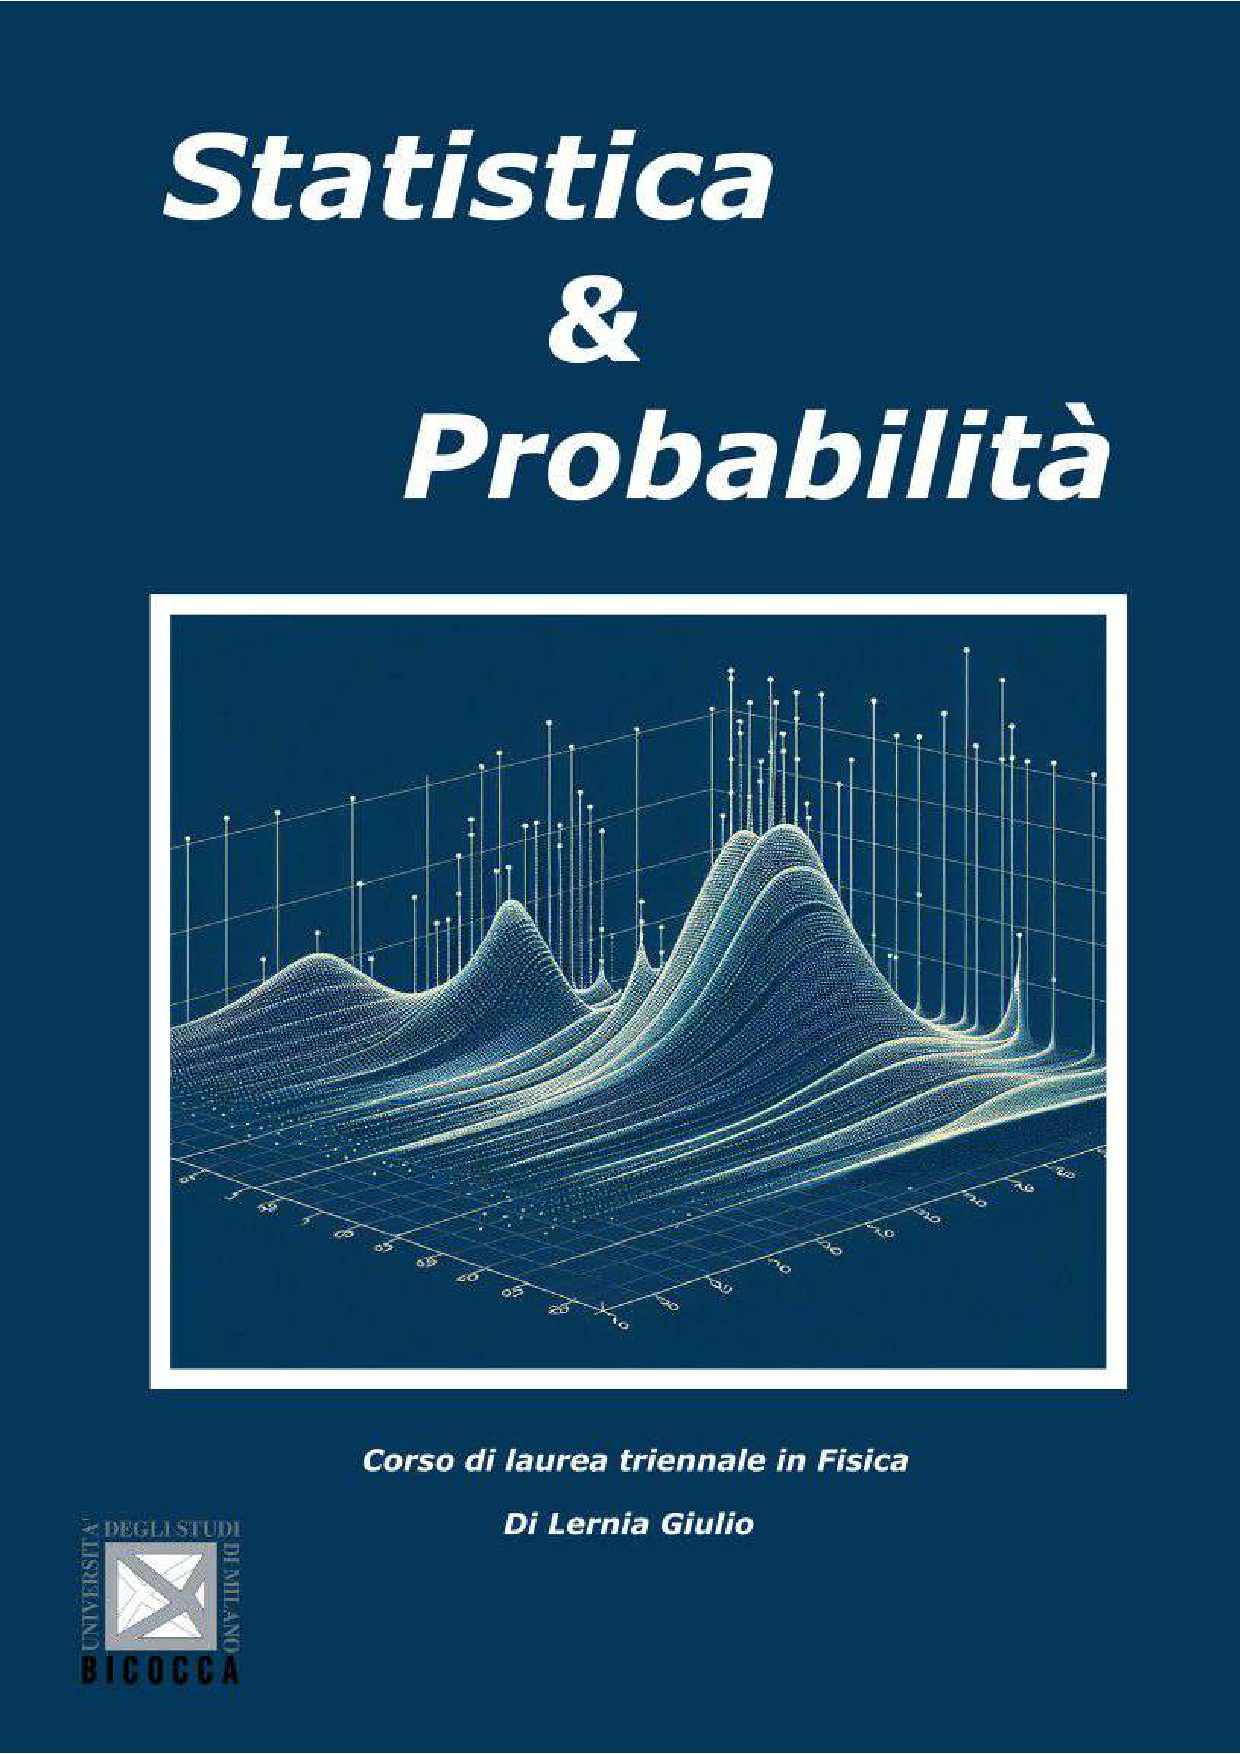
\includepdf[pages = 1,fitpaper]{copertina.pdf}
\tableofcontents


\setcounter{chapter}{0}
\chapter{La probabilit\`{a} e la distribuzione di probabilit\`{a}} 

\section{Assiomi di Kolgomorov}
\textcolor{blue}{Come si definisce la probabilit\'{a} secondo Kolgomorov?}\newline

Consideriamo degli eventi $E_1,E_2 \subset \Omega$ spazio campione, vogliamo costruire definiamo probabilit\'{a} una un funzione $P: \Omega \rightarrow [0,1] $ che soddisfa le seguenti propriet\'{a}:

\begin{itemize}
	\item $P(\Omega) = 1$
	\item $\forall A \subset \Omega$ si ha che $P(A) \geq 0$
	\item $\forall A,B \subset \Omega$,  si ha che $P(A \cup B) = P(A) + P(B) - P(A \cap B)$. Se gli eventi sono indipendenti $ A \cap B = \varnothing $, si ha che $P(A \cup B) = P(A) + P(B)$. 
\end{itemize}

 
\subsection{Definizione di probabilit\'{a} frequentista}

\textcolor{blue}{Come si definisce operativamente la probabilit\'{a} secondo la formulazione frequentista?}\newline

La probabilit\'{a} di un evento A \'{e} definita come il rapporto tra il numero di casi favorevoli (in cui avviene l'evento A) e il numero di casi possibili ( la popolazione). Consideriamo di avere \textbf{N} eventi, e di contare il numero di volte in cui l'evento A, indicandolo come \textbf{n(A)}. Definiamo la probabilit\'{a} di un evento come:
\begin{equation}
	\lim_{N \rightarrow \infty } \dfrac{n(A)}{N}
\end{equation} 

\noindent dove il limite \'{e} inteso in senso probabilistico ovvero al crescere del numero degli eventi.
\subsubsection{Probabilit\'{a} condizionata}

\textcolor{blue}{Che cos'\'{e} la probabilit\'{a} condizionata ?} \newline

Consideriamo una coppia di eventi $A,B \subset \Omega$ definiamo \textbf{probabilit\'{a} condizionata} la probabilit\'{a} che si verifichi l'evento A al verificarsi previamente dell'evento B. 

\begin{equation}
	P(A \vert B) = \dfrac{P(A\cap B)}{P(B)}
\end{equation}

\noindent si dimostra che la probabilit\'{a} condizionata soddisfa gli assiomi di Kolgomorov.

\noindent Nel caso di due eventi indipendenti, ovvero che il verificarsi di B non influenza la probabilit\'{a} che si verifichi A

\begin{equation*}
	P(A \vert B) = P(A \vert \Omega) = P(A)
\end{equation*}

\noindent per due eventi indipendenti possiamo riscrivere la probabilit\'{a} condizionata come:

\begin{equation}
	P(A \cap B) = P(A) \cdot P(B)
\end{equation}

\subsection{Teorema di Bayes}

\textcolor{blue}{Che cosa afferma il teorema di Bayes ?} \newline

Consideriamo due eventi $A,B \subset \Omega$ la probabilit\'{a} nel caso di due eventi non indipendenti possiamo riscrivere la probabilit\'{a} condizionata come:
\begin{equation*}
	P(A \vert B) \cdot P(B) = P(A\cap B) = P(B\vert A) \cdot P(A)
\end{equation*}

dunque l'equazione (1.2) pu\'{o} essere riscritta come : 

\begin{equation}
	P(A \vert B) = \dfrac{P(B \vert A) \cdot P(A)}{P(B)}
\end{equation}

tale espressione definisce il \textbf{teorema di Bayes}. La probabilit\'{a} 
$P(A \vert B)$ viene detta " a posteriori " poich\'{e} permette di calcolare la probabilit\'{a} di 𝐴,sapendo che si \'{e} verificato (o si verificher\'{a} con certezza assoluta) B. \newline
La probabilit\'{a} P(A) si dice invece "a priori" poich\'{e} non è condizionata da alcun altro evento o da alcuna conoscenza che potremmo avere sul suo verificarsi. 

\section{Variabili aleatorie}

\textcolor{blue}{Che cos'\'{e} una variabile aleatoria ?}\newline

Una \textbf{variabile aleatoria} \'{e} una funzione  definita sullo spazio campione a cui viene associato un sottoinsieme misurabile.

\begin{equation}
	X :  \Omega \rightarrow E
\end{equation}
 
 \noindent dove $\Omega$ \'{e} lo spazio di tutti gli esiti possibili, mentre E \'{e} l'insieme degli esiti al verificarsi di un determinato evento.\newline
 
 Nel caso in cui $\Omega \subseteq \mathbb{N}$ si ha che x viene definita \textbf{variabile casuale discreta}. \newline
 Se $\Omega \subseteq \mathbb{R}$, x viene definita \textbf{variabile aleatoria continua}, in questo caso la probabilit\'{a} viene misurata su intervalli $P(a<x<b)$ e non pi\'{u} sui singoli eventi come nel caso di quella discreta. \newline
 
 \noindent \textbf{Esempio:} 
 \begin{itemize}
 	\item Il conteggio del numero di volte in cui compare un certo valore di una misura \'{e} una variabile aleatoria discreta.
 	\item La temperatura \'{e} una variabile aleatoria continua. 
 \end{itemize}
 
 \section{Probability Distribution Function (P.d.f)}
 
 \textcolor{blue}{Che cosa \'{e} una pdf e quali sono le sue propriet\'{a} ?} \newline
 
 Si definisce densit\'{a} di probabilit\'{a} (p.d.f) una funzione che soddisfa le seguenti propriet\'{a}:
 
 \begin{enumerate}
 
 	\item $pdf(x): \Omega \subseteq \mathbb{R} \rightarrow \mathbb{R^+}$
 	\item $P(x < \hat{x} < x +dx) = pdf(x) \cdot dx$
 	\item $P(a < x < b) = \int_{a}^{b}{pdf(x) \cdot dx} \leq 1$
 	\item P(x) = 0, la probabilit\'{a} in una singola misura \'{e} nulla.
 		
 \end{enumerate}
 
 \noindent per la definizione di porbabilit\'{a} nei punti 2) e 3) valgono gli assiomi di Kolgomorov.
 
 
\begin{figure}[!ht]
	\vspace{0.2in}
    \centering
    \subfloat[\centering pdf(x)]{{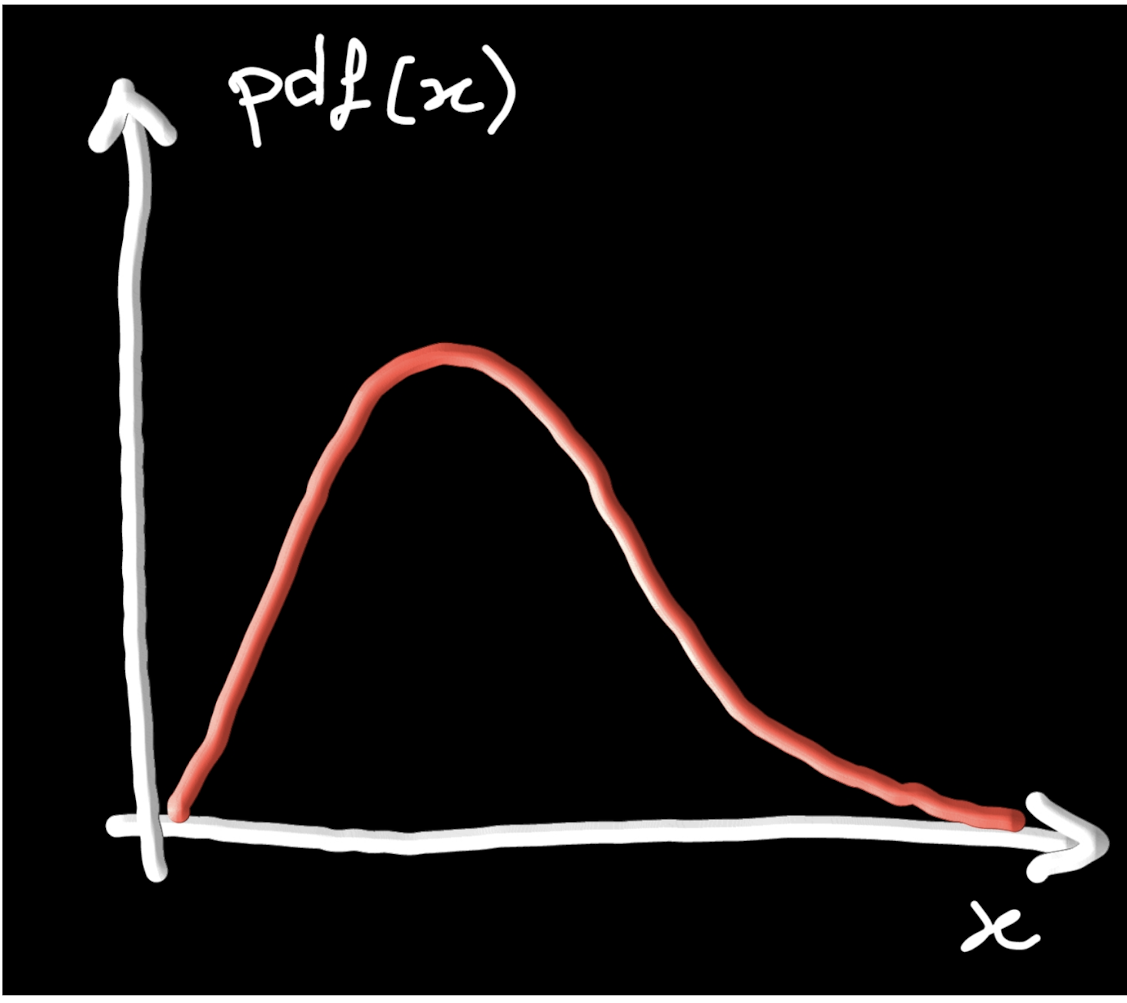
\includegraphics[width=5cm]{pdf} }}
    \qquad
    \subfloat[\centering $P(a<x<b)$]{{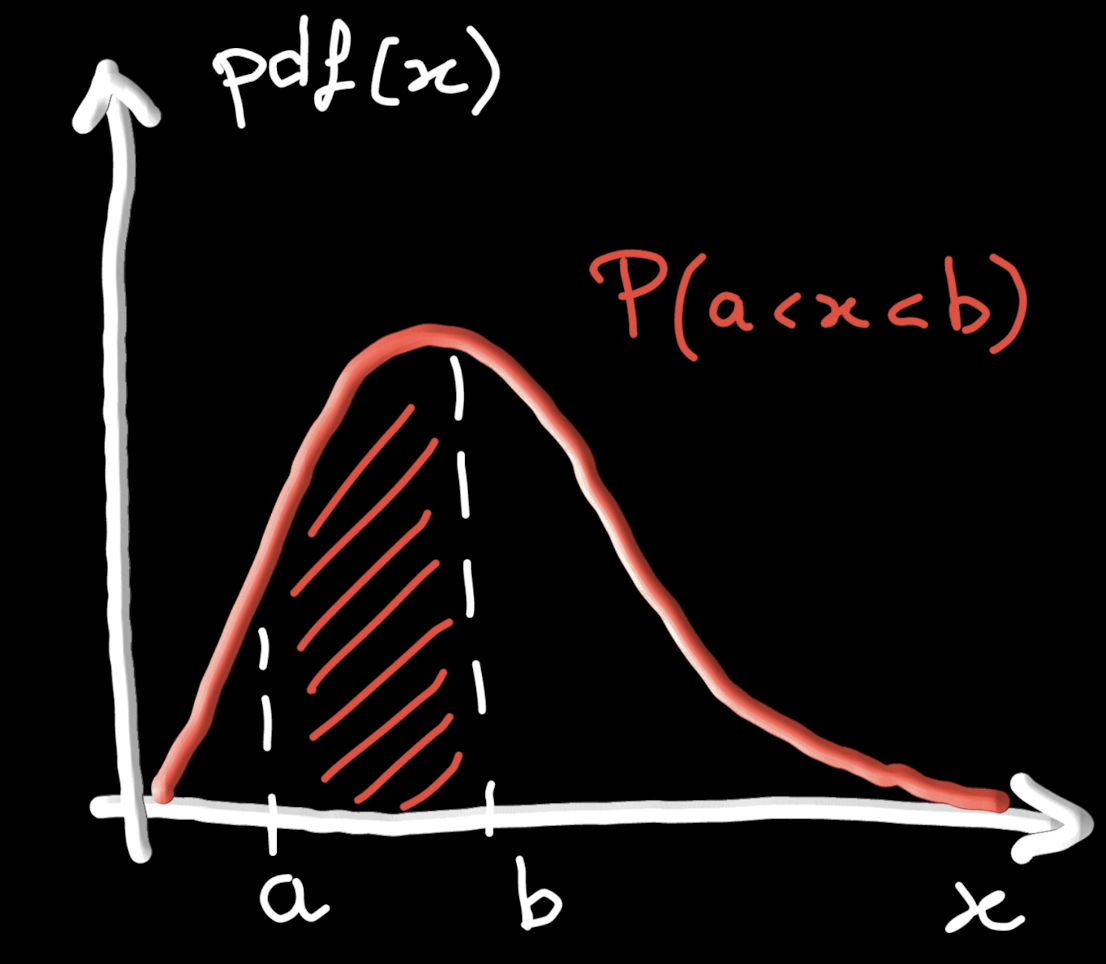
\includegraphics[width=5cm]{prob_pdf} }}
\end{figure}

\subsection{Cumulative distribution function (C.d.f)}

\textcolor{blue}{Che cos\'{e} una c.d.f.?} \newline

Si definisce distribuzione cumulativa la primitiva dell'integrale della pdf di una variabile aleatoria continua \textbf{x}:

\begin{equation}
	cdf(x) = \int_{a}^{x}{pdf(x)dx}
\end{equation}

\noindent ovvero si ha che:

\begin{equation}
	\dfrac{d}{dx}cdf(x)  = pdf(x)
\end{equation}

di conseguenza la cdf(x) descrive l'evolversi della probabilit\'{a} di una variabile casuale.
\subsubsection{Propriet\`{a} di unc cdf}
Una cdf gode delle seguenti propriet\`{a}:
\begin{itemize}
	\item \`{E} una funzione monotona crescente  e definita poisitiva 
	\item cdf(x) $\in [0,1]$
	\item $P(a \leq x \leq b) = cdf(a) - cdf(b)$ 
\end{itemize}
\subsubsection{Corollario}

Esiste una forma analitica della cdf(x) di una r.v. $\iff$ la pdf ammette primitiva. 

\begin{figure}[!ht]
	\vspace{0.2in}
    \centering
    \subfloat[\centering $\int{pdf(x)}$]{{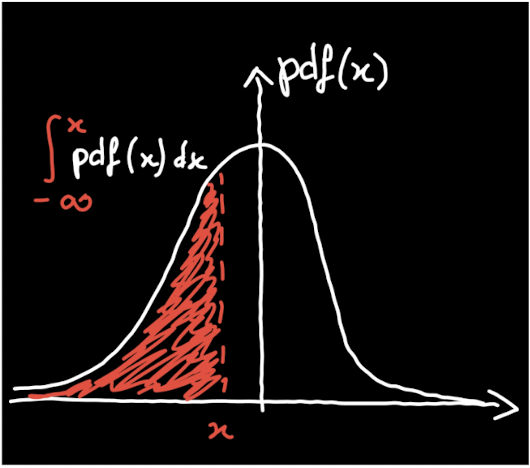
\includegraphics[width=5cm]{int_pdf} }}
    \qquad
    \subfloat[\centering cdf(x)]{{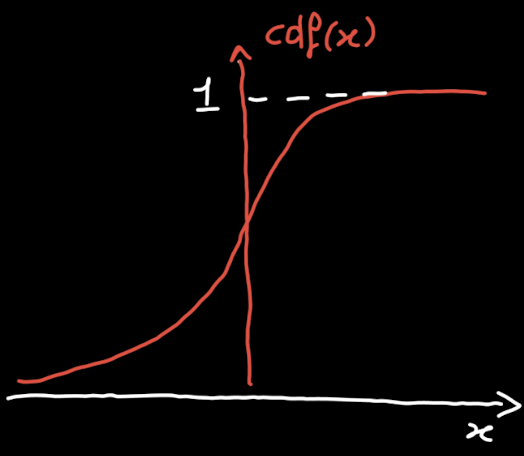
\includegraphics[width=5cm]{cdf} }}
\end{figure}
\newpage
\subsection{Istogrammi}

\textcolor{blue}{Che cos'\'{e} un istogramma ?}\newline


\begin{wrapfigure}{r}{0.\textwidth}
\centering

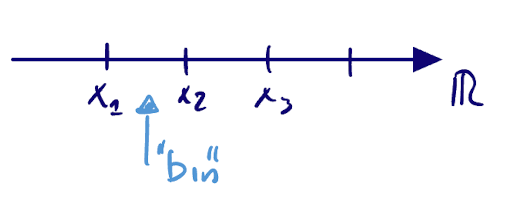
\includegraphics[scale = 0.6]{bin}	

\end{wrapfigure}

Consideriamo una variabile aleatoria x, di cui conosciamo $\{x_i\}_i^N$ valori distinti, utilizziamo tali grandezze come estremi per definire degli intervalli $\omega_{k} = [x_i, x_{i+1}) $ disgiunti tra loro $\omega_{k} \cap \omega_{m} = \varnothing$ per $k \neq m$, sull'asse reale. Tali intervalli vengono definiti \textbf{bin}.

\begin{wrapfigure}[6]{l}{0.\textwidth}

\centering

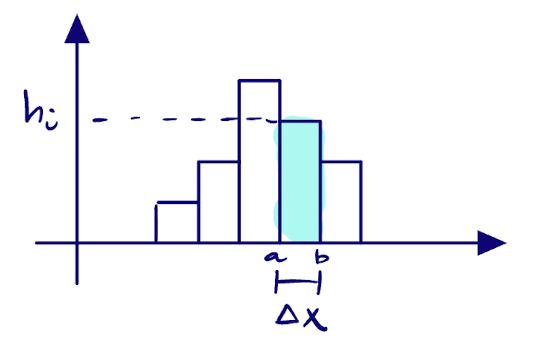
\includegraphics[scale = 0.6]{histogram}	

\end{wrapfigure}

Ripetendo le misure contiamo il numero di volte $n_l$ che un valore compare e cade all'interno di un'intervallo $\omega_k$. 

In questo modo posizionando sull'asse delle ordinate il numero di conteggi $n_l(x)$ si costruisce un istogramma. \newline

\textcolor{blue}{Come si pu\'{o} utilizzare un istogramma per rappresentare una pdf ?}\newline


\begin{wrapfigure}{r}{0.\textwidth}

\centering

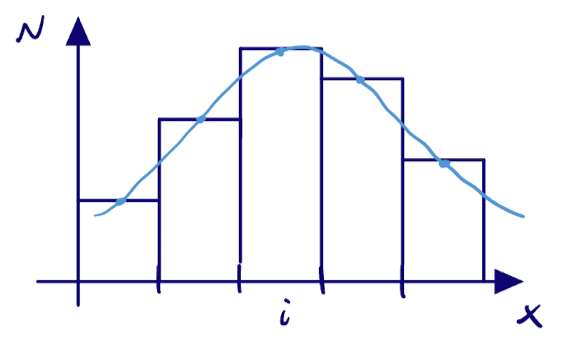
\includegraphics[scale = 0.6]{histo_to_pdf}	

\end{wrapfigure}

All'aumentare del numero di elementi $N \rightarrow \infty$ e diminuendo l'ampiezza dei bin $\Delta x \rightarrow 0 $, ci si riconduce alla nozione di probabilit\'{a} (1.1), in questo modo si passa a una pdf(x) continua.
Per ogni bin \`{e} presente un punto $x_i$ tale che 

\begin{equation*}
	\int_{x_{min}^i}^{x_{max}^i}f(x) dx = f(x_i)\Delta x_i
\end{equation*}
si ha che 
\begin{equation*}
	\lim_{N \rightarrow \infty \atop \Delta \rightarrow 0} \int_{x_{min}^i}^{x_{max}^i}f(x) dx \rightarrow p_i \Rightarrow f(x_i) =  \dfrac{p_i}{\Delta x_i}
\end{equation*}

\subsection{Propriet\`{a} di una probability distribution function}
\textcolor{blue}{Che cosa sono i momenti di una pdf?}\newline

Conoscere l'espressione analitica di una pdf \`{e} spesso poco significativo (soprattuto se la sua espressione non lascia intuire la forma della curva) in altri casi \`{e} impossibile definirla. Di conseguenza per studiare il comportamento di una pdf facciamo affidamento ad alcune grandezze che ne descrivono il comportamento, queste prendono il nome di \textbf{momenti}.

Tali momenti possiamo classificarli come:

\begin{itemize}
	\item $E[x^m] = \int{x^m\cdot pdf(x)dx}$ prendono il nome di \textbf{momenti centrali di ordine m}.
	\item $E[(x-\mu)^m] = \int{(x-\mu)^m \cdot pdf(x)dx}$ prendono il nome di \textbf{momenti centrali}
\end{itemize}

il momento centrale di ordine 1 vale $E[(x-\mu)] = 0$.
\subsection{Valore di aspettazione di una probability distribution function}

\textcolor{blue}{Che cosa \`{e} il valore di aspettazione di una quantit\`{a} rispetto ad una pdf ?}

Data $x \in  \Omega $ variabile aleatoria e $u(x): \mathbb{R} \rightarrow \mathbb{R}$, il valore di aspettazione di u(x) \`{e} definito come:

\begin{equation}
	E[u(x)] = \int{u(x)\cdot pdf(x)dx}
\end{equation}

dove  E[ ] \`{e} un operatore lineare:

\begin{itemize}
	\item $E[x+y] = E[x] + E[y]$
	\item $E[\alpha x] = \alpha E[x] \;\; \forall \alpha \in \mathbb{R}$
\end{itemize}
 Per una variabile aleatoria discreta il valore di aspettazione \`{e} dato da:
 \begin{equation}
 	E[x] = \sum_{i=1}^{+\infty} p_i x_i
 \end{equation}

\subsection{Momenti principali di una pdf per la popolazione e per un campione}

\textcolor{blue}{Che cosa sono e che cosa rappresentano la media, la varianza, l'assimetria e la curtosi di un campione ? e di una popolazione?} \newline

Sia $x \in \Omega $ una variabile aleatoria continua definiamo valore di aspettazione \textbf{media della popolazione} la grandezza:

\begin{equation}
	\mu \equiv E[x] = \int{x \cdot pdf(x)dx}
\end{equation}


\noindent Essa rappresenta il centro della distribuzione di probabilit\`{a} .\newline 
Per un campione di N  misure \textbf{la media} viene definita come: 
\begin{equation}
	\overline{x} = \dfrac{1}{N}\sum_{i=1}^Nx_{i}
\end{equation}
Si definisce \textbf{varianza della popolazione}:
\begin{equation}
	\sigma^2 \equiv V[x] = E[(x-\mu)^2] = \int{(x-\mu)^2 \cdot pdf(x)dx} 	
\end{equation}

la sua radice prende il nome di \textbf{deviazione standard}e definisce l'ampiezza della pdf. La varianza pu\`{o} essere riscritta come:

\begin{equation}
	V[x] = E[x^2] + E[x]^2 = E[x^2] + \mu^2
\end{equation}

Per un campione di N misure \textbf{la varianza} \`{e} data da:

\begin{equation}
	\sigma^2 = \dfrac{1}{N}\sum_{i=1}^N(x- \mu)^2
\end{equation}

mentre \textbf{la deviazione standard} \'{e} di un campione \'{e} data da:

\begin{equation}
	\sigma = \sqrt{\dfrac{1}{N}\sum_{i=1}^N(x- \mu)^2}
\end{equation}

Tra i momenti centrali sono anche presenti la \textbf{skewness} per un campione di N misure:

\begin{equation}
	\gamma_{1} = \dfrac{1}{N}\sum_{i=1}^N \dfrac{(x-\mu)^3}{\sigma^3}
\end{equation}
 e per la popolazione:
 
 \begin{equation}
 	\gamma_{1} = \dfrac{E[(x-\mu)^3]}{\sigma^3}
 \end{equation}
 
 tale grandezza definisce la simmetria di una distribuzione di probabilit\'{a} rispetto al valore centrale dato dal valore di aspettazione $\mu$ per una popolazione. Se una distribuzione \'{e} simmetrica $\gamma_{1} = 0 $.
 
  
\begin{figure}[!ht]

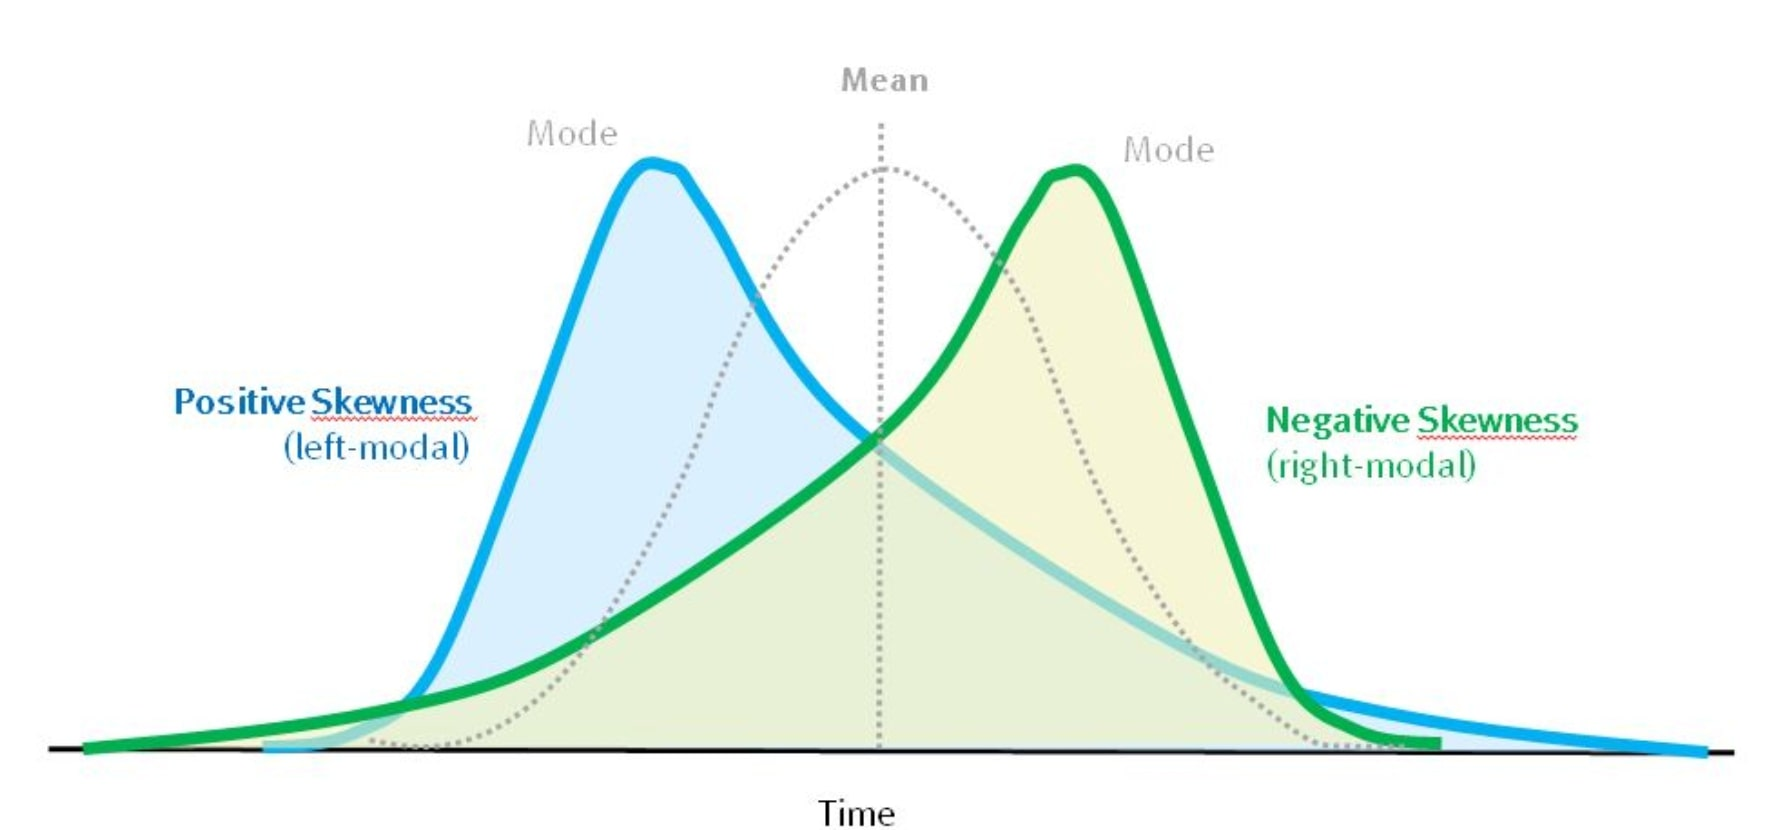
\includegraphics[scale = 0.15]{skew.jpeg}	
\centering
\caption{Simmetria di una distribuzione di probabilit\`{a}}
\end{figure}


Si definisce indice di \textbf{kurtosi} di un campione di N elementi:

\begin{equation}
	\gamma_{2} = \dfrac{1}{N}\sum_{i=1}^N\dfrac{(x-\mu)^4}{\sigma^4}-3
\end{equation}

mentre per la popolazione \`{e} data da:

\begin{equation}
	\gamma_2 = \dfrac{E[(x-\mu)^4]}{\sigma^4} -3
\end{equation}

tale stima fornisce informazioni sul peso delle code della distribuzione, nel senso che per code significative la distribuzione risulter\`{a} pi\`{u} schiacciata nell'intorno del valore $\mu$, mentre per code meno incidenti sar\`{a} pi\'{u} piccata.


\begin{figure}[!ht]

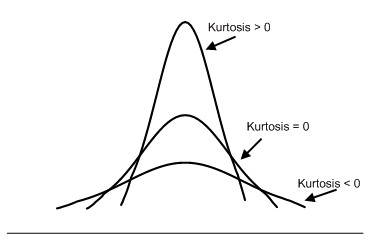
\includegraphics[scale =3.5]{kurtosis.png}	
\centering
\caption{Kurtosi di una distribuzione di probabilit\`{a}}
\end{figure}


\subsubsection{Stime di tendenza centrale}

\textcolor{blue}{Che cosa sono moda, media e mediana di un campione? e di una popolazione ?}


\begin{wrapfigure}[8]{l}{0.\textwidth}

\centering

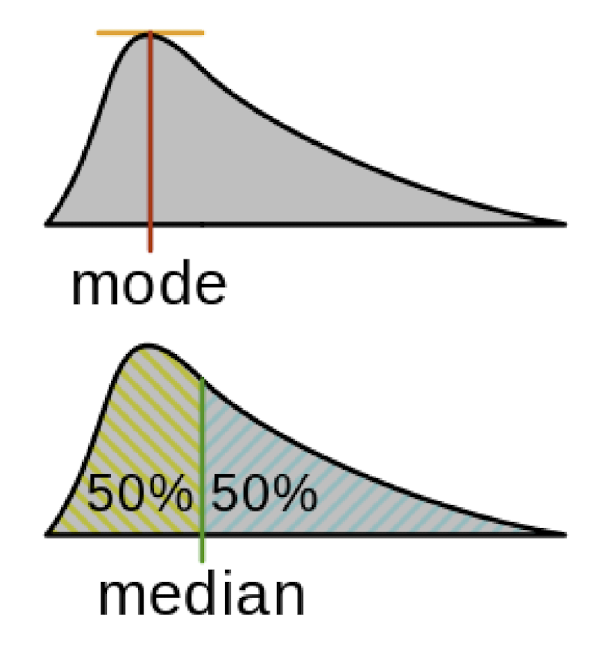
\includegraphics[scale = 0.2]{mod_med}	

\end{wrapfigure}


\noindent Definiamo \textbf{moda} di una popolazione il valore che definisce il massimo della pdf. Mentre per un campione la moda \`{e} definita dalla misura che possiede la frequenza relativa maggiore.\newline

\noindent Mentre si definisce \textbf{mediana} il valore che  divide in due parti uguali la pdf. Nel caso dei campioni le grandezza diventano rispettivamente il valore che compare con maggior frequenza e la misura che divide in due parti eguali il campione.

Per media e mediana di una distribuzione sono unici mentre per una distribuzione pu\`{o} avere pi\`{u} mode, in questi casi si parla di distribuzione \textbf{multimodale}.

 
\begin{figure}[ht]
\vspace{0.3in}
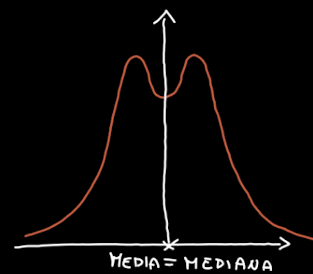
\includegraphics[scale = 0.5]{multimod}	
\centering
\vspace{0.3in}
\caption{Distribuzione multimodale}
\end{figure}

\section{Trasformazioni di distribuzioni di probabilit\`{a}}

Sia x una variabile aleatori continua  che segue una pdf(x) e ipotizziamo di voler costruire una nuova variabile aleatori y legandola ad x mediante una funzione f(x), come definiamo la pdf(y) ?

Sappiamo che la probabilit\`{a} che una misura cada in un intervallo [a,b) \`{e} data da 

\begin{equation*}
	P(a < x< b) = \int_{a}^{b}{pdf(x)dx}
\end{equation*}
\newline

Se effettuiamo un cambio di variabii y=f(x) vogliamo inanzitutto che la trasformazione sia biunivoca dunque f(x) deve essere monotona e continua. In questo modo applicando il teorema per il cambio di coordinate sotto segno d'integrale si ha che:

\begin{equation}
	\dfrac{dy}{dx} = f'(x) \Rightarrow dx = f'(x)^{-1}dy
\end{equation}

di conseguenza:

\begin{equation*}
	P(a < x< b) = \int_{a}^{b}{pdf(x)dx} = \int_{f(a)}^{f(b)}{pdf(y)\vert f'(x)^{-1}\vert dy}
\end{equation*}

per comodit\`{a} si \`{e} posto un modulo affinch\`{e} la funzione sia sempre positiva. In conclusione si ha che:

\begin{equation}
	pdf(y) = pdf(x)\vert f'(x) \vert
\end{equation}
 
 Nel caso in cui abbia pi\`{u} di una dimensione \`{e} necessario che la funzione sia differenziabile e monotona e il modulo della derivata prima della funzione di cambio delle variabili viene sostituita dal modulo del determinante dell'inversa della matrice Jacobiana.
 
 \begin{equation}
 	pdf(\bold{y}) = pdf(\bold{x}) \cdot \vert detJ \vert
 \end{equation}
\newline
\noindent Come si osserva dalle equazioni (1.21) e (1.22) la nuova pdf(y) aumenta o diminuisce di un fattore rispetto alla pdf(x). Comunque sia la probabilit\`{a} in un intervallo resta invariata.

Resta da discutere come cambiano i momenti della distribuzione, per farlo suddividiamo i risultati in due casi:

\subsubsection{Caso in cui il cambio di variabile \`{e} lineare y = ax+b}

Il valore di aspettazione per una pdf(y) dove y = ax+b diventa:

\begin{equation}
	E[y] = \int{y\cdot pdf(y)dy} = \int{(ax+b) \cdot pdf(x)dx = y(\mu_x)}
\end{equation}
 
 analogamente la varianza sar\`{a} data da:
 
 \begin{equation}
 	V[y] = E[y^2] - E[y]^2 = a^2 \cdot V[x]
 \end{equation}

 \subsubsection{Caso in cui il cambio di variabile \'{e} non lineare y = f(x)}
 
 il valore di aspettazione e la varianza di una pdf(y) per y = f(x) non lineare si stima approssimando con il polinomio di Taylor la funzione y(x) in un'intorno di $\mu_x$ al secondo ordine:
 
 \begin{equation*}
 y(x) \approx y(\mu_x) + \dfrac{dy}{dx}\Big\vert_{x = \mu_x}(x-\mu_x) + \dfrac{1}{2}\dfrac{dy^2}{dx^2}\Big\vert_{x = \mu_x}(x-\mu_x)^2
 \end{equation*}
 \newline
 di conseguenza il valore di aspettazione \`{e}:
 
\begin{equation*}
 	E[y] = \int y \cdot pdf(y)dy = y(\mu_x) + \dfrac{dy}{dx}\Big\vert_{x = \mu_x}\int{(x-\mu_x)\cdot pdf(x)dx} + 
 \end{equation*}
 \begin{equation*}
 	+ \dfrac{1}{2}\dfrac{dy^2}{dx^2}\Big\vert_{x = \mu_x} \int{(x-\mu_x)^2 \cdot pdf(x)dx} = 
 \end{equation*}
 
 \begin{equation}
 	= \colorbox{cyan}{\textcolor{white}{$y(\mu_x) + \dfrac{1}{2}\dfrac{dy^2}{dx^2}\Big\vert_{x = \mu_x} \cdot \sigma_{x}^2$}}
 \end{equation}
\newline

Mentre la varianza viene si ottiene dalla relazione:

\begin{equation}
	V[y] = E[y^2] - E[y]^2 = \colorbox{cyan}{\textcolor{white}{$\Big(\dfrac{dy}{dx}\Big \vert_{x = \mu_x}\Big)^2 \cdot \sigma_{x}^2$}} 
\end{equation}
\newline
L'espressione (1.26) \`{e} alla base della formula di propagazione degli errori.

\section{Assenza di memoria per una distribuzione di probabilit\`{a}}

Gli eventi Poissoniani sono indipendenti l'uno dall'altro e la loro probabilit\`{a} di decadimento \`{e} costante, dunque definita q(t) la probabilit\`{a} che non si verifichi un evento in un intervallo di tempo [0,t] si ha che: 
\begin{equation}
	q(t + \delta t) = q(t)q(\Delta t)	
\end{equation}

 la (1.27) definisce l'assenza di memoria di una distribuzione. Si pu\`{o} dimostrare che una distribuzione ha assenza di memoria $\iff$ \`{e} esponenziale.
\vspace{0.05cm}
\par\noindent\rule{\textwidth}{2pt}

\section{Capitolo 1 - Guida allo studio}

\begin{enumerate}
	\item Come si definisce il concetto di probabilità secondo Kolmogorov?
	\item Che legame c`{e} fra gli assiomi di Kolmogorov e i diagrammi di Eulero?
	\item Che cosa \`{e} la probabilità condizionata?
	\item Che cosa afferma il teorema di Bayes?
	\item Come si definisce operativamente la probabilit\`{a}, secondo la formulazione frequentista? 
	\item Che cosa \`{e} una variabile casuale?
	\item Che differenza c'è fra una variabile casuale discreta ed una continua?
	\item Che cosa \`{e} una distribuzione di densit\`{a} di probabilit\`{a} e di quali propriet\`{a} deve godere?
	\item Che cosa \'{e} la distribuzione cumulativa?
	\item Che cosa \'{e} un istogramma?
	\item Come si pu\`{o} utilizzare un istogramma per rappresentare una distribuzione di densit\`{a} di probabilit\`{a}?
	\item Come si effettua un cambio di variabili per una distribuzione di probabilit\`{a}?
	\item Che cosa vuol dire che una distribuzione di probabilit\`{a} ha assenza di memoria ?
	\item Che cosa sono i momenti di una distribuzione di densit\`{a} di probabilit\`{a}?
	\item Che cosa sono i momenti centrali di una distribuzione di densit\`{a} di probabilit\`{a}?
	\item Che cosa è il valore di aspettazione di una quantit\`{a} rispetto ad una distribuzione di densit\`{a} di probabilit\`{a}?
	\item Che cosa sono e che cosa rappresentano la media, la varianza, l'asimmetria e la curtosi di un campione? e di una popolazione?
	\item Che cosa sono moda e mediana di un campione? e di una popolazione?


\end{enumerate}



\setcounter{chapter}{1}
\chapter{Modelli di probabilit\`{a}}
	
\section{La distribuzione Uniforme}

La distribuzione di probabilit\`{a} uniforme per una variabile aleatoria x continua \`{e} definita come:
\vspace{0.3in}

  \begin{minipage}{.5\textwidth}
    \[ pdf(x) = 
	\begin{cases} 
      \dfrac{1}{b-a} & a \leq x \leq b \\
      0 & altrimenti \\ 
   \end{cases}
\]
  \end{minipage}
  \begin{minipage}{.4\textwidth}
    \centering
    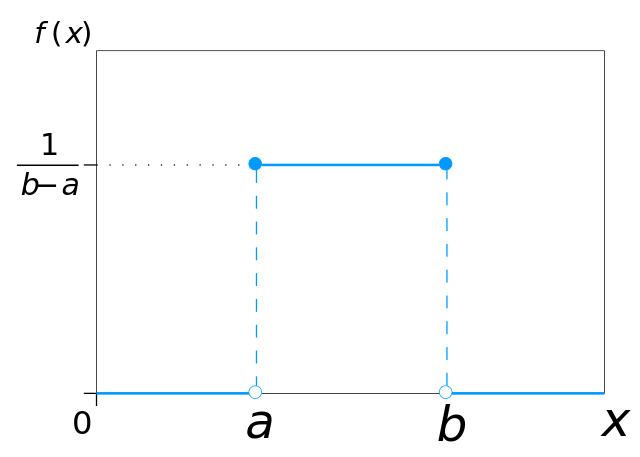
\includegraphics[scale = 0.25]{uniform.png}
 	
  \end{minipage}
\vspace{0.3in}

Tale distribuzione definisce una distribuzione di probabili\`{a} uguale per tutti le variabili aleatorie $x \in \Omega$. 

\subsection{Propriet\`{a} della pdf}
Il valore atteso della distribuzione uniforme e la sua varianza sono date da:

\begin{equation}
	E[x] = \int_{\alpha}^{\beta}{\dfrac{x}{b-a}dx} =\dfrac{b+a}{2} 
\end{equation}

\begin{equation}
	V[x] = \int_{\alpha}^{\beta}{\dfrac{1}{b-a}( x- \dfrac{b+a}{2})^2dx} = \dfrac{(b-a)^2}{12}
\end{equation}
\newline

\noindent Per una distribuzione di questo tipo si ha che la simmetria e la kurtosi rispettivamente hanno valore nullo.\newline
Inoltre tale pdf gode della propriet\`{a} di \textbf{riproduttivit\`{a}} ovvero date due variabili casuali x e y che seguono la pdf uniforme si ha che la nuova variabile aleatoria z = x + y segue una distribuzione di probabilit\`{a} pdf(z) con media $\mu_z = \mu_z + \mu_y$ e varianza $\sigma^2_z = \sigma_x^2 + \sigma_y^2$.\newline

Un'altra propriet\`{a} importante della pdf \`{e} data dal fatto che se si ha una variabile aleatoria x che segue una distribuzione uniforme, la variabile casuale y = f(x) seguir\`{a} anch'essa la medesima distribuzione di probabilit\`{a}.\newline

\noindent Poich\`{e} la pdf possiede una forma analitica \`{e} possibile definirne la cdf:



\vspace{0.3in}

  \begin{minipage}{0.5\textwidth}
  	\begin{equation*}
	cdf(x) = \int_{a}^{x}\dfrac{dx}{b-a} = \dfrac{1}{b-a}(x-a)
\end{equation*}
  \end{minipage}
  \begin{minipage}{.4\textwidth}
    \centering
    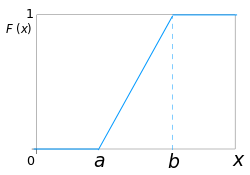
\includegraphics[scale = 0.67]{cdf_uniform.png}

  \end{minipage}
\vspace{0.3in}

\section{La distribuzione Gaussiana (o Normale)}

Data una variabile aleatoria $x \in \Omega $ continua la distribuzione di probabilit\`{a} Gaussiana \`{e} definita come:

\vspace{0.3in}

  \begin{minipage}{0.5\textwidth}
\begin{equation}
	G(x,\mu,\sigma) = \dfrac{1}{\sqrt{2\pi}\sigma} e^{-\dfrac{(x-\mu)^2}{2\sigma^2}}
\end{equation}
  \end{minipage}
  \begin{minipage}{.4\textwidth}
    \centering
    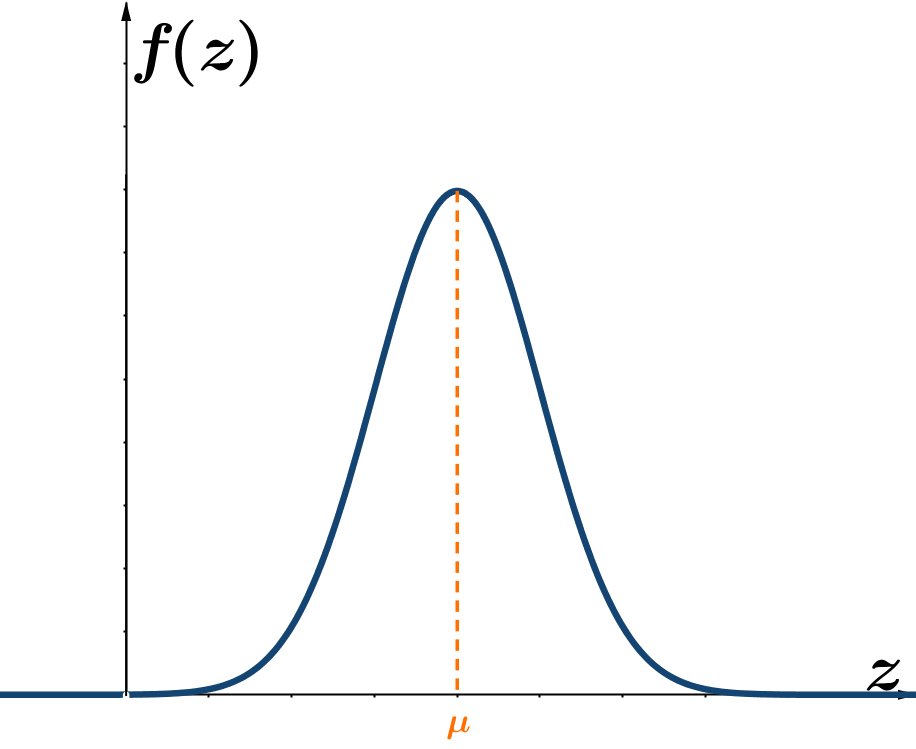
\includegraphics[scale = 0.3]{gaussian.png}

  \end{minipage}
\vspace{0.3in}

Per una distribuzione Gaussiana si ha che la media, la moda e la mediana coincidono essendo una distribuzione simmetrica ovvero $\gamma_{1},\gamma_2 = 0$. Media, Varianza e deviazione standard coincidono con quelle definite al capitolo precedente. Gode della propriet\`{a} di \textbf{riproduttivit\'{a}} definita nella sezione della distribuzione uniforme.\newline

\noindent Una caso speciale di Gaussiana \`{e} quella \textbf{standardizzata} che \`{e} espressa come:

\begin{equation*}
	G(x) = \dfrac{1}{\sqrt{2\pi}}\; e^{-\dfrac{x^2}{2}}
\end{equation*}

\subsection{Distribuzione cumulativa di una Gaussiana}

La pdf Gaussiana non ammette primitiva e la sua cdf viene calcolata numericamente e prende il nome di \textbf{funzione d'errore}, abbreviata con erf(x).

\vspace{0.3in}

  \begin{minipage}{0.5\textwidth}
\begin{equation*}
	erf(x) = \dfrac{1}{\sqrt{2\pi}} \int_{-\infty}^{a}{e^{-\dfrac{x^2}{2}}}
\end{equation*}
  \end{minipage}
  \begin{minipage}{.4\textwidth}
    \centering
    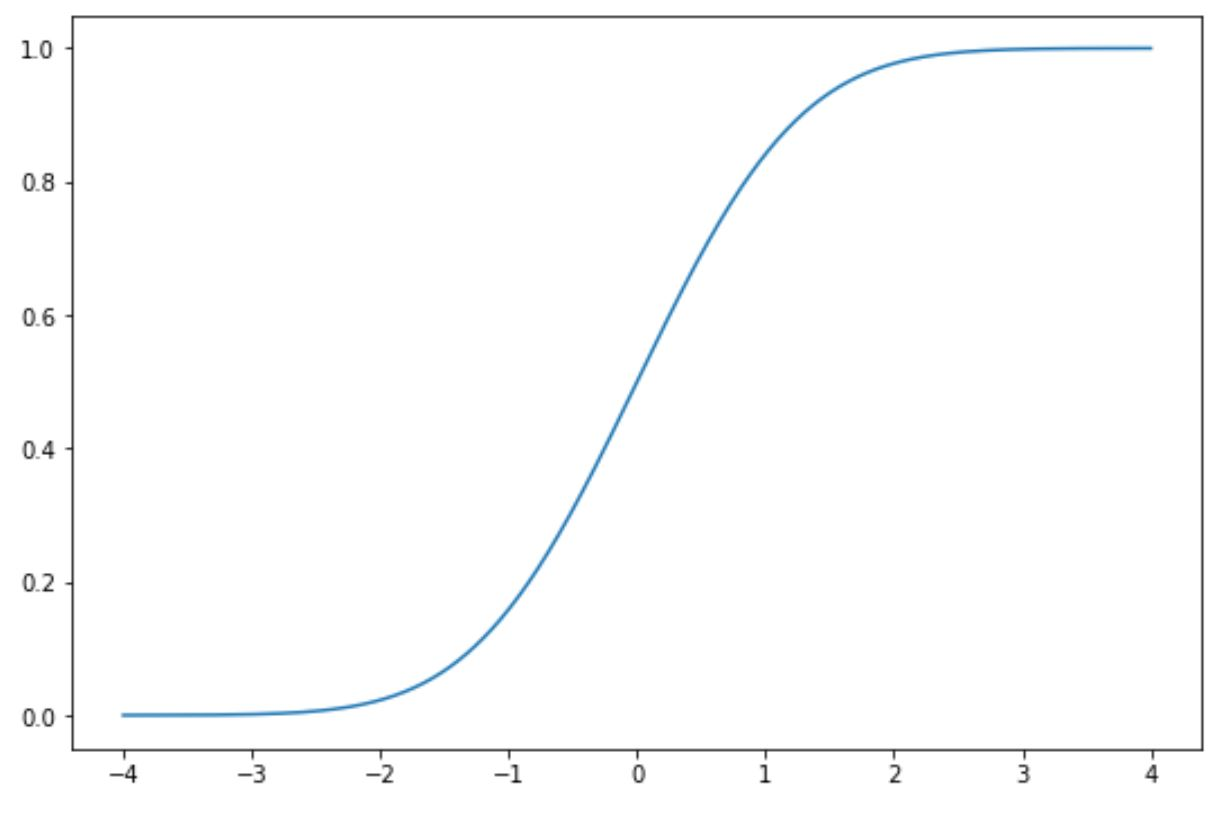
\includegraphics[scale = 0.42]{gauss_cdf.jpeg}

  \end{minipage}
\vspace{0.3in}

\subsection{Teorema Centrale del Limite} 

La distribuzione Gaussiana \`{e} particolarmente importante poich\`{e} per essa vale un importante risultato. 

\subsubsection{Teorema}

Si ipotizzi di avere N variabile aleatorie $\{x_i\}_i^N$ indipendenti tra loro e ciascuna di esse segue una distribuzione di probabilit\`{a} $f_i(x)$ con $E[x_i] < \infty$ e $V[x_i] < \infty$, e definiamo una nuova variabile aleatoria $s = \sum_{i=1}^Nx_{i}$ che segue una distribuzione pdf(s), allora si avr\`{a} che al crescere del numero di variabili:
\begin{equation*}
	\lim_{N \rightarrow \infty} pdf(s) \rightarrow G(s,\mu_s,\sigma_s)
\end{equation*}

dove $\mu_s =\sum_{i=1}^N \mu_i$ e $\sigma_s^2 = \sum_{i=1}^N \sigma^2_i$ .

\subsubsection{Corollario della media}

Date N variabili aleatorie $\{x_{i}\}_{i}^N$ indipendenti ed identicamente distribuite, ovvero che per ogni variabile si ha la stessa distribuzione di probabilit\`{a} f(x) e ipotizzando che $\forall i$ si ha che $\mu_i$ e $\sigma_i^2$ siano finite , definita una nuova variabile aleatoria $\overline{x} = \dfrac{\sum_{i=1}^N x_{i}}{N}$ che segue una pdf $f(\overline{x})$, si ha che al crescere del numero di variabili:

\begin{equation*}
	\lim_{N \rightarrow \infty} f(\overline{x}) \rightarrow G(\overline{x},\mu,\frac{\sigma}{\sqrt{N}})
\end{equation*}

dunque si ha che la pdf delle medie campionarie di un campione che cresce converge alla distribuzione Gaussiana.


\subsection{Conseguenze del TCL}

 Quando effettuiamo una misura in un esperimento in generale possiamo definirla come la somma del valore vero $x_0$ e di un errore $\epsilon$ che \`{e} una variabile aleatoria. 
 
 \begin{equation*}
 	x = x_0 + \epsilon
 \end{equation*}
La maggior parte delle misure che si effettuano sono la somma di variabili aleatorie, come per esempio errori intriseci ed errori sperimentali. Per esempio quando misuriamo un oggetto con un metro, inseriamo all'interno della misura degli errori, che possono dipendere sia dalle condizioni sperimentali che dall'operatore (Diottrie, stabilit\'{a} del polso, ecc...), tali errori si sommano tra loro. Il teorema centrale del limite risulta essere importante perch\'{e} ci dice che la somma di tali errori al crescere della dimensione del campione segue una distribuzione di probabilit\'{a} Gaussiana, permettendoci di applicare alcuni metodi statistici per la stima dei parametri e garantendo delle propriet\'{a} significative alla stima.

\section{Distribuzione di probabilit\`{a} Log-normale}

Presa una variabile aleatoria $x \in \Omega $ che segue una distribuzione Gaussiana, costruiamo una nuova variabile aleatoria y legata alla precedente dalla relazione $y = e^x$, in questo modo si definisce la distribuzione log-normale applicando un cambio di variabile alla G(x) di partenza, il metodo con cui si effettua un cambio di variabile verr\`{a} presentato nei capitoli successivi.

\begin{equation*}
	f(x,\mu,\sigma) = \dfrac{1}{\sqrt{2\pi}\sigma}\;\dfrac{1}{x}\; e^{-\frac{(log(x)-\mu)^2}{2\sigma^2}}
\end{equation*} 

\subsection{Propriet\`{a} della log-normale}

Il valore di aspettazione e varianza della log-normale sono dati da:

\begin{equation}
	E[x] = e^{(\mu + \frac{1}{2}\sigma^2)}
\end{equation}

\begin{equation}
	V[x] = e^{(2\mu + \sigma^2)}e^{(\sigma^2-1)}
\end{equation}

\section{Distribuzione di Probabilit\`{a} di Bernoulli}

Sia $x \in \Omega = \{0,1\}$ una variabile aleatoria discreta, a cui \`{e} possibile associare una probabilit\`{a} $p \in [0,1]$. Definiremo che l'evento x si \`{e} realizzato con successo quando P(x = 1) = p, mentre l'insuccesso con P(x = 0)= (1-p). Dunqua la pdf(x) \`{e} data da:

\begin{equation*}
	f(x,p) = p^x(1-p)^{1-x}
\end{equation*}

\subsection{Propriet\`{a} della distribuzione Bernoulliana}

Per una distribuzione di Bernoulli media e varianza sono date:

\begin{equation}
	E[x] = \sum_{\{0,1\}}xf(x,p) = p
\end{equation}

\begin{equation}
	V[x] = \sum_{\{0,1\}}(x-p)^2f(x,p) = p(1-p)
\end{equation}

\section{Distribuzione di Probabilit\`{a} Binomiale}

Si consideri un insieme di N osservazioni indipendenti, che seguono una distribuzione di Bernoulli. Contiamo il numero di volte k in cui l'evento ha successo rispetto al numero di tentativi effettuati, tale insieme \`{e} il nostro campione. Se si ripete l'esperimento effettuando sempre N tentativi, il numero di successi n sar\`{a} distribuita secondo la distribuzione binomiale:

\begin{equation*}
	B(k \vert N,p) = \binom{N}{k}p^k(1-p)^{N-k}
\end{equation*} 
\newline
notare che a differenza delle distribuzioni viste fino ad ora, la distribuzione binomiale in realt\`{a} rappresenta la probabilit\`{a} stessa di una variabile aleatoria k, come anche la Bernoulliana.

\subsection{Propriet\`{a} della distribuzione binomiale}

Per una distribuzione binomiale il valore di aspettazione e la varianza sono definite da :

\begin{equation}
	E[k] = \sum_{k}^\infty k \binom{N}{k}p^k(1-p)^{N-k} = Np
\end{equation}

\begin{equation}
	V[k] = E[k^2] - E[k]^2 = Np(1-p)
\end{equation}

\noindent la simmetria \`{e} data da:
\begin{equation}
	\gamma_1 = \dfrac{1-2p}{\sqrt{Np(1-p)}}
\end{equation}

dove $\gamma_1 \rightarrow 0 $ per $N \rightarrow \infty $ o per $p = \frac{1}{2}$.\newline

la kurtosi invece si esprime come:
\begin{equation}
	\gamma_2 = \dfrac{1-6p}{Np(1-p)}
\end{equation}

dove $\gamma_2 \rightarrow 0$ per $N \rightarrow \infty$ e $p = \frac{1}{6}$.
Inoltre la distribuzione binomiale gode della propriet\`{a} di \textbf{riproduttivit\`{a}}
\subsection{La densit\`{a} di probabilit\'{a} di un'istogramma}



Consideriamo di avere una variabile aleatoria x di cui effettuiamo N misurazioni, ciascuna misurazione segue una pdf(x). 

\begin{wrapfigure}{l}{0.\textwidth}
\centering

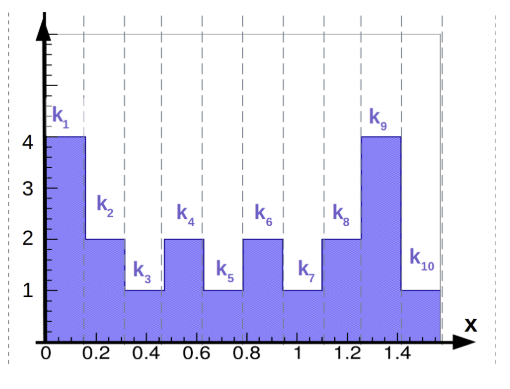
\includegraphics[scale = 0.33]{binning}	

\end{wrapfigure}

\noindent L'operazione \`{e} equivalente a campionare N volte una pdf(x). Posto che le $\{x_{i}\}_{i}^N$ misure siano il campione di riferimento, la statistica si pone obbiettivo quello di ricostruire partendo dal campione le caratteristiche di una pdf(x).
\begin{wrapfigure}{r}{0.\textwidth}
\centering
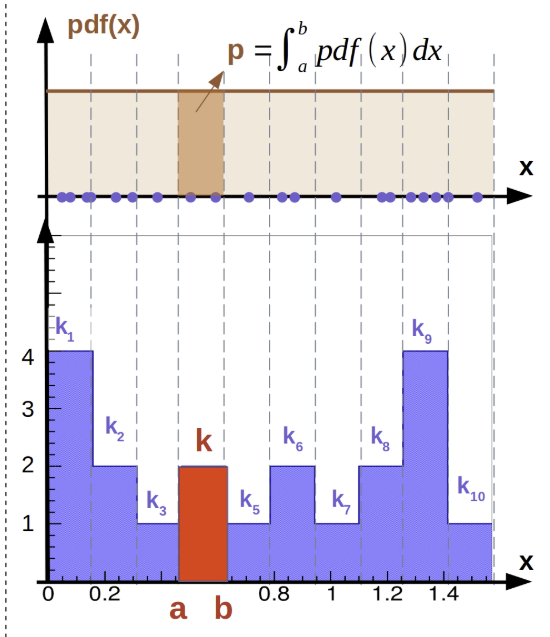
\includegraphics[width = 1.9in]{Bernouli_Histo}	

\end{wrapfigure}
\noindent Per farlo si procede a costruire un istogramma e a contare il numero di eventi $k_{i}$ che cadono all'interno di un bin e rappresentare tale numero con una barra. Il numero di misure $k_i$ che cade all'intero di un bin \`{e} una variabile aleatoria.


Di conseguenza studiando il comportamento di un singolo bin [a,b), il numero di misure $k_{i}$ \`{e} descritto da una distribuzione di probabilit\`{a}, poich\`{e} un fenomeno cade o non cade all'interno dell'intervallo la pdf($k_i$) \`{e} quella di Bernoulli. 

Reiterando l'esperimento sullo stesso bin il numero di successi $k_{i}$ seguir\`{a} una pdf(k) di una binomiale $B(k \vert N,p)$ dove la probabilit\`{a} \`{e} $ p = \int_{a}^{b}{pdf(x)dx}$ sull'intervallo del bin associato.

 Un conteggio di misure \`{e} soggetto a fluttuazioni statistiche, e al crescere del numero delle misure l'istogramma assumer\`{a} la distribuzione di probabilit\`{a} pdf(x) della variabile aleatoria X misurata.
\newline
\noindent Se ipotizziamo che X abbia una distribuzione uniforme, valore di aspettazione e varianza di un conteggio coincideranno con quella della distribuzione Binomiale.

I metodi statisti che possono essere applicati a misure binnate richiedono che i conteggi $k_{i}$ siano variabili aleatorie indipendenti, affinch\`{e} tale condizione risulti essere verificata si hanno due strategie possibili:

\begin{itemize}
\item
\noindent Se la dimensione dei bin \`{e} piccola e la probabilit\`{a} \`{e} sufficientemente piccola allora la covarianza \`{e} pressoch\`{e} nulla. Di conseguenza le variabili $k_i$ sono indipendenti tra loro e dunque ciascuan distribuita come una binomiale.
\item
\noindent Se il numero di eventi N \`{e} molto grande e la probabilit\`{a} $p_i$ \`{e} piccola la distribuzione di probabilit\`{a} dei conteggi \`{e} approssimabile a quella di una distribuzione Poissoniana. 
\section{Distribuzione Multinomiale}

\end{itemize}

Considerando quando discusso nella sezione precedente per ogni singolo bin che si \`{e} costruito nell'istogramma, si definisce una probabilit\`{a} multinomiale:

\begin{equation}
	Multi(k_1,k_2,...,p_1,p_2,...) = \dfrac{N!}{k_1!\cdot k_2! \cdots}p^{k_{1}}p^{k_2}\cdots
\end{equation}
\newline
\noindent Valore di aspettazione e varianza rimangono le medesime per ogni singolo bin, solo che i conteggi $k_i$ non sono variabili aleatorie indipendenti tra loro, in questo caso si ha la \textbf{covarianza}:

\begin{equation}
	cov[k_i,k_j] = -N \cdot p_i \cdot p_j 
\end{equation}

\section{Distribuzione di Poisson}

La distribuzione di Poisson \`{e} una distribuzione di probabilit\`{a} discreta che esprime la probabilit\`{a} che un numero di eventi indipendenti si verifichi in un certo intervallo di spazio o tempo fissato con una frequenza media costante. il verificarsi dell'evento a un tempo t non influenza il verificarsi del medesimo in un intervallo di tempo successivo o precedente  al tempo t.
La probabilit\`{a} di contare k eventi in un intervallo di tempo unitario \`{e}:

\begin{equation}
	Poiss(k,\lambda) = \dfrac{e^{-\lambda} \cdot \lambda^k}{k!}
\end{equation}

lo spazio campione rispetto alla quale \`{e} definita \`{e} tutto $\mathbb{N}$



\subsection{Propriet\`{a} della distribuzione di Poisson}

Il valore di aspettazione e la varianza della distribuzione di Poisson sono:

\begin{equation}
	E[k] = \sum_{k=0}^{\infty}k \cdot \dfrac{e^{-\lambda} \cdot \lambda^k}{k!} = \lambda 
\end{equation}

\begin{equation}
	V[k] = \sum_{k=0}^{\infty} (k - \lambda)^2 \cdot \dfrac{e^{-\lambda} \cdot \lambda^k}{k!} = \lambda 
\end{equation}

si nota che all'aumentare della media aumenta anche la varianza. \newline

L'indice di simmetria e kurtosi sono dati da:

\begin{equation}
	\gamma_1 = \dfrac{1}{\sqrt{\lambda}}
\end{equation}

\begin{equation}
	\gamma_2 = \frac{1}{\lambda}
\end{equation}

per $\lambda \rightarrow \infty $ la distribuzione di Poisson diventa pi\`{u} simmetrica. Inoltre la distribuzione di Poisson gode della propriet\`{a} di \textbf{riproduttivit\`{a}}.


\subsection{Da eventi Poissoniani all'esponenziale}

Il modello su cui si basa la distribuzione di Poisson \`{e} dato dalle seguenti assunzioni:

\begin{itemize}
	\item la probabilit\`{a} che un evento avvenga in un intervallo di tempo [t,t+dt] \`{e} data da $p\cdot dt$, dove p \`{e} un valore costante e indipendente da t;
	\item la probabilit\`{a} di avere pi\`{u} di un evento nell'intervallo dt \`{e} nulla.
	\item gli eventi sono indipendenti tra loro.
\end{itemize}

Definiamo E = \{ nessun evento avvenuto in [0,t+dt]\} e la funzione q(t) = \{probabilit\`{a} di nessun evento in [0,t]\}, posta I come l'informazione a priori (ex: tempo di decadimento medio) si ha che la probabilit\`{a} che si verifichi E essendosi gi\`{a} verificato I \`{e}:

\begin{equation}
	P(E\vert I) \equiv q(t+dt)
\end{equation} 

Dove q ha come argomento la lunghezza degli intervalli di tempo; possiamo riformulare E come l'intersezione di due eventi $E_1 =$ \{0 eventi in [0,t] \} ed $E_2 = $ \{ 0 eventi in [t,t+dt]\}, dunque 2.19 pu\`{o} essere riscritta come:

\begin{equation*}
	P(E \vert I) = P(E_1,E_2 \vert I) = P(E_1 \vert I)P(E_2 \vert E_1 ,I)
\end{equation*}

poich\`{e} per ipotesi $E_{1}$ ed $E_{2}$ sono indipendenti dato che il verificarsi di un evento in un intervallo di tempo non influenza il verificarsi del medesimo evento in un intervallo successivo si ha che:

\begin{equation}
	P(E \vert I) = P(E_1 \vert I)P(E_2 \vert I)
\end{equation}

dove $P(E \vert I) = q(t+dt)$ , $P(E_1 \vert I) = q(t)$ e $P(E_2 \vert I) = 1-pdt$. Dunque:

\begin{equation}
	q(t+dt) = q(t)\cdot (1-pdt) \Rightarrow \dfrac{q(t+dt)-q(t)}{dt} = -q(t)p
\end{equation}

questo \`{e} equivalente all'equazione differenziale al primo ordine:

\begin{equation*}
	\dfrac{dq}{q} = -p \cdot dt \iff q(t) = q(0)e^{-pt}
\end{equation*}

dove q(0) \`{e} determinata normalizzando la distribuzione di probabilit\`{a}. \textcolor{cyan}{Per eventi che occorono in modo Poissoniano la probabilit\`{a} di non avere eventi in un intervallo [0,x] \`{e} data da una esponenziale}.

Per comodit\`{a} poniamo q(0)=1. Definiamo $A = \{ 1 \; evento \; in \; [t_1,t_1+dt_1] \}$ ed B = \{ 0 eventi in [0,$t_1$]\} definiamo:

\begin{equation}
	P(A,B \vert I) = P(A \vert I) \cdot P(B \vert I) = e^{-pt}(p \cdot dt)
\end{equation} 

ipotizzando di costruire una catena di eventi in cui si realizza e non si realizza un evento per tempi ordinati si ha che:
\begin{equation}
	P(A,B \vert I) = e^{-pt_1} \cdot p \cdot dt_1 \cdot e^{-p(t_2-t_1)} \cdot p \cdot dt_2 \cdots = e^{-pt}p^ndt_1 \cdots dt_n
\end{equation}

Per definire una probabilit\`{a} che si realizzino n eventi in un intervallo di tempo [0,t], a prescindere dal tempo preciso in cui avvengono, dobbiamo sommare le probabilit\`{a} definite in (2.23):

\begin{equation}
	P(n \vert p,t,I) = e^{-pt}p^n \int_0^{t_2}dt_{1} \cdot \int_{0}^{t^3}dt_{2} \cdots \int_{0}^{t}dt_n
\end{equation}

il prodotto d'integrali ha come soluzione $\frac{t^n}{n!}$ e dunque:

\begin{equation}
	P(n \vert p,t,I) = \dfrac{(pt)^n}{n!}e^{-pt} = \dfrac{\lambda^n}{n!}e^{-\lambda}
\end{equation} 

\section{Distribuzione Esponenziale}

La distribuzione esponenziale \`{e} la distribuzione dei tempi che intercorrono tra due eventi Poissoniani, ovvero la probabilit\`{a} che nessun evento si verifichi. Infatti consideriamo k il numero di eventi definiti da una pdf Poissoniana con frequenza p, avvenuti in un intervallo di tempo [0,t]. Allora si ha:

\begin{equation*}
	P(k,p) = \dfrac{(pt)^k}{k!}e^{-pt}
\end{equation*}
\newline
 Se misuriamo la probalit\`{a} che nessun evento si verifichi in un tempo $t < T$ si avr\`{a}:

\begin{equation*}
	P(0 \vert p,t) = \dfrac{(pt)^0}{0!}e^{-pt} = e^{-pt}
\end{equation*}
\newline
 e si ha dunque una pdf Poissoniana. Se rileviamo il medesimo evento per $T > t$ si avr\`{a} che la probabilit\`{a} dell'evento avvenuto al tempo T \`{e} descritta dalla medesima pdf per il tempo t antecedente:

\begin{equation*}
	P(0 \vert p, T>t) = P(0 \vert p, t) = e^{-pt}
\end{equation*}
 Dunque la distribuzione di probabilit\`{a} che intercorre da tra due eventi Poissoniani \`{e} esponenziale.
\begin{figure}[ht]
\vspace{0.2in}
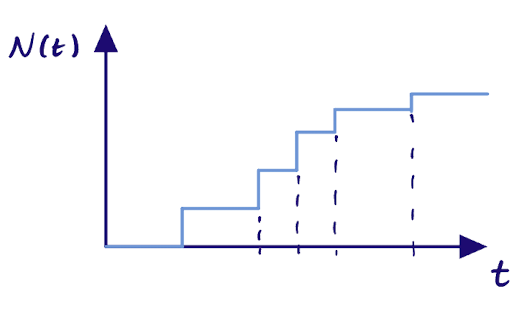
\includegraphics[scale = 0.45]{pois}	
\centering
\vspace{0.2in}
\end{figure}

ed \`{e} definita da:

\begin{equation}
	pdf(t,\lambda) = \lambda \cdot e^{-\lambda t}
\end{equation}

dove $\tau$ = E[t] \`{e} il tempo medio tra due eventi consecutivi, e vale la relazione $\lambda = \frac{1}{\tau}$ dove $\lambda$ \`{e} il parametro della Poissoniana che determina la frequenza media di eventi. 

\subsection{Propriet\'{a} della distribuzione esponenziale}

Il valore di aspettazione e varianza sono date dalle quantit\`{a}:

\begin{equation}
	E[t] = \tau = \dfrac{1}{\lambda}
\end{equation}

\begin{equation}
	V[t] = \tau^2 = \dfrac{1}{\lambda^2}
\end{equation}

mentre i parametri di simmetria della distribuzione dati da simmetria e kurtosi:

\begin{equation}
	\gamma_1 = 2
\end{equation}

\begin{equation}
	\gamma_2 = 6
\end{equation}

come si osserva dai momenti essendo $\gamma_1$ e $\gamma_2$ costanti la distribuzione esponenziale non pu\`{o} tendere ad una Gaussiana al crescere del numero die venti.

\subsection{Decadimento Radioattivo}

Si consideri un campione di materiale radioattivo contenente $N_{0}$ nuclei al tempo t=0 per un singolo nucleo padre la probabilit\`{a} di decadimento segue una distribuzione esponenziale il cui $\tau$ tempo medio di decadimento \`{e} dato dalla meccanica quantistica. Gli eventi di decadimento sono \textbf{indipendenti} tra di loro.
\newline
La variazione del numero dei nuclei in un intervallo di tempo $\Delta t$ sar\`{a} proporzionale al numero di nuclei restanti:

\begin{equation}
	-\dfrac{dN}{dt} = \lambda N
\end{equation}

dove $\lambda$ \`{e} la frequenza media di decadimento. Di conseguenza il decadimento radioattivo \`{e} definito dalla funzione:

\begin{equation}
	N(t) = N_{0}e^{-\lambda t}
\end{equation}

che possiamo riscrivere come :

\begin{equation}
	N(t) = N_{0} e^{-\frac{t}{\tau}}
\end{equation}

Se $\tau >> t$ tempo di osservazione, la frequenza media dei decadimenti \`{e} costante nel tempo e di conseguenza la probabilit\`{a} di osservare k decadimenti in un campione di N nuclei \`{e} data dalla distribuzione di Poisson con $\lambda = \frac{1}{\tau}$.

\section{Comportamenti Asintotici delle distribuzioni}

\subsection{Propriet\`{a} asintotiche della Binomiale e Poissoniana}

\subsubsection{Binom(k$\vert$N,p) $\rightarrow$ Poisson(k,$\mu = N \cdot p$)}
La relazione tra distribuzione Binomiale e Poissoniana si costruisce assumendo di prendere un intervallo $\Delta t$ e di dividerlo in N intervalli di dimensione dt tali per cui:

\begin{itemize}
	\item in ciascun dt cada uno solo evento( tale ipotesi \`{e} verificata solo se il numeri di eventi \`{e} molto grande);
	\item la probabilit\`{a} in un singolo intervallo dt \`{e} $p = \dfrac{\lambda}{N}$ ed \`{e} finita;
	\item gli eventi che cadono in ogni intervallo dt sono indipendenti tra loro.
	
\end{itemize}

Essendo gli eventi indipendenti tra loro per ipotesi ciascuno di essi segue una distribuzione di Bernoulli. Tali condizioni consentono di usare una distribuzione binomiale per descrivere eventi Poissoniani.

Per induzione si ha che per k=0 posto $\lambda = N \cdot p$

\begin{equation*}
	B \Big (0\vert N, \dfrac{\lambda}{N} \Big ) = \Big (1- \dfrac{\lambda}{N} \Big )^N =_{N \rightarrow \infty} \dfrac{\lambda^0}{0!}e^{-\lambda}
\end{equation*}

dunque la relazione per k-1 sar\`{a} verificata e:

\begin{equation*}
	B \Big (k-1\vert N,\frac{\lambda}{N} \Big ) =_{N \rightarrow \infty} \dfrac{\lambda^{k-1}}{(k-1)!} e^{- \lambda}
\end{equation*}

Allora si dimostra che dall'espressione binomiale:

\begin{equation*}
	\dfrac{B \Big (k  \vert N , \dfrac{\lambda}{N}\Big)}{B \Big(k-1 \vert N, \dfrac{\lambda}{N} \Big) } = \dfrac{Np- (k-1)p}{k(1-p)} \approx_{p \rightarrow 0} \dfrac{\lambda}{k}
\end{equation*}


 dunque:
 
 \begin{equation*}
 	B \Big (k  \vert N , \dfrac{\lambda}{N}\Big) = \dfrac{\lambda}{k} \cdot B \Big(k-1 \vert N, \dfrac{\lambda}{N} \Big) \rightarrow \dfrac{\lambda^{k}}{k!} e^{-\lambda}
 \end{equation*}
\newline

Si dimostra inoltre che data una distribuzione Binomiale $B(k \vert N,p) \rightarrow G(k,\mu,\sqrt{\mu})$ al crescere del numero di misure $N \rightarrow \infty $ per $\mu = N \cdot p$ costante.
\newline

Vale anche il fatto che per una Poissoniana si ha $Poiss(k,\lambda) \rightarrow G(k,\lambda, \sqrt{\lambda})$ per $\lambda \rightarrow \infty $.

 
\begin{figure}[!ht]
\vspace{0.2in}
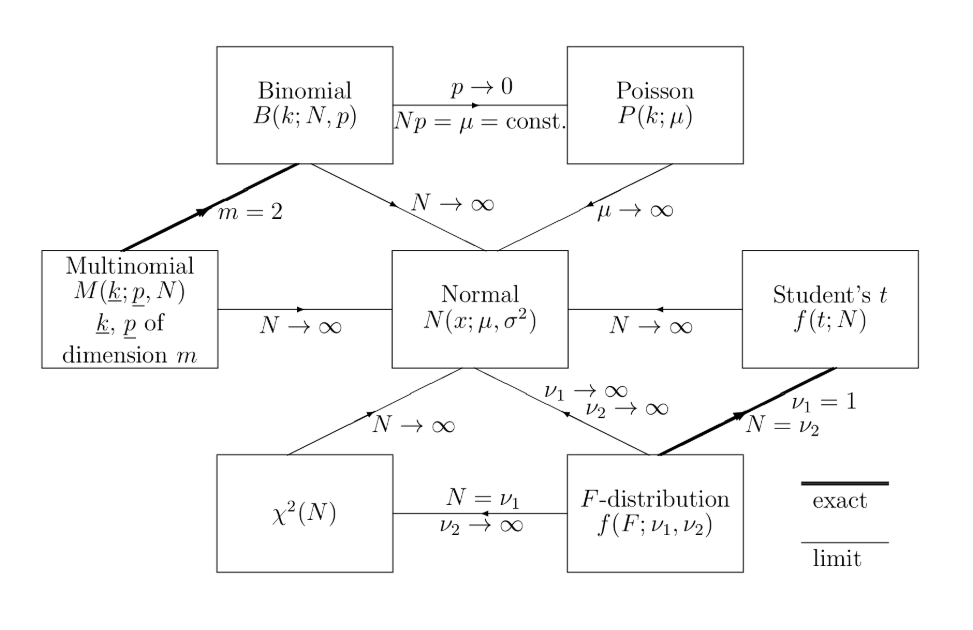
\includegraphics[scale = 0.4]{Asymptotic_map}	
\centering
\vspace{0.2in}
\caption{Mappa delle distribuzioni asintotiche}
\end{figure}


\section{Distribuzione di $\chi^2$}


La distribuzione di $\chi^2$ nasce nel contesto della modellazione di dati per la stima di parametri usando i metodi di maximum likelihood e minimi quadrati. Dato un campione di n punti $\{(x_i,y_i)\}_{i}^N$ e un modello $f(x, \bold{\underline{\theta}})$, dipendente da m parametri $\underline{\theta}$ si valuta la bont\`{a} del modello nell'approssimare i dati usando la funzione di $Q^2$ definita come:

\begin{equation}
	\chi^2 = \sum_{i=1}^{n}\dfrac{[y_i - f(x_i,\underline{\theta})]}{\sigma^2_i}
\end{equation}

dove le $\sigma^2_i$ sono gli errori sulle n misure di $y_i$. 
\newline
Per le misure y che seguono una pdf Gaussiana, la pdf del $\chi^2$ \`{e} data distribuzione:


\vspace{0.3in}

  \begin{minipage}{0.5\textwidth}
\begin{equation*}
	\chi^2 = \dfrac{1}{2^{\frac{n}{2}}\Gamma(\frac{n}{2})}z^{(\frac{n}{2}-1)}e^{-\frac{z}{2}}
\end{equation*}
  \end{minipage}
  \begin{minipage}{.4\textwidth}
    \centering
    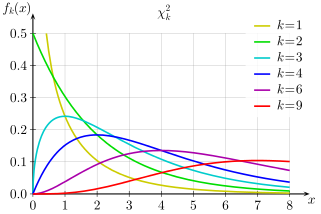
\includegraphics[scale = 0.545]{chi2.png}

  \end{minipage}
\vspace{0.3in}

dove \textbf{n} prende il nome di \textbf{numero di gradi di libert\`{a}} e $\Gamma(x)$ \`{e} la funzione gamma.

\begin{wrapfigure}[7]{l}{0.\textwidth}
\centering

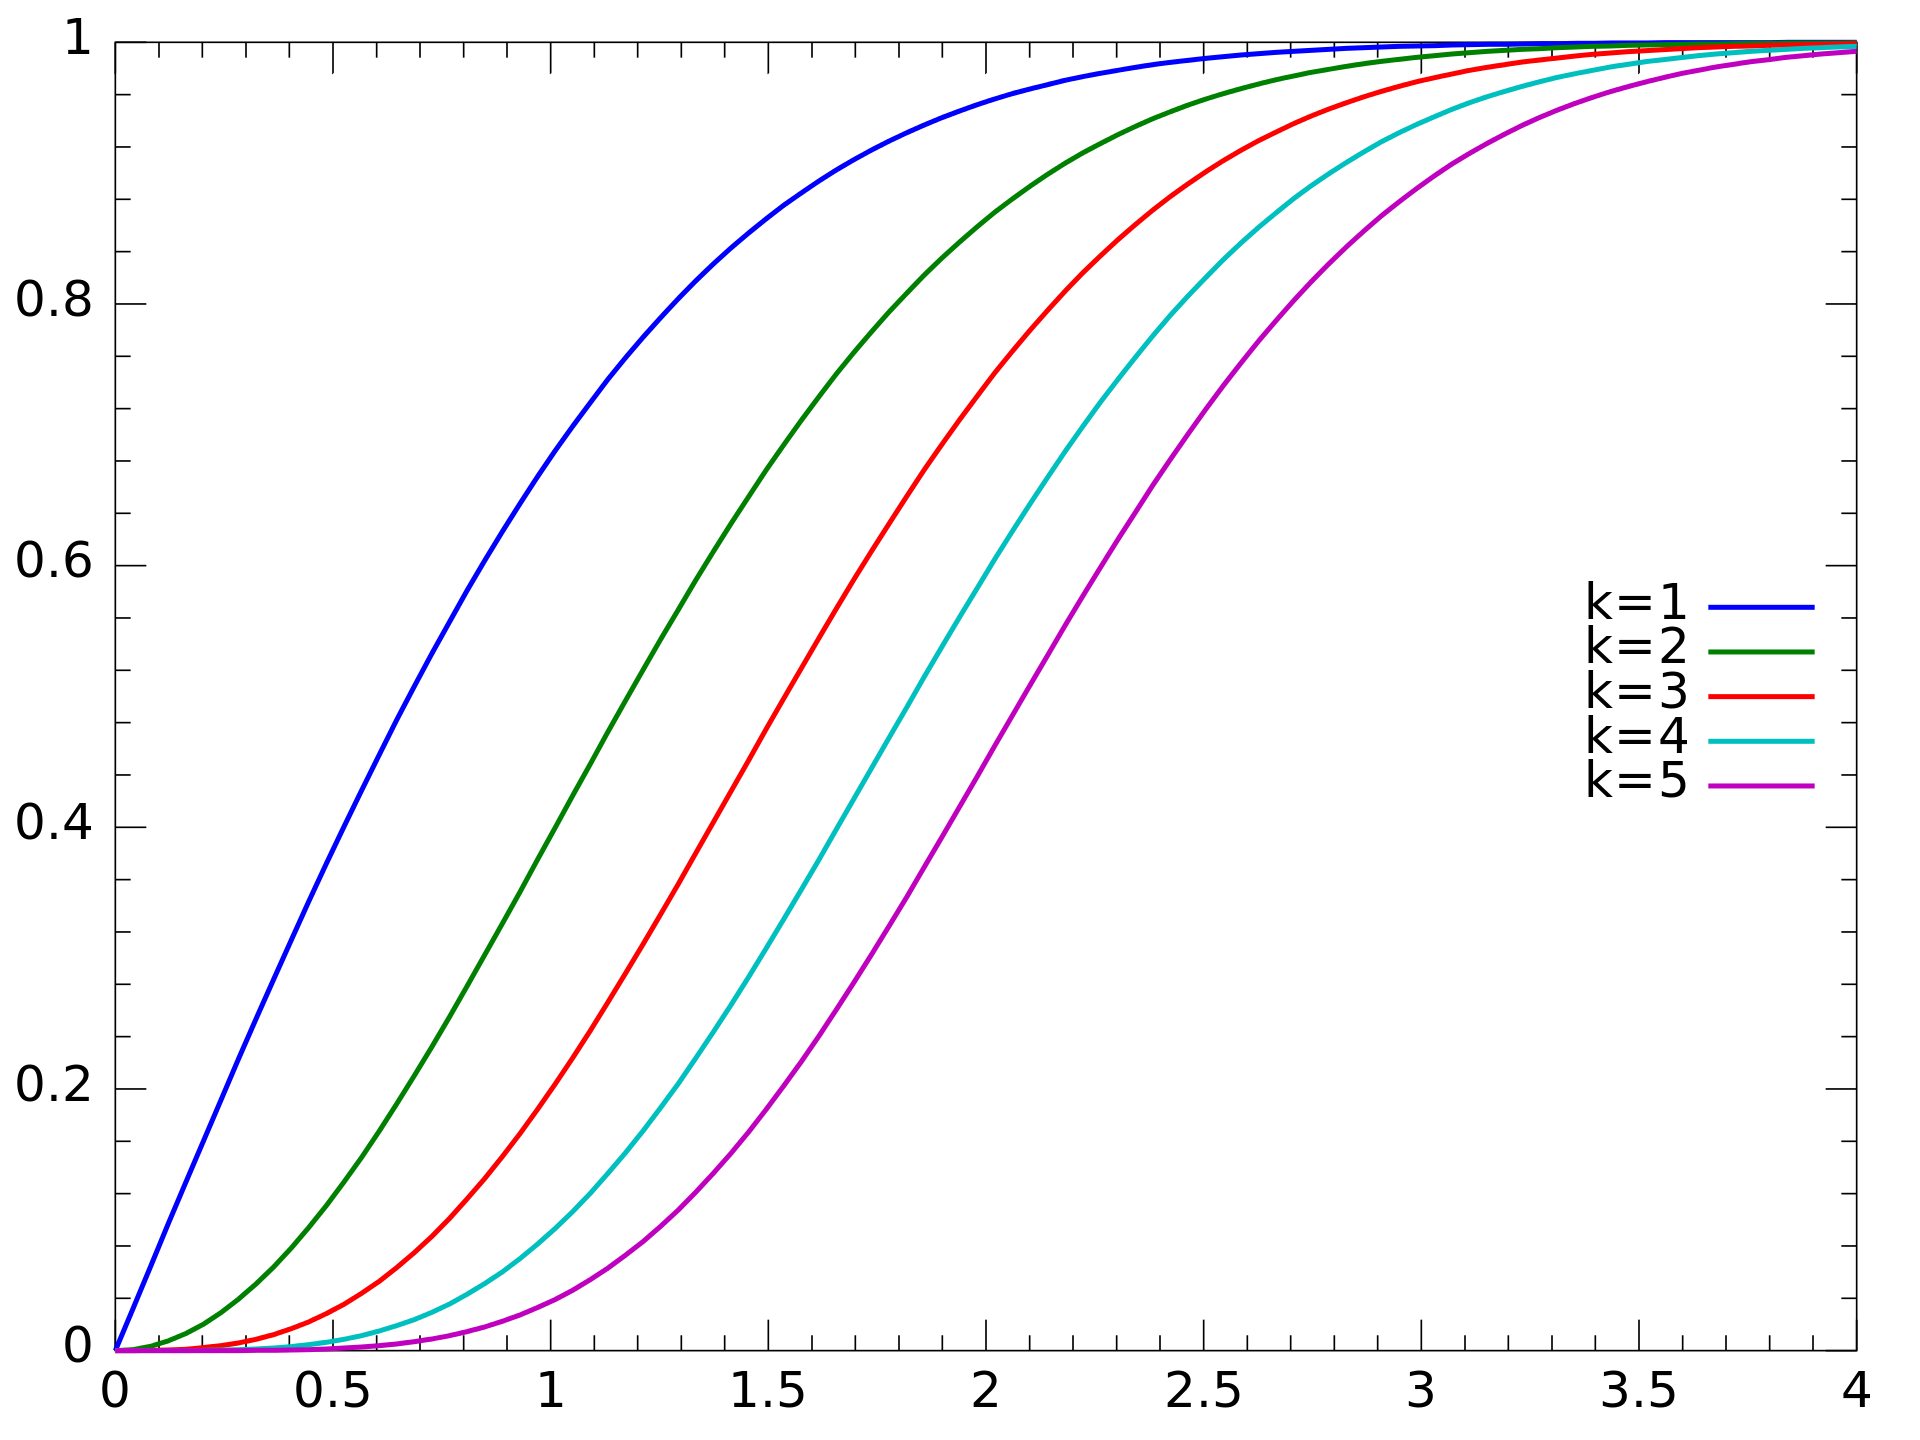
\includegraphics[scale = 0.1]{chiCdf.png}	

\end{wrapfigure}

\noindent La distribuzione di $\chi^2$ possiede una distribuzione cumulativa e gode delle seguenti propriet\`{a}:

\begin{itemize}
	\item \textbf{media:} E[n] = n
	\item \textbf{Varianza:} V[n] = 2n
	\item \`{e} riproduttiva
	\item \textbf{moda:} n-2
	\end{itemize}
	
\subsubsection{$\chi^2$ ridotto}

Si definisce $\chi^2$ ridotto data dal rapporto $\frac{\chi^2_N}{n}$ e la sua media \`{e} pari a 1.

 
\begin{figure}[ht]
\vspace{0.in}
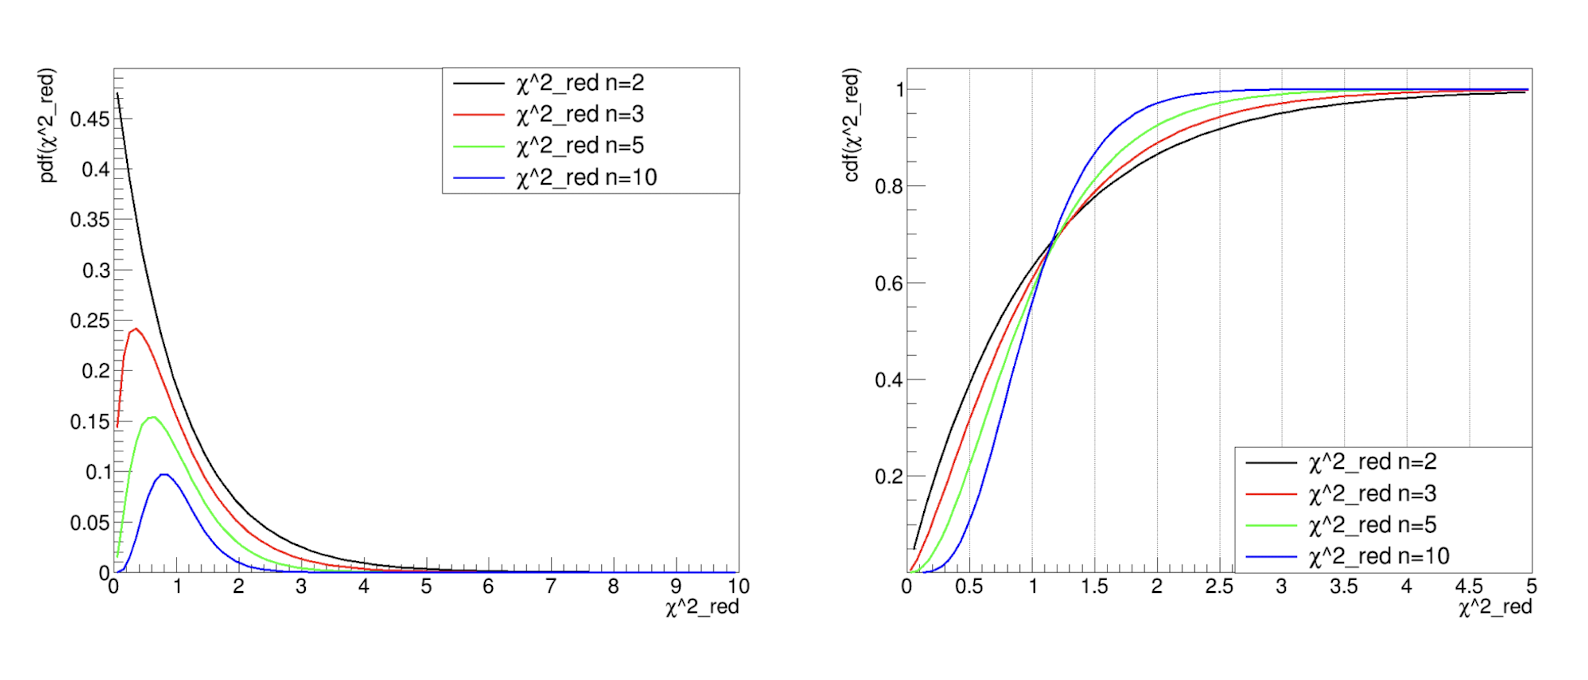
\includegraphics[scale = 0.5]{reducedChi}	
\centering
\vspace{0.in}
\caption{Distribuzione di $\chi^2$ ridotto e rispetti distribuzione cumulativa.}
\end{figure}

\vspace{0.05cm}
\par\noindent\rule{\textwidth}{2pt}

\section{Capitolo 2 - Guida allo studio}

\begin{enumerate}
	\item •	Che espressione analitica hanno e quali sono le proprietà notevoli delle distribuzioni uniforme, Gaussiana, lognormale?
	\item Che cosa sostiene il teorema centrale del limite?
	\item In particolare, quali sono le ipotesi nelle quali è valido?
	\item Quale è un contro esempio notevole che dimostra la necessità delle ipotesi?
	\item o	Che differenza c'è fra una distribuzione di densità di probabilità definita su dominio continuo ed una distribuzione di probabilità definita su dominio discreto?
	\item Come sono definite e quali sono le proprietà delle distribuzioni binomiale e di Bernoulli?
	\item Che applicazione notevole ha la distribuzione binomiale nell'interpretazione degli istogrammi di dati?
	\item Come sono definite e quali sono le propriet\'{a} della distribuzione di Poissoniana?
	\item Che ruolo hanno e come si utilizzano le distribuzioni Binomiale e Poissoniana nella lettura degli istogrammi che rappresentano la raccolta di misure?
	\item Come si applica il teorema centrale del limite alla distrubuzione di Poisson ed a quella binomiale?
	\item Quali sono le distribuzioni di probabilit\'{a} che caratterizzano i decadimenti radioattivi?
	\item In quali condizioni sono una buona rappresentazione delle misure?
	\item In quali circostanze \'{e} utilizzabile la distribuzione di Poisson nell'ambito delle misure di decadimenti radioattivi?
	\item Che legame c'\`{e} fra la distribuzione di Poisson e quella esponenziale?
	\item Che cosa \`{e} una distribuzione multinominale?
	\item Quali sono le propriet\`{a} della distribuzione del chiquadro?
\end{enumerate}


\setcounter{chapter}{2}
  	\chapter{Distribuzioni di probabilit\`{a} multidimensionali}
  	
  	\section{Probabilit\`{a} per variabili aleatorie in pi\`{u} \\ dimensioni}
  	
  	Quando un evento \`{e} identificato da un vettore $\underline{x}$, si parla di di distribuzioni di probabilit\`{a} multidimensionali o \textbf{joint pdf (probabilt\`{a} congiunta)}.  
  	
  	\begin{equation*}
  		pdf(\underline{x}): A \subseteq \mathbb{R}^n \rightarrow \mathbb{R}^+
  	\end{equation*}
  	
  	e la cdf per estensione della definizione mono-dimensionale \`{e}:
  	
	\begin{equation*}
  		cdf(\underline{x}) = \int_{A}pdf(\underline{x}) \cdot d\underline{x}
	\end{equation*}
  	
  	
	la probabili\`{a} di un evento per una variabile continua $\underline{x}$ \`{e} definita su una regione di spazio $A \subseteq \mathbb{R}^n$:
  	
	\vspace{0.2in}
  \begin{minipage}{0.5\textwidth}
		\begin{equation*}
  			P(\underline{x} \in A) = \int_{A}pdff(\underline{x}) \cdot d\underline{x}
  		\end{equation*}
  \end{minipage}
  \begin{minipage}{.4\textwidth}
    \centering
    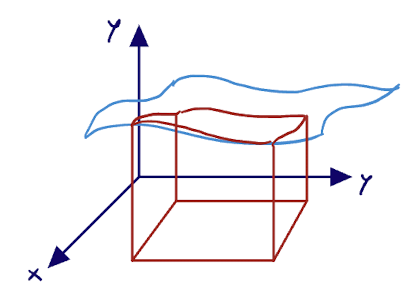
\includegraphics[scale = 0.42]{multi}

  \end{minipage}
	\vspace{0.2in}

Tale definizione di probabilit\`{a} verifica gli assiomi di Kolgomorov.
	
\section{Distribuzione di probabilit\`{a} marginale}

Data una distribuzione di probabilit\`{a} multidimensionale pdf($x_1,\cdots x_n)$ si definisce \textbf{distribuzione di probabilit\`{a} marginale}:

\begin{equation}
	f_{x_i}(x_1, \cdots,x_{i},\cdots,x_n) = \int pdf(x_1,\cdots,x_i,\cdots,x_n)dx_1\cdots dx_n
\end{equation}

 
\begin{figure}[ht]
\vspace{0.in}
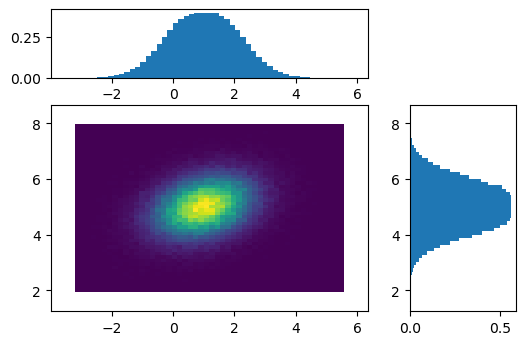
\includegraphics[scale = 0.6]{marginal.png}	
\centering
\vspace{0.in}
\caption{Distribuzione di probabilit\`{a} marginale per una pdf(x,y)}
\end{figure}

\subsubsection{Esempio}

Nel caso bi-dimensionale si ha che le rispettive distribuzioni marginali di una joint pdf$(x_1,x_2)$ sono date da:

\begin{equation}
	f_x(y) = \int pdf(x,y)dy \quad  \quad f_y(x) = \int pdf(x,y)dx
\end{equation}


\section{Distribuzione di probabilit\`{a} condizionata}

Per semplicit\`{a} consideriamo una distribuzione di probabilit\`{a} rispetto a due variabili aleatorie x ed y e le rispettive distribuzioni marginali $f_x$ e $f_y$. Vogliamo determinare la  probabilit\`{a} che $P(x \vert y = y_0)$ o $P(y \vert x = x_0) $. Consideriamo due eventi $A,B \subset \Omega$ disgiunti. Possiamo identificare le pdf come:

\begin{itemize}
	\item $P(A \cap B) \rightarrow $ joint pdf
	\item P(A) $\rightarrow$ pdf marginale
	\item $P(A|B) \rightarrow $ pdf condizionata
\end{itemize}

\noindent Definiamo L'evento A = $\{ y \; \vert \; x \in [x_0,x_0 +dx]\;,\; y \in \mathbb{R} \} $ e l'evento B = $\{ x \; \vert \; y \in [y_0,y_0 +dx]\;,\; x \in \mathbb{R} \} $. Le probabilit\`{a} associate ai singoli eventi sono P(A) = $f_x$ e P(B) = $f_y$. Mentre la probabilit\`{a} congiunta \`{e} $P(A \cap B) = \int pdf(x_0,y_0)dxdy$. 

Di conseguenza possiamo scrivere la probabilit\`{a} condizionata come:

\begin{equation}
	pdf(x \vert y = y_0) = P(A\vert B) = \dfrac{P(A \cap B)}{P(B)} = \dfrac{pdf(x,y_0)}{fx(y_0)}
\end{equation}

e analogamente:

\begin{equation}
	pdf(y \vert x = x_0) = \dfrac{pdf(x_0,y)}{f_y(x_0)}
\end{equation}

\section{Valore di aspettazione di una joint pdf}

Per una distribuzione di probabilit\`{a} congiunta abbiamo che il valore di aspettazione \`{e} definito da un vettore:
\begin{align}
E[\underline{x}] =
	\begin{bmatrix}
		\mu_x \\
		\mu_y \\
	\end{bmatrix}
	= 
	\begin{bmatrix}
		\int \int x \cdot pdf(x,y)dxdy \\
		\int \int y \cdot pdf(x,y)dxdy \\
	\end{bmatrix}	
\end{align}



\section{Varianza di una pdf multidimensionale}

Nel caso della Varianza, le componenti di una variabile aleatoria multidimensionale $\underline{x}$ possono essere legate tra loro, ovvero avere una relazione nel modo in cui variano, tale legame prende il nome di \textbf{covarianza}. Per due componenti $x_i$ e $x_j$ con $i \neq j$ si ha che: 

\begin{equation}
	\sigma_{i,j}^2 = E[(x_i - \mu_i)(x_j - \mu_j)] = E[x_ix_j] - E[x_i]E[x_j]
\end{equation}  	

\noindent mentre   	

\begin{equation}
	\sigma_{i,i}^2 = E[(x_i-\mu_i)^2]
\end{equation}
 
\noindent di conseguenza la varianza di una pdf($\underline{x})$ multidimensionale \`{e} rappresentata da una matrice che prende il nome di \textbf{matrice di covarianza} ed ha dimensione $n \times n$ nel caso $\underline{x}$ sia un vettore dimensione n.

\begin{equation}
	V[\underline{x}] = \begin{bmatrix}
		V[x_1] & \cdots \cdots	& Cov[x_1,x_n] \\
		\vdots & \ddots & \vdots \\
		Cov[x_n,x_1] & \cdots \cdots & V[x_n]
	\end{bmatrix}
\end{equation}
\newline

\noindent Nel caso in cui le componenti della variabile aleatoria $\underline{x}$ siano indipendenti tra loro si ha che la covarianza \`{e} nulla e dunque la (3.3) diventa una matrice diagonale.

\begin{equation}
	V[\underline{x}] = \begin{bmatrix}
		V[x_1] & \cdots \cdots	& 0 \\
		\vdots &\ddots & \vdots \\
		0 & \cdots \cdots & V[x_n]
	\end{bmatrix}
\end{equation}
\newline

La covarianza gode delle seguenti propriet\`{a}:
\begin{itemize}
	\item Avere $Cov[x_i,x_j] = 0 $ non implica necessariamente che le due variabili aleatorie siano statisticamente indipendenti.
	\item Se due variabili aleatorie sono statisticamente indipendenti \\ $\Rightarrow Cov[x_i,x_j] = 0 $
	\item Se due variabili aleatorie sono linearmente dipendenti \\$\Rightarrow Cov[x_i,x_j] = 0 $
	\item  La matrice di covarianza \`{e} simmetrica $\Rightarrow$ \`{e} diagonalizzabile.
\end{itemize}
 
 
\begin{figure}[ht]

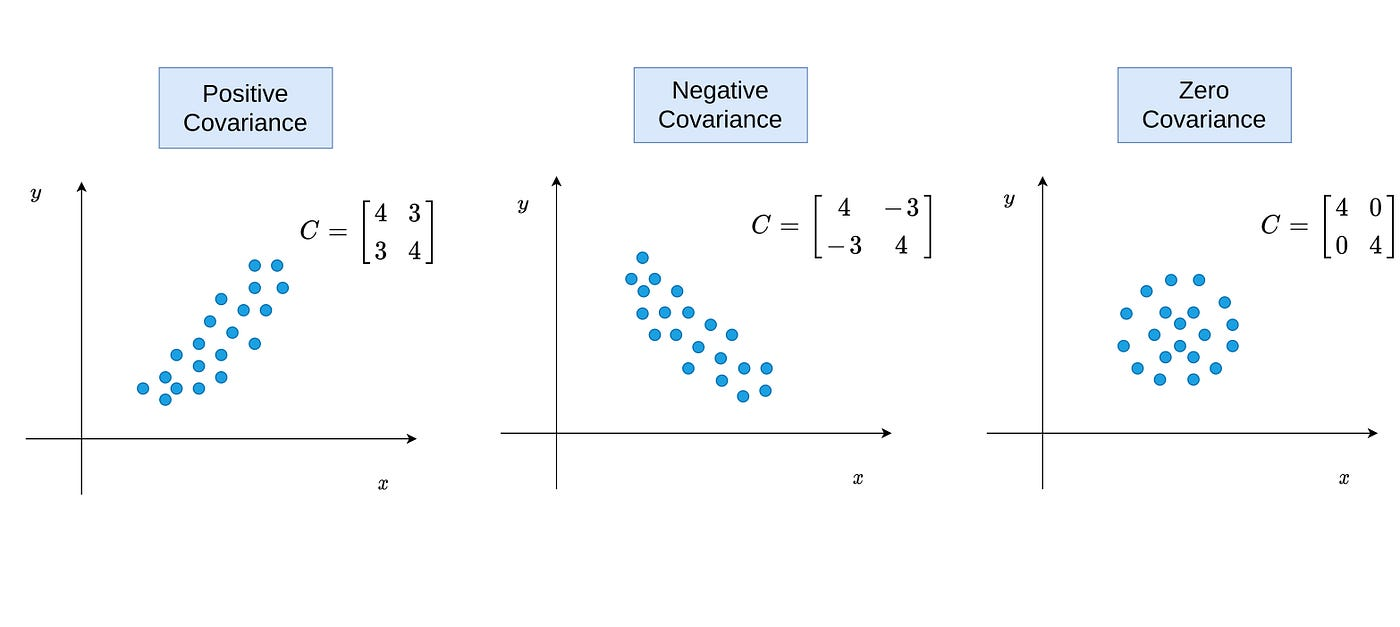
\includegraphics[scale = 0.23]{cov.jpeg}	
\centering
\caption{Esempi di come la covarianza si presenta in una distribuzione}
\end{figure} 

\section{Correlazione}
Gli elementi $V_{ij}$ della matrice di covarianza misurano il grado di correlazione tra le variabili $x_i$ e $x_j$. Dato che ogni variabili mostra una varianza finita e positiva \`{e} utile confrontare la covarianza  rispetto alle loro rispettive varianze, per farlo si introduce il coefficiente di correlazione:
\begin{equation}
	\rho_{ij} = \dfrac{Cov[x_i,x_j]}{\sigma_i \sigma_j}
\end{equation}

tale grandezza $\rho_{ij} \in [-1,1]$.

\begin{figure}[ht]
\vspace{0.2in}
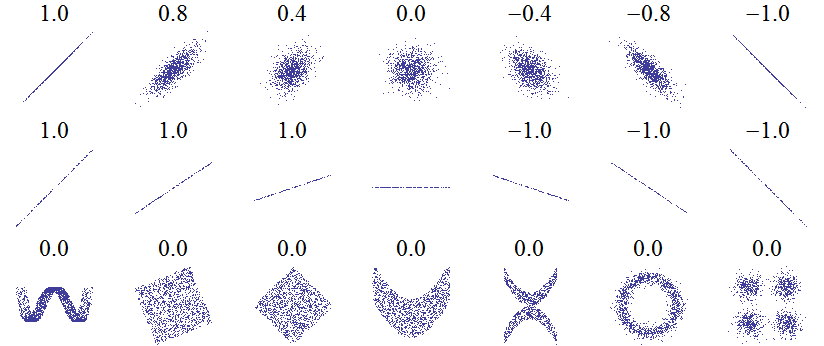
\includegraphics[scale = 0.45]{corre.png}	
\centering
\vspace{0.2in}
\caption{Indice di correlazione di Pearson per un campione di misure.}
\end{figure} 

\section{Variabili Statisticamente indipendenti}
Applichiamo la definizione di probabilit\`{a} congiunta data dall'equazione (3.3), poich\`{e} per ipotizziamo che  $P(x_2 \vert x_1)$ e $x_2$ non dipenda da $x_1$ avremo che:
\begin{equation*}
pdf(x_2 \vert x_1) = \dfrac{pdf(x_1,x_2)}{f_{x_1}} \Rightarrow pdf((x_1,x_2) = f_{x_1} \cdot pdf(x_2 \vert x_1)
\end{equation*}
si ha che  
\begin{equation*}
\quad f_{x_2}(x_1) = \int pdf(x_1,x_2)dx_1 = pdf(x_2\vert x_1) \int f_{x_1}dx_{1} = pdf (x_2 \vert x_1)
\end{equation*}
dunque si ha che:
\begin{equation*}
	pdf(x_1,x_2) = f_{x_1} \cdot f_{x_2}
\end{equation*}

\subsubsection{Definizione d'indipendenza}
Due variabili aleatorie $x_1$ ed $x_2$ descritte da una joint pdf($x_1,x_2)$ si definiscono \textbf{indipendenti} $\iff$ la joint pdf($x_1,x_2)$ = $pdf(x_1) \cdot pdf(x_2)$ dove $ pdf(x_1)$ e $pdf(x_2)$ coincidono con le marginali.

\subsubsection{Teorema}
Due variabili aleatorie $x_1$ ed $x_2$ descritte da una joint pdf($x_1,x_2)$ sono indipendenti $\Rightarrow$ la covarianza pu\`{o} essere scritta come:
\begin{equation}
	E[(x_1-\mu_{x_1})(x_2 - \mu_{x_2})] = E[(x_1-\mu_{x_1})] \cdot E[(x_2 - \mu_{x_2})]
\end{equation}
 
\section{Cambiamento di variabili per una pdf \\ multidimensionale}

La matrice della varianza (3.6) \`{e} diagonalizzabile, questo vuol dire che esiste un cambio di base che la diagonalizza, in fisica \`{e} equivalente ad avere un cambio di variabile. Sperimentalmente raccolto un campione di misure esiste sempre un cambio di variabile tale per cui la matrice di covarianza \`{e} diagonalizzabile. Anche se con un cambio di variabili le grandezze diventano decorrelate $Cov[x_i,x_j] = 0$ questo non vuol dire che siano statisticamente indipendenti.

Analogamente al caso mono-dimensionale per il cambio di variabili si ha che date delle funzioni:

\begin{align*}
	\begin{cases}
		x = u(\alpha,\beta)\\
		y = w(\alpha, \beta)
	\end{cases}
\end{align*}

la join pdf nelle nuove coordinate sar\`{a} data da:

\begin{equation}
	pdf(\alpha, \beta) = pdf(x,y) \cdot \vert detJ\vert
\end{equation}

dove J \`{e} la matrice Jacobiana associata alla trasformazione.
\subsection{Propagazione degli errori}

Ipotizziamo di avere un insieme di N misure $\{x_i\}_i^N$ e usiamo tali valori come componenti di un vettore $\underline{x} \in \mathbb{R}^N$, descritto da una pdf($\underline{x})$ di cui conosciamo $\underline{\mu}$ e matrice di covarianza $V[\underline{x}]$, vogliamo calcolare $y = u(\underline{x})$. Per Farlo approssimiamo u(\underline{x}) con un sviluppo di Taylor al primo ordine in un intorno di $\underline{\mu}$:

\begin{equation*}
	u(\underline{x}) \approx u(\underline{\mu})+ \nabla u\big \vert_{x = \mu}\cdot (\underline{x} - \underline{\mu})
\end{equation*}

\noindent Dunque i momenti della $pdf(\underline{y})$ sono:

\begin{itemize}
	\item E[y] = E[u($\underline{\mu}$)] + $\sum_{i =1}^{n} \dfrac{\partial}{\partial x_{i}}u(\underline{\mu})E[(x_i - \mu_{i})] = u(\underline{\mu}) $
	\item $\sigma_y^2 = E[y^2] - E[y]^2 = E[ (\underline{x} - \underline{\mu})^T H(u(\underline{x}))\big \vert_{x = \mu}(\underline{x} - \underline{\mu})] = \\ \\ =\sum_{i,j =1}^n \dfrac{\partial u(\underline{x})}{\partial x_i} \cdot \dfrac{\partial u(\underline{x})}{\partial x_j}\Big \vert_{x = \mu} \cdot V_{ij}$
\end{itemize}
\vspace{0.1in}
\noindent Per un caso bidimensionale l'incertezza su z = f(x,y) \`{e} data da:
\vspace{0.05in}
\begin{equation}
	\sigma_{z}^2 = \Big (\dfrac{\partial f(x,y)}{\partial x}\Big)^2 \Big \vert_{x =\mu}  \sigma_x^2 + \Big (\dfrac{\partial f(x,y)}{\partial y}\Big)^2\Big \vert_{x =\mu}  \sigma_y^2 + 2 \dfrac{\partial f(x,y)}{\partial x} \cdot \dfrac{\partial f(x,y)}{\partial y}\Big \vert_{x =\mu} Cov[x,y]
\end{equation}
\newpage

\subsection{Decorrelazione delle variabili}

Consideriamo un vettore $\underline{x}$ le cui componenti sono variabili aleatorie dipendenti tra loro. Poich\`{e} la matrice di covarianza \`{e} simmetrica possiamo definire una matrice $U$ che la diagonalizza $D[\underline{y}] = U^T V[\underline{x}]U$, tale matrice definisce un cambio di coordinate $\underline{y} = U\underline{x}$ dove le componenti di $\underline{y}$ risultano essere decorrelate tra loro.

\section{Distribuzione di Gauss Multidimensionale}

L'espressione di una Gaussiana in pi\`{u} dimensioni \`{e} data da:

\begin{equation}
	f(\underline{x} \; \big \vert \;  \underline{\mu},V) = \dfrac{1}{(2 \pi)^{\frac{n}{2}}detV^{\frac{1}{2}}} \cdot \exp{\Big [-\frac{1}{2} <(\underline{x} - \underline{\mu}),V^{-1}(\underline{x} - \underline{\mu})> \Big ]}
	\end{equation}
	
	
 
\begin{figure}[ht]
\vspace{0.1in}
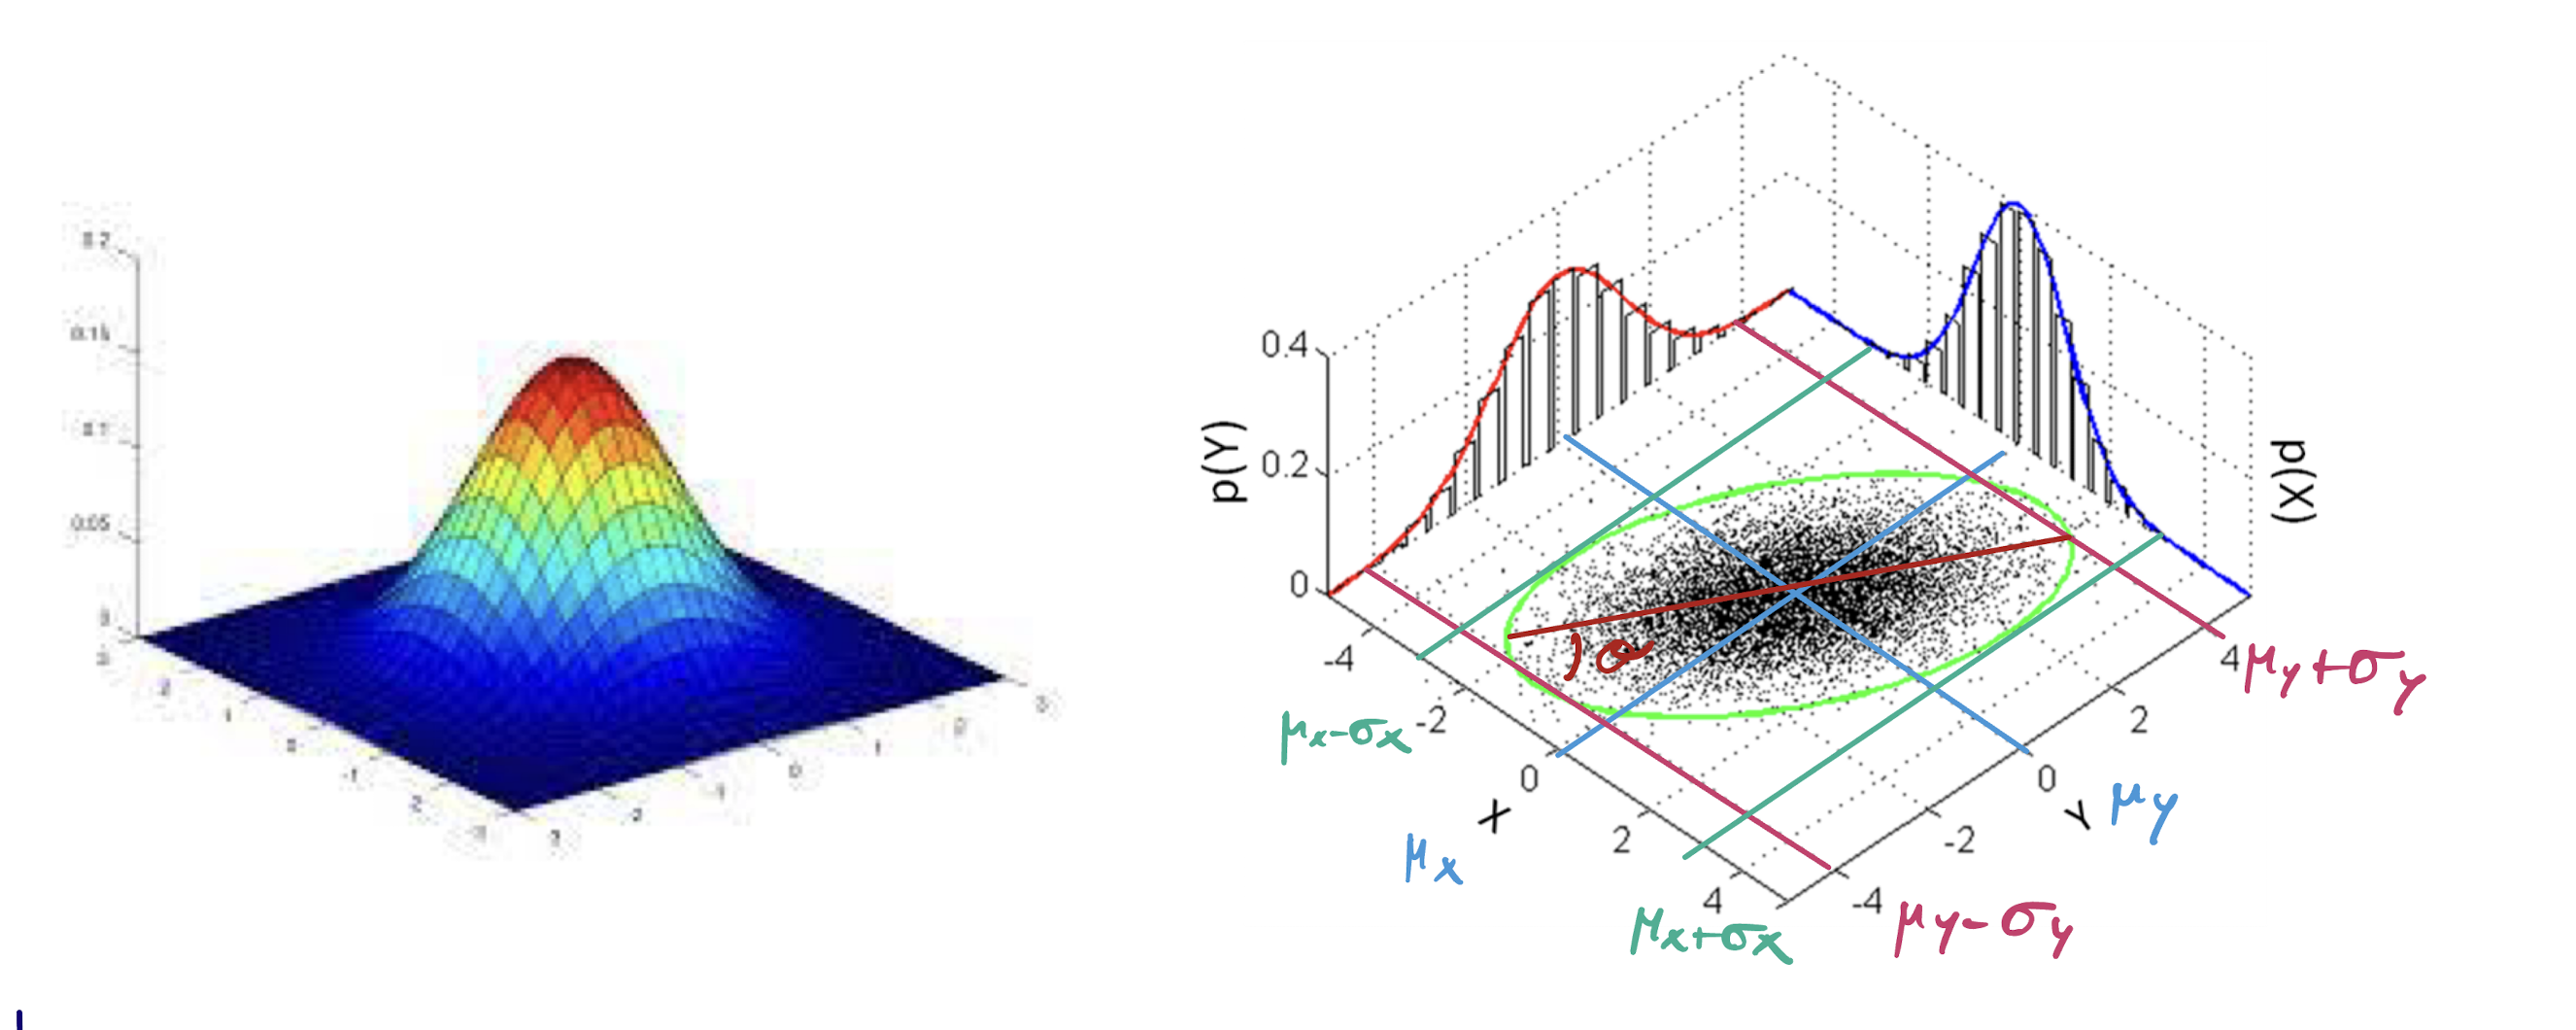
\includegraphics[scale = 0.3]{multiGauss}	
\centering
\vspace{0.1in}
\caption{Gaussiana in due variabili (x,y) e le sue distribuzioni marginali}
\end{figure}

\noindent La gaussiana in due dimensioni in generale ha un profilo ellittico per $1\sigma$. L'angolo d'inclinazione del semiasse maggiore \`{e} legato al coefficiente di correlazione:

\begin{equation}
	\theta = \dfrac{2\rho \sigma_x \sigma_y}{\sigma_x^2 - \sigma_y^2}
\end{equation}
\newline
Se esplicitiamo l'equazione (3.11) per due variabili si ha: 

\begin{align*}
	& f(x,y \; \big \vert \; \mu_x,\mu_y,V) = 
	\\
	\\
	&= \dfrac{1}{(2\pi)\sigma_x \sigma_y \sqrt{1-\rho^2}}  \exp{\Big \{ -\dfrac{1}{2(1-\rho^2)} \Big[ \Big ( \dfrac{x-\mu_x}{\sigma_x} \Big)^2 - \dfrac{2\rho(x-\mu_x)(y-\mu_y)}{\sigma_x \sigma_y} + \Big (\dfrac{y-\mu_y}{\sigma_y} \Big)^2  \Big]  \Big \}}	
\end{align*}
\newline
Se il coefficiente di correlazione di Pearson $\rho = 0$ possiamo riscrivere l'equazione precedente come:

\begin{align*}
	& f(x,y \; \big \vert \; \mu_x,\mu_y,V) = \dfrac{1}{(2\pi)\sigma_x \sigma_y} \exp{\Big \{ - \dfrac{1}{2} \Big[\Big ( \dfrac{x-\mu_x}{\sigma_x} \Big)^2 + \Big (\dfrac{y-\mu_y}{\sigma_y} \Big)^2 \Big] \Big \}} = 
	\\
	\\
	&\phantom{b= --------}= G(x,\mu_x,\sigma_x) \cdot G(y,\mu_y,\sigma_y)
\end{align*}
\newline
In generale \`{e} solo vero che due variabili statisticamente indipendenti sono anche decorrelate, nel caso Gaussiano vale anche il viceversa, ovvero se due variabili sono decorrelate allora sono anche statisticamente indipendenti.




\setcounter{chapter}{3}
\chapter{Stime di Parametri}


\section{La statistica}
La statistica studia il problema di inferire da un campione i parametri e/o i modelli che descrivono la popolazione dalla quale il campione \`{e} stato estratto. In particolare possiamo dividerla in due categorie:

\begin{itemize}
	\item Stima dei parametri, misura di una quantit\`{a} fisica;
	\item Test d'ipotesi, ovvero la prova della validit\`{a} di un modello.
\end{itemize}

Una funzione dipendente da N misure di un campione $f(x_1,...,x_n)$ si chiama \textbf{statistica}, essa \`{e} una \textbf{variabile aleatoria}. Quindi segue una sua distribuzione di probabilit\`{a} $pdf_f$ derivabile dalla joint-pdf dei campionamenti e dalla forma della funzione f.

\noindent Complessivamente si hanno 3 pdf:
\begin{itemize}
	\item la $pdf_x$(x,$\theta$) delle singole misure campionate; 
	\item la $pdf_{set}$($x_1,...,x_n,\theta)$ dei campionamenti (che \`{e} multidimensionale);
	\item la $pdf_f$ della statistica dei campionamenti (dipende dalla forma funzionale di f).
\end{itemize}


\section{Stimatori}

Sia data una p.d.f. (probability distribution function), $f(x,\theta)$ di una variabile x aleatoria  continua e dipendente da un parametro $\theta$, di cui non conosciamo il vero valore $\theta_{true}$.
\newline
Se si possiede un insieme $\{x_i\}_i^N$ di N misure della variabile x, possiamo chiederci se sia possibile determinare una stima del parametro $\theta_{true}$ in funzione di tali misure, $\hat{\theta} = \hat{\theta}(x_1,....,x_N)$, le funzioni di questo tipo prendono il nome di \textbf{stimatori}. Uno stimatore \`{e} una statistica opportunamente scelta. Con \textbf{stima} s'intende il valore assunto $\hat{\theta}^*$ dallo stimatore per uno specifico campione. 


\begin{figure}[ht]
\vspace{0.6in}

\includegraphics[scale = 1.3]{N_measure}	
\centering
\vspace{0.3in}
\caption{N misure}
\end{figure}

\noindent Poich\`{e} lo stimatore $\hat{\theta}$ \`{e} dipende da variabili aleatorie \`{e} anch'esso  una variabile aleatoria e dunque si pu\`{o} parlare di valore medio $E[\hat{\theta}]$ e varianza $V[\hat{\theta}]$ di una particolare stima, oltre ad avere una sua pdf$(\hat{\theta})$.

\begin{equation}
	\hat{\theta} \pm \sigma_{\theta}
\end{equation} 

Di conseguenza un insieme di misure restituir\`{a} un solo valore appartenente ad una popolazione ottenuta da campione fatto di misure della variabile aleatoria presa in considerazione.

\section{Propriet\`{a} degli stimatori}

Consideriamo un campione di N misure $\{x_i\}_i^N$ vengono definite IID (Independent Identically Distributed) quando sono:
\begin{itemize}
	\item \textbf{indipendenti:} l'esito di una misura non \`{e} influenzato dalle misure precedenti;
	\item \textbf{identiche:} Delle misure vengono definite identiche quando tutte quante seguono la stessa distribuzione di probabilit\`{a}
\end{itemize}
Nella statistica alle stime si possono associare diverse caratteristiche :

\begin{enumerate}
	\item \textbf{Consistenza:} una stima si dice consistente quando all'aumentare del numero di misure (convergenza probabilistica) si converge al valore vero del parametro. Ossia quando:
	\begin{equation}
		\lim_{N \rightarrow \infty} \hat{\theta}(x_1,.....,x_N) = \theta_{true} 
	\end{equation}
	 
\begin{figure}[ht]
\vspace{0.6in}
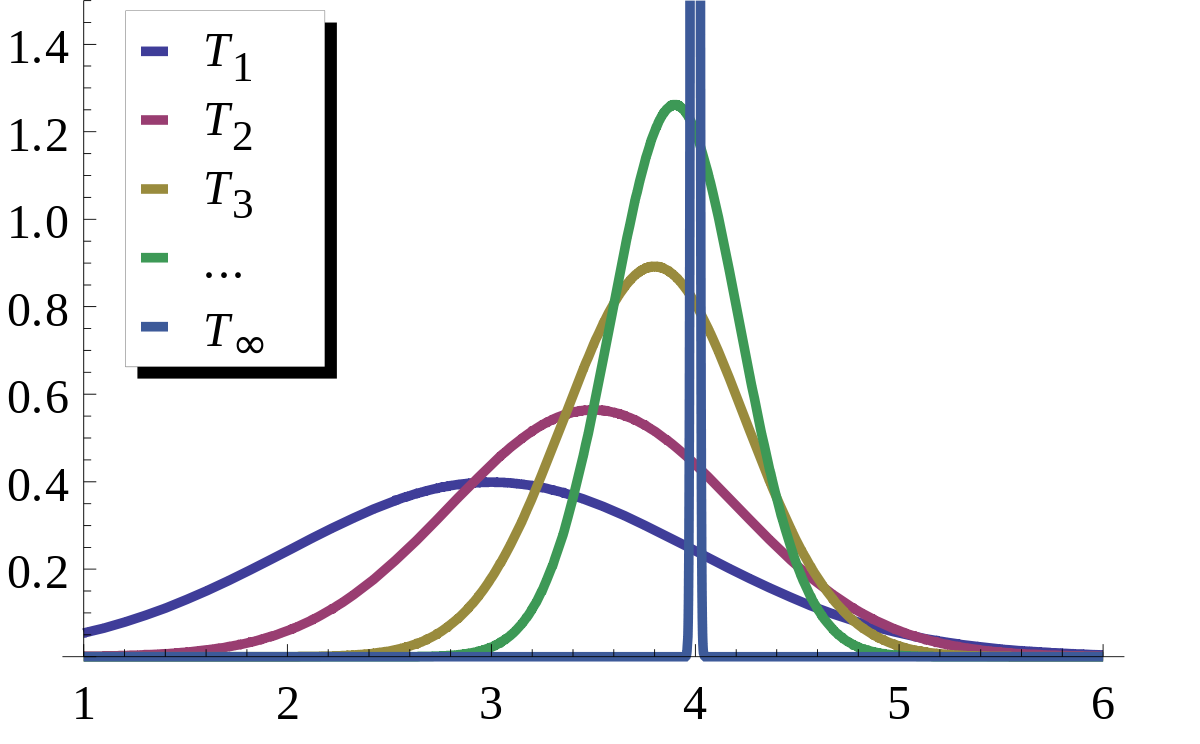
\includegraphics[scale = 0.2]{ConsistentEstimator}	
\centering
\vspace{0.3in}
\caption{Propriet\`{a} di consistenza di uno stimatore}
\end{figure}
	
	\item \textbf{Biased}: 
	\begin{enumerate}
	\item una stima si dice unbiased o imparziale, se mediamente coincide con il valore vero del parametro, ovvero 
	\begin{equation}
		b_{n}(\hat{\theta}) = E(\hat{\theta}_n - \theta_{true}) = E(\hat{\theta}_n) - E(\theta_{true}) = 0 
		\iff E(\hat{\theta_n}) = \theta_{true} 
	\end{equation}
	
	\item Una stima si dice asintoticamente unibiased se $b_n(\hat{\theta}) \rightarrow 0$ per $n \rightarrow \infty $.\newline
	\end{enumerate}
	Si osserva che $b_n{}(\hat{\theta})$ \`{e} uno stimatore lineare, dunque se $\hat{\theta}$ \`{e} stimatore di $\theta_{true}$ questo non vuol dire che $\hat{\theta}^2$ \`{e} stimatore di $\theta_{true}^2$.
	
	 
\begin{figure}[!ht]
\vspace{0.3in}
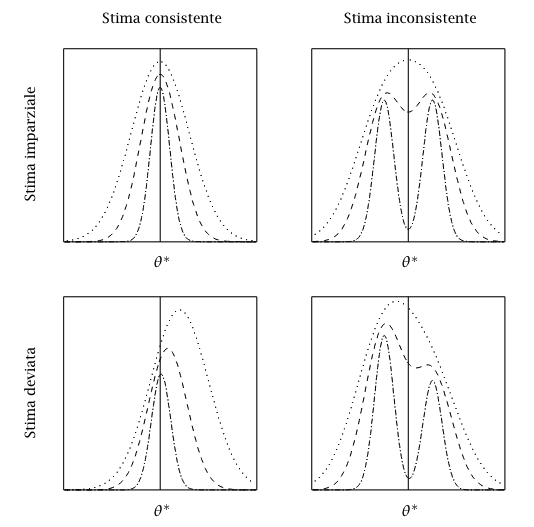
\includegraphics[scale = 0.5]{Stimatore}	
\centering
\vspace{0.3in}
\caption{Consistenza e Bias di uno stimatore}
\end{figure}
	
\item \textbf{Efficienza}: si dice che una stima \`{e} pi\`{u} efficiente di un'altra se la sua varianza \`{e} inferiore, quindi se mediamente essa \`{e} pi\`{u} vicina al valore centrale $E(\hat{\theta})$, che coincide con $\theta_{true}$ se la stima \`{e} anche imparziale (ubiased). 

\item \textbf{Varianza:} desideriamo che ripetendo i campionamenti le stime ottenute siano tutte vicine tra loro, ovvero la varianza della $pdf(\hat{\theta})$ sia il pi\`{u} piccola possibile.
\end{enumerate}

\subsection{Precisione e Accuratezza}

 Per uno stesso parametro si possono in generale definire tanti stimatori diversi tra loro, ma non tutti hanno le propriet\`{a} desiderate. Da notare che non \`{e} detto che esista (o sia possibile trovare) uno stimatore che soddisfi contemporaneamente tutte le propriet\`{a} richieste.
\subsubsection{Esempio} 

La media delle misure \`{e} uno stimatore non distorto. \newline

Dim.
\newline
Definito come stimatore la media aritmetica delle misure di un campione IID:
\begin{equation*}
		 \hat{\mu} = \frac{1}{N}\sum{x_{i}} 
\end{equation*}
si ha che il valore di aspettazione dello stimatore \`{e}:
\begin{equation*}
	  E(\hat{\mu})= E(\frac{1}{N}\sum x_{i})= \frac{1}{N}\sum E(x_{i})= \frac{1}{N} \cdot N \cdot \mu_{t} = \mu_{t} 
\end{equation*}
quindi la media aritmetica \`{e} uno stimatore \textbf{non distorto} poich\`{e}:
\begin{equation*}
	 b_n(\hat{\mu}) = E(\hat{\mu}) - \mu_{t} = \mu_{t} - \mu_{t} = 0  
\end{equation*}

\noindent Se la pdf(x) delle misure soddisfa le ipotesi del TCL, la pdf($\hat{\mu})$ per $N \rightarrow \infty$ tende a una \textbf{gaussiana} con media $\mu$ e varianza $\frac{\sigma^2}{N}$ si ha che $\hat{\mu}$ \`{e} uno stimatore \textbf{consistente}. Poich\`{e} $V[\hat{\mu}] = \frac{\sigma^2}{N}$ al crescere del numero di campionamenti la varianza si riduce e dunque le stime ottenute con diversi set di dati sono tutte vicine tra loro.


\subsection{Incertezze sulle stime}

\noindent Uno stimatore come ogni altra variabile aleatoria \`{e} soggetto a due tipi d'incertezze:

\begin{enumerate}
	\item \textbf{Incertezza sistematica:} nel caso di misure biased esiste una differenza sistematica fra la misura sperimentale ottenuta e il valor vero, ed \`{e} uguale per tutte le misure e non \`{e} possibile determinarlo essendo una propriet\`{a} intrinseca.
	\item \textbf{Incertezza statistica:} \`{e} associata alla precisione, e la si pu\`{o} ridurre aumentando il numero di misure o cambiando l'apparato sperimentale.
\end{enumerate}
\begin{equation}
		MSE =E[(\hat{\theta} -\theta_t)^2] =Var(\hat{\theta)} \: + \; b_{n}^2(\hat{\theta}) 
\end{equation}

Definisce l'errore quadratico medio e tiene conto sia dell'errore statistico misurato dalla varianza che dell'errore sistematico misurato dal bias.
\subsection{La Varianza come stimatore}

Consideriamo di avere un insieme di N misure, $\{x_{i}\}_{i}^N$ di cui conosciamo il valore medio $\mu$ della popolazione e di volerne determinare la varianza, poich\`{e} essa dipende dalle misure del campione \`{e} una variabile aleatoria a sua volta e dunque da un campione definiamo una stima del valore reale del parametro $\sigma_{t}$. Di conseguenza possiamo domandarci le propriet\`{a} che tale stimatore possiede.
	\newline
Definiamo lo stimatore varianza come:		
\begin{equation*}
		 \hat{\sigma}_{\mu}^2(x) = \frac{1}{N} \sum{(x_{i}-\mu})^2 \quad \text{oppure} \quad   \hat{\sigma}^2(x) = E(x^2) - E(x)^2
\end{equation*}

\noindent Verifichiamo che la varianza sia uno stimatore non distorto ovvero che:

\begin{equation*}
		E(\hat{\sigma}^2) = \sigma_{t}	
\end{equation*}

\noindent Per farlo sfruttiamo la porpriet\`{a} di linearit\`{a} del valore atteso.
\newline
Dim.
\begin{align*}	
		& E(\hat{\sigma}_{\mu}^2) = E(\frac{1}{N} \sum{(x_{i}-\mu})^2) = \frac{1}{N}\sum(E(x_i^2) - 2\mu E(x_i)+\mu^2) =
		\\
		\\
		 & = \frac{1}{N}\sum(E(x_i^2) - 2\mu E(x_i)+\mu^2) = \frac{1}{N}\sum(E(x_i^2) -\mu^2) = \frac{1}{N} \cdot N \cdot \sigma_t = \sigma_t
\end{align*}
\newline
\noindent Dunque la varianza \`{e} uno stimatore non distorto nel caso in cui si conosca il valore medio della popolazione. Raramente si conosce $\mu$ della popolazione, dunque consideriamo come stimatore la varianza per un campione di N misure IID.
\begin{equation*}
	\hat{\sigma}_{\overline{x}}^2 = \dfrac{1}{N}\sum_{i=1}^N(x_i - \overline{x})^2	
\end{equation*}
\newline
\noindent Sappiamo che la varianza determina la dispersione di un campione di misure attorno alla sua media. Ipotizziamo di conoscere il valore medio del campione $\overline{x}$, per costruzione risulta essere il valore pi\`{u} vicino alle misure dell'insieme. La media della popolazione $\mu$ non necessariamente coincide con $\overline{x}$ del campione, e dunque pu\`{o} non essere il valore attorno al quale si distribuiscono le misure del campione; infatti nel caso in cui non lo sia al crescere del numero di misure questo pu\`{o} diventare il valore pi\`{u} distante rispetto a $\overline{x}$ stimato dal campione iniziale. Le distanze quadratiche da  $\overline{x}$ saranno quindi una sottostima di $\mu$ e quindi anche $\hat{\sigma}$ sar\`{a} uno sottostima di $\sigma_t$.  
 \begin{align*}
		&E[\hat{\sigma}_{\overline{x}}^2] = \frac{1}{N} \sum{E(x_{i}^2}) - E([\frac{1}{N}\sum{x}_{i}]^2) = \sigma_{t}(x)^2 + \mu^2 - \frac{1}{N^2}[\sigma_{t}^2(\sum{x_{i}}) + E(\sum{x_{i}})^2] = 
		\\
		\\
		&= \sigma_{t}(x)^2 + \mu^2 - \frac{1}{N^2}[N\sigma_{t}^2(x) + N^2 \mu^2] = \sigma_{t}^2(x) \Big[\frac{N-1}{N} \Big ] 
\end{align*}
 
\noindent Di conseguenza la varianza di un campione $\hat{\sigma}_{\overline{x}}$ \`{e} uno stimatore distorto, infatti:
\begin{equation*}
	b_n[\hat{\sigma}_{\overline{x}}^2] = E[\hat{\sigma}_{\overline{x}}^2] - \sigma_{t}^2 = \sigma_{t}^2(x) \Big[\frac{N-1}{N} \Big ] - \sigma_{t}^2 
\end{equation*}
ma \textbf{asintoticamente non distorto} poich\`{e} per $N \rightarrow \infty $ si ha $b_n[\hat{\sigma}_{\overline{x}}^2] \rightarrow 0$.
\newline

\noindent Notare che quest'ultima definizione \`{e} quella operativa per verficiare che la varianza sia uno stimatore non ubiased in quanto difficilmente si conosce il valore medio $\mu$ della popolazione. 

\subsection{Correzione di Bessel}

Si pu\`{o} definire un terzo stimatore, che introduca una correzione a $\hat{\sigma}_{\overline{x}}^2$ tale da cancellare il bias. La correzione del bias \`{e} applicabile tutte le colte in cui il bias \`{e} precisamente noto. Il nuovo stimatore della varianza sar\`{a} dato da:

\begin{equation}
	s^2 \equiv \dfrac{1}{N-1} \sum_{i=1}^N (x_i - \overline{x})^2
\end{equation}
\newline
e prende il nome di \textbf{correzione di Bessel}.
\newline
Lo stimatore \`{e} unbiased $E[s^2] = \sigma_t^2$, ma la varianza di tale stimare non pu\`{o} essere determinata per il caso generale

\begin{equation*}
	V[s^2] = V[\dfrac{1}{N-1} \sum_{i=1}^N (x_i - \overline{x})^2] = \dfrac{1}{(N-1)^2} \sum_{i=1}^N V[(x_i - \overline{x})^2]
\end{equation*}
\newline
ma \`{e} possibile farlo solo nel caso in cui il campione di misura segue una pdf(x)\textbf{ Gaussiana}.
\begin{figure}[!ht]
\vspace{0.1in}
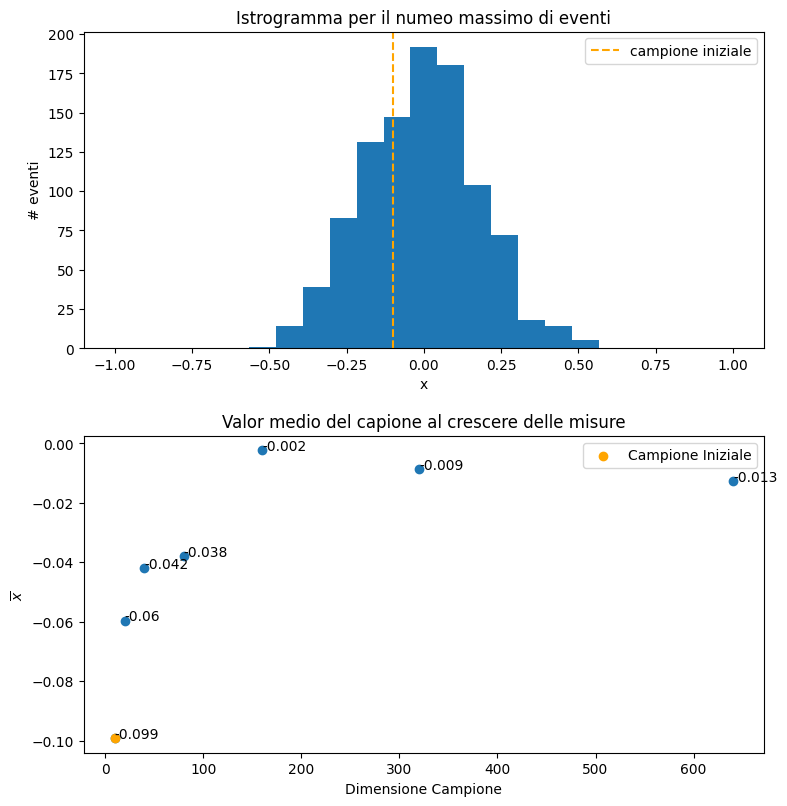
\includegraphics[scale = 0.5]{VarianceBiased}	
\centering
\vspace{0.3in}
\caption{Misure casuali che seguono una pdf di Gauss tra -1 e 1 in cui $\overline{x}$ del campione iniziale non coincide con il valore medio $\mu = 0$ della popolazione. Dunque $\overline{x}$ non \`{e} pi\`{u} il centro del campione al crescere delle misure. }
\end{figure}

\noindent Se riscriviamo lo stimatore $s^2$ nel seguente modo:

\begin{equation*}
s^2 \equiv \dfrac{1}{N-1} \sum_{i=1}^N (x_i - \overline{x})^2 = \dfrac{\sigma_t^2}{N-1} \textcolor{red}{\sum_{i=1}^N \dfrac{(x_i - \overline{x})^2}{\sigma_t^2}}
\end{equation*}
possiamo introdurre una variabile aleatoria ausiliaria definita come $\textcolor{red}{\chi^2}$ e riscrivere $s^2$ come:

\begin{equation*}
	s^2 \equiv \dfrac{\sigma_t^2}{N-1}\textcolor{red}{\chi^2}
\end{equation*}
\newline
di conseguenza $V[s^2]$ \`{e} legata alla $V[\textcolor{red}{\chi^2}]$. Nell'ipotesi in cui le misure raccolte seguano una distribuzione di probabilit\`{a} Gaussiana la variabile $\chi^2$ segue la distribuzione del chi-quadro. Tale pdf \`{e} descritta da un solo parametro definito gradi di libert\`{a} e nel nostro caso tale parametro vale N-1. 
\newline
Di conseguenza con questa nuova distribuzione possiamo dimostrare che $s^2$ \`{e} uno stimatore non distorto.\newline

Dim.

\begin{equation*}
	E[s^2] = E \Big[\dfrac{\sigma_t^2}{N-1}\textcolor{red}{\chi^2} \Big] = \dfrac{\sigma_t^2}{N-1}E[\textcolor{red}{\chi^2}] = \dfrac{\sigma_t^2}{N-1}(N-1) = \sigma_t^2
\end{equation*}
\newline
La sua varianza \`{e} data da:

\begin{equation*}
	V[s^2] = V \Big [ \dfrac{\sigma_t^4}{(N-1)^2}\textcolor{red}{\chi^2} \Big] = \dfrac{\sigma_t^4}{(N-1)^2}V[\textcolor{red}{\chi^2}] = \dfrac{2\sigma_t^4}{(N-1)^2} 
	\end{equation*}

\section{Intervallo di confidenza}

Si \`{e} costruito uno stimatore $\hat{\theta}$ per un parametro $\theta$ che \`{e} una variabile aleatoria di conseguenza esiste una distribuzione pdf($\hat{\theta}$) che \`{e} caratterizzata da una media E[$\hat{\theta}$] e una varianza V[$\hat{\theta}$]. La \textbf{stima} \`{e} il valore che lo stimatore assume in corrispondenza di un campione di dati e lo definiamo $\hat{\theta}^*$.\newline

\noindent L'\textbf{intervallo di confidenza} \`{e} solitamente indicato come:
\begin{equation}
	\hat{\theta}^* \pm \sigma \quad \text{oppure} \quad \hat{\theta}^* \; \begin{matrix}
		+\sigma_1 \\ - \sigma_1
	\end{matrix}
\end{equation}
la seconda notazione viene usata quando l'intervallo \`{e} asimmetrico. \newline
\begin{wrapfigure}{r}{0.5 \textwidth}

\vspace{-10pt}
\centering
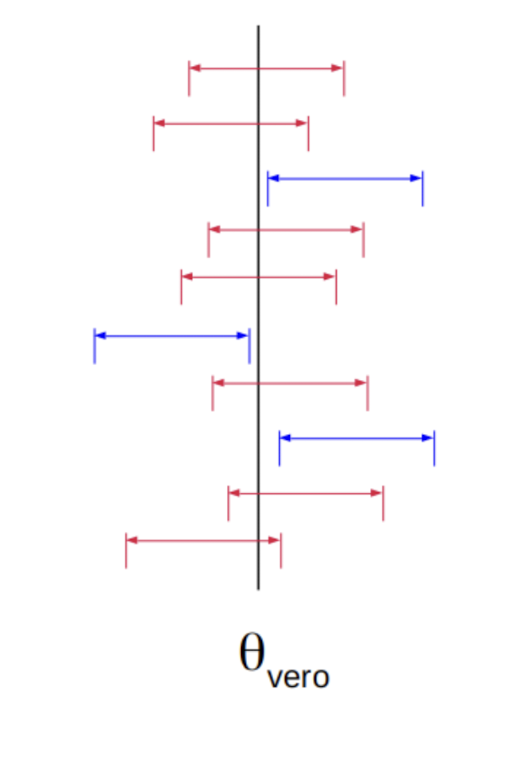
\includegraphics[width = 0.4 \textwidth]{interval}	

\end{wrapfigure}
In generale il risultato della stima \`{e} un intervallo [a,b], poich\`{e} \`{e} una variabile aleatoria si ha che gli estremanti sono variabili aleatorie e dunque per diversi campioni si hanno diversi intervalli di confidenza. A ciascun intervallo viene associata una probabilit\`{a} (\textbf{livello di confidenza}) che misura quanto \`{e} buona la stima del valore vero.

\begin{equation*}
	P(\theta_t \in [a,b])
\end{equation*}
dove essa rappresenta la frazione delle volte in cui ripetendo l'esperimento, la stima restituisce un intervallo che contiene il valore vero.\newline

In generale si vuole trovare un metodo che individui un intervallo [a,b] tale per cui la probabilit\`{a} che $\theta_t \in [a,b]$ sia pari a un certo valore $\beta$ detto \textbf{livello di confidenza}. Un intervallo di confidenza cos\`{i} definito prende il nome di \textbf{intervallo di condifenza di Neyman}. Un intervallo particolare \`{e} quello dato da $[\hat{\theta}^* - \sigma, \hat{\theta}^* + \sigma]$ e si definisce \textbf{intervallo centrale}.

\vspace{0.5cm}
\par\noindent\rule{\textwidth}{2pt}

\section{Capitolo 4 - Guida allo studio}

\begin{enumerate}
	\item Che cosa \`{e} una statistica?
	\item Che cosa \`{e} uno stimatore?
	\item Che cosa \`{e} uno stimatore consistente?
	\item Che cosa \`{e} la distorsione - o bias - di uno stimatore?
	\item Che propriet\`{a} hanno la media campionaria e la varianza di un campione, come stimatori di valore di aspettazione e varianza della popolazione?
	\item Che legame c'\`{e} fra la varianza di un campione di misure e la distribuzione del chiquadro?
	\item Quale \`{e} la varianza dello stimatore della media e della varianza di una misura?
	\item Che cosa \`{e} un intervallo di confidenza?
	\item Come si interpreta statisticamente?

\end{enumerate}


\setcounter{chapter}{4}
\chapter{Maximum Likelihood e Minimi Quadrati}

\section{La Verosomiglianza - Likelihood}

Date N misure  $\{x_{i}\}_{i}^N$ queste si definiscono IID quando sono:
\begin{itemize}
\item \textbf{indipendenti:} l'esito di un campionamento non \`{e} influenzato da nessuno degli altri
\item \textbf{identicamente distribuiti:} Tutte le misure seguono la stessa funzione di distribuzione di pobabilit\`{a}
\end{itemize}
\begin{equation*}
		pdf_x(x,\underline{\theta}): R \rightarrow R^+
\end{equation*}

\noindent La funzione di probabilit\`{a} congiunta (joint-pdf) di N campionamenti IID \`{e} il prodotto delle singole probabilit\`{a} (poich\`{e} indipendenti tra loro):

\begin{equation*}
		pdf_{set}(x_1.....,x_N,\underline{\theta}) = \prod_{i}^N pdf_{x}(x_i,\underline{\theta_{t}})	
\end{equation*}

\noindent essa rappresenta la densit\`{a} di probabilit\`{a} da associare all'evento casuale consistente nell'estrarre un particolare set di dati, ed \`{e} una funzione definita su uno spazio N-dimensionale.\newline

\noindent Se si sostituisce al valore vero $\underline{\theta_{t}}$ il generico valore $\underline{\hat{\theta}}$ stimato dalle N misure e se esse vengono considerate non pi\`{u} variabili casuali, ma costanti che sono state determinate dalle operazioni di misura, la precedente funzione prende il nome di \textit{funzione di verosomiglianza} o \textbf{likelihood}.

\begin{equation*}
		 L(\underline{x},\underline{\hat{\theta}}) = \prod_{i}^N pdf_{x}(x_i,\underline{\hat{\theta}}) 
\end{equation*}


\noindent Rappresenta la densit\`{a} di probabilit\`{a} da associare all-evento casuale consistente nell'essere un certo $\underline{\hat{\theta}}$ il valore vero del nostro parametro, nell'ipotesi di avere gi\`{a} ottenuto un set di N misure.\newline

\noindent \`{E} possibile definire anche la \textbf{loglikelihood} ovvero:

\begin{equation*}
	 l(\underline{\theta})= \log(L(\underline{x},\underline{\hat{\theta}})) = \log(\prod_{i}^N pdf_{x}(x_i,\underline{\hat{\theta}})) = \sum_{i}^N \log(pdf_{x}(x_{i},\underline{\theta})
\end{equation*}

\section{Comportamento della likelihood}

\noindent Raccolte delle misure $\{x_{i}\}_i^N$ IID, la funzione di likelihood $L(\theta)$ restituisce la probabilit\`{a} che si aveva di raccogliere tale campione assunta la conoscenza del parametro $\theta$  (che per comodit\`{a} in questo capitolo assumiamo in una sola dimensione). 
\hspace{0.5in}

\begin{wrapfigure}{r}{0.\textwidth}
\centering

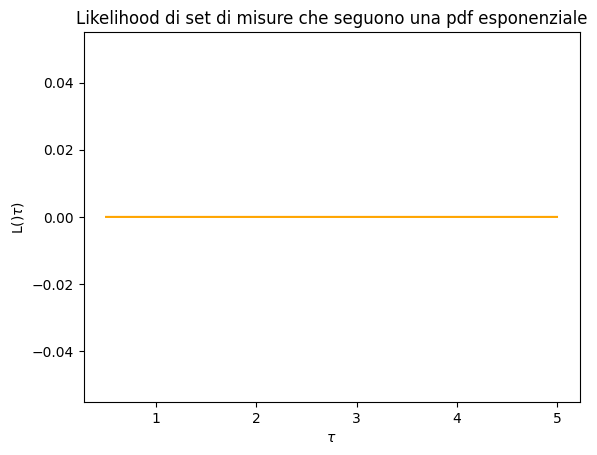
\includegraphics[scale = 0.4]{Like.png}	

\end{wrapfigure}

\noindent Se la $L(\theta)$ \`{e} all'incirca piatta vuol dire che  si ha la stessa probabilit\`{a} di ottenere un campionamento $\{x_1,....,x_N\}$ per ogni valore di $\theta$, ci\`{o} significa che i campionamenti non forniscono molte informazioni sul parametro $\theta$.  

\hspace{0.5in}


Se la $L(\theta)$ \`{e} una campana vuol dire si avr\`{a} una probabilit\`{a}:


\begin{wrapfigure}[5]{l}{0.5 \textwidth}

\vspace{-10pt}
\centering
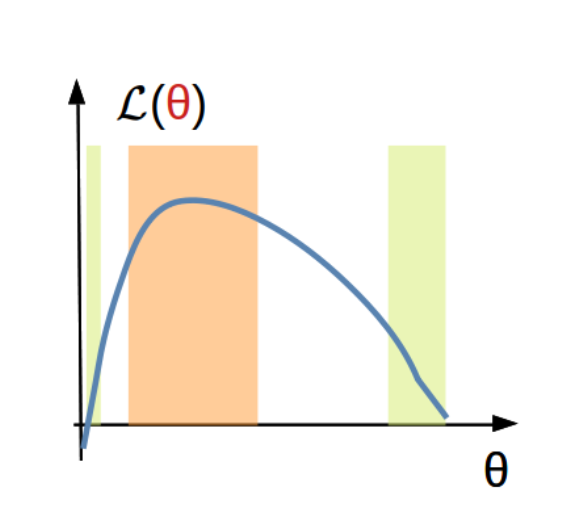
\includegraphics[width = 0.45 \textwidth]{loglike}	

\end{wrapfigure}

\noindent $\bullet \;$  Alta se il $\theta_{t}$ del campione \`{e} nell'area arancione in figura \\
\noindent $\bullet \;$ bassa se $\theta_{t}$ \`{e} nella regione verde \\
\noindent $\bullet \;$ massima se $\theta_{t}$ coincide con il massimo della funzione di likelihood \\
 
\noindent di aver raccolto il set di dati in esame. Dunque i campionamenti forniscono informazioni su $\theta$. Pi\`{u} \`{e} stretta la campana e pi\`{u} piccolo \`{e} il range dei valori che massimizzano la probabilit\`{a} di ottenere il campione raccolto. La larghezza della campana \`{e} legata all'incertezza con cui \`{e} possibile determinare il valore vero di $\theta$.
\newline

\noindent Quando definiamo una $pdf(x,\theta)$ senza conoscere $\theta$ si descrive un fascio di distribuzioni di probabilit\`{a} e dunque un'infinit\`{a} di modelli diversi. Cambiando la varianza di una distribuzione di cambia anche la funzione di likelihood.

\section{Minimum Variance Bound}

La funzione di likelihood $L(\theta)$ pu\`{o} essere utilizzata per misurare l'informazione che i campionamenti contengono relativamente al parametro $\theta$ che descrive il modello. L'informazione cos\`{i} ottenuta consente di valulatare la minima varianza  raggiungibile di uno stimatore di $\hat{\theta}$, ovvero dato un insieme di misure e un modello  esiste un limite inferiore  alla varianza raggiungibile.

\subsection{Informazione di Fischer}

Vogliamo costruire una metrica che $I ( \theta)$ che fornisca l'ammontare d'informazione contenuta in una variabile casuale osservabile x, relativamente a un parametro non osservabile $\theta$, da cui dipende la pdf(x). Tale funzione  prende il nome d'\textbf{informazione di Fischer}.

\begin{equation*}
		I(\theta) = E[(\frac{\partial}{\partial \theta}log(L(\theta)))^2] = -E[\frac{\partial^2}{\partial\theta^2}log(L(\theta)]
\end{equation*}

\noindent essa gode delle seguenti propriet\`{a}:

\begin{itemize}
	\item Associa un valore nullo se i dati sono irrilevanti per la stima di $\theta$.
	\item Aumenta al crescere della dimensione del campione ( purch\`{e} i dati siano rilevanti per la stima di $\theta)$.
	\item \`{E} legata alla precisione della stima: se l'informazione aumenta la varianza minima raggiungibile da uno stimatore $\hat{\theta}$ diminuisce.
\end{itemize}

\noindent Pi\`{u} i valori assunti dalla likelihood risultano essere sparpagliati peggiore \`{e} l'informazione che si ha a disposizione e dunque la precisione di stima di uno stimatore ne risentir\`{a} in egual modo. Viceversa pi\`{u} i valori risultano essere raggruppati in un certa regione di spazio e migliore sar\`{a} la precisione con cui si ottiene lo stimatore.

\subsection{Teorema di Rao - Cram\'{e}r}

Per uno stimatore $\hat{\theta}(x)$ consistente, bias $b_n(\hat{\theta})$, $V[\hat{\theta}] < \infty$ e non dipendente da x, definito su un dominio $\Omega_{\theta}$ si ha che il \textbf{MVB (Minimum Variance Bound)} definisce una relazione tra la varianza di un qualsiasi stimato $\hat{\theta}$ e la likelihood $L(\underline{X},\theta)$ nel seguente modo:

\begin{equation}
	V[\hat{\theta}] \geq \frac{(1-\frac{\partial}{\partial \theta}b_n(\theta))^2}{E[(\frac{\partial}{\partial \theta}log(L(\theta)))^2]} = V[\hat{\theta}]_{min}
\end{equation}
\newline
\noindent Al numeratore si ha una quantit\`{a} che dipende dallo specifico stimatore $\hat{\theta}$, ma solo se questo \`{e} biased, mentre a denominatore si ha l'informazione di Fischer, dunque una quantit\`{a} che non dipende dallo specifico stimatore ma solo da modello e dati.
\newline

\noindent Diciamo che uno stimatore \`{e} \textbf{efficiente} se la grandezza:

\begin{equation}
	\xi(\hat{\theta}) = \frac{V[\hat{\theta}]_{min}}{V[\hat{\theta}]} = 1
\end{equation}
	
\section{Maximum Likelihood}

Considerato un campione di N misure IID, si definiscono stimatori di \textbf{Maximum Likelihood (ML)} dei parametri quei valori che massimizzano la funzione di likelihood. Data una likelihood differenziabile rispetto $\underline{\theta}$ e il cui punto di massimo non \`{e} ai margini del range dei parametri, gli stimatori $\underline{\hat{\theta}}$ sono dati dalla soluzione delle equazioni differenziali:

\begin{equation}
\frac{\partial L}{\partial \theta_{i}}=0 \;\;\; i = 1,....,N
\end{equation}

\noindent Se esiste pi\`{u} di un massimo, viene considerato il maggiore. \newline

\noindent Con questa definizione di ML si considera il valore dello stimatore in corrispondenza del quale la probabilit\`{a} associata al campionamento \`{e} la massima possibile.

\noindent Le propriet\`{a} degli stimatori ottenute con il metodo di ML valgono asintoticamente, ovvero con un numero sufficientemente elevato di misure. Alcune \textbf{propriet\`{a} notevoli} sono:

\begin{enumerate}
	\item Consistente
	\item Asintoticamente efficiente
	\item Asintoticamente non distorto
	\item Propriet\`{a} d'invarianza: $\hat{\theta}_{ML}$ stimatore di $\theta_{t} \Rightarrow g(\hat{\theta}_{ML})$ \`{e} stimatore di $g(\theta_{t})$.
\end{enumerate}

\subsection*{Esempio propriet\`{a} d'invarianza}

Consideriamo la distribuzione esponenziale $f(x,\tau) = \frac{1}{\tau}e^{\frac{-t}{\tau}}$ e si abbiamo N misure IID la likelihood rispetto a $\tau$ \`{e} $L(\tau) = \prod_{i}^N \frac{1}{\tau}e^{\frac{-t_{i}}{\tau}}$.
\newline

\noindent Applichiamo il metodo di ML alla loglikelihood di $\tau$, dunque si ha che:

\begin{equation*}
		\sum_{i}^N(-\frac{1}{\tau}+ \frac{t_{i}}{\tau^2}) = 0 \iff N = \sum_{i}^N \frac{t_{i}}{\tau} \iff \tau_{ML} = \frac{1}{N} \sum_{i}^Nt_{i}
\end{equation*}

\noindent Posto $\lambda(\tau) = \frac{1}{\tau}$ possiamo riscrivere la pdf come $f(x,\lambda)= \lambda e^{-\lambda t}$ data la sostituzione vogliamo verificare che $\lambda(\tau_{ML}) = \frac{1}{\tau_{ML}}$.\newline


\noindent Dim.

\begin{equation*}
		\frac{\partial l}{\partial \theta} = 0 \iff \sum_{i}^N(\frac{1}{\lambda} - t_{i}) = 0 \iff \frac{N}{\lambda} = \sum_{i}^N t_{i} \iff \lambda = \frac{1}{\tau}
\end{equation*}

\noindent Se si dimostra che $\hat{\tau}$ \`{e} uno stimatore non distorto, \`{e} anche vero che $\hat{\lambda}$ \`{e} anch`esso non distorto ? \newline

Poich\`{e} la relazione $\hat{\lambda}(\hat{\tau})$ pu\`{o} essere non lineare non \`{e} detto che anche $\hat{\lambda}$ sia non distorto. 

\noindent Si pu\`{o} dimostrare che $\hat{\lambda}$ \`{e} uno stimatore distorto di $\lambda$ e dunque solo asintoticamente non lo \`{e}.

\section{Varianza dello stimatore di ML - Metodo Grafico}

Espandiamo fino al secondo ordine con un polinomio di Taylor la loglikelihood in un'intorno del parametro $\hat{\theta}$ ottenuto con il metodo di ML.

\begin{equation}
	log(L(\theta)) \approx log(L(\hat{\theta})) + \frac{1}{2}\frac{d^2}{d\theta^2}(log(L(\theta))\vert_{\theta = \hat{\theta}} (\theta - \hat{\theta})^2
\end{equation}

\noindent Se assumiamo che lo stimatore sia unbiased (il che per le propriet\`{a} precedente asintoticamente pu\`{o} esserlo) ed efficiente si ha dal teorema di Rao-Cramer che il secondo addendo \`{e} equivalente a:

\begin{equation*}
		\frac{d^2}{d\theta^2}(log(L(\theta))\vert_{\theta = \hat{\theta}} = - \frac{1}{\sigma_{\hat{\theta}_{ML}}}
\end{equation*}

\noindent E dunque possiamo riscrivere l'equazione (8.6) come:


\begin{equation}
	log(L(\theta)) \approx log(L(\hat{\theta})) -\frac{1}{2\sigma_{\hat{\theta}_{ML}}} (\theta - \hat{\theta})^2
\end{equation}

\noindent Consideriamo un cambio di variabile da $\hat{\theta}$ a $\hat{\theta}\pm \sigma_{\hat{\theta}}$ dunque possiamo riscrive la (8.7) come:

\begin{equation}
	log(L(\hat{\theta}\pm \sigma_{\hat{\theta}}) = log(L(\hat{\theta})) - \frac{1}{2}
\end{equation}

\noindent dunque da tale cambia di variabile si ha che la loglikelihood diminuisce della met\`{a} del suo valore di massimo. Si pu\`{o} dimostrare che la funzione di loglikelihood diventa una parabola (e la funzione di likelihood diventa una Gaussiana) per valori grandi del campione. Anche se la log(L) non \`{e} parabolica si pu\`{o} utilizzare l'equazione (8.8) come la definizione di errore statistico. Determinando i punti d'intersezione con quanto definito in (8.8) si ottiene una stima della varianza dello stimatore $\hat{\theta}$ usando il metodo di ML.

 
\begin{figure}[!ht]
\vspace{0.2in}
\includegraphics[scale = 0.32]{grafico}	
\centering
\vspace{0.2in}
\caption{funzione di loglikelihood, stima della varianza}
\end{figure}

\noindent Con un numero finito di misure l($\theta$) non \`{e} simmetrico e al crescere del numero di misure la forma funzionale assume un aspetto parabolico. Per simmetria la likelihood L($\theta$) diventa una Gaussiana.

 
\begin{figure}[!ht]
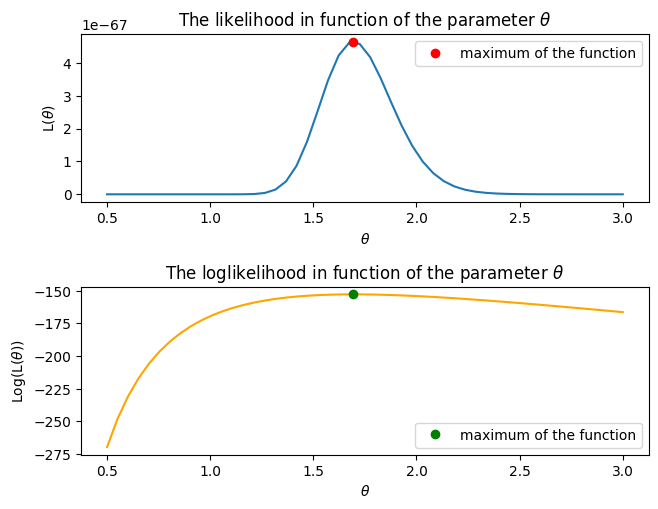
\includegraphics[scale = 0.45]{asinto}	
\centering
\caption{likelihood per un campione di 800 misure}
\end{figure}

\section{Extended likelihood}

Consideriamo una variabile aleatoria x distribuita secondo una pfd f(x,$\underline{\theta})$, dove i parametri $\underline{\theta}$ non li conosciamo e ipotizziamo di avere un campione di N misure $\{x_1,....,x_N\}$. Spesso si ha che il numero di osservazioni n del campione \`{e} una variabile aleatoria che segue una pdf Poissoniana con frequenza media $\lambda$. Il risultato di un'esperimento pu\`{o} essere definito dalla variabile n (che \`{e} la dimensione del campione) e dalle n misure raccolte $\{x_1,...,x_n\}.$ \newline
Dunque possiamo definire la likelihood dei parametri $\underline{\theta}$, dato un numero di venti medio $\lambda$ rispetto ad un campione di n misure.

\begin{equation}
	L(\lambda,\theta) = \dfrac{\lambda^{-n}}{n!}e^{-\lambda} \prod_{i=1}^nf(x_i,\underline{\theta}) = \dfrac{e^-{\lambda}}{n!} \prod_{i=1}^{n} \lambda_{i}f(x_i,\underline{\theta})
\end{equation}
Tale funzione prende il nome di \textbf{extended likelihood.}

\section{Varianza di uno stimatore per pi\`{u} parametri}

La varianza di $V[\hat{\theta}]$ di un vettore di parametri \`{e} definita dalla matrice di covarianza dove le sue componenti sono date da:

\begin{equation}
	V_{ij} = \Big[ - \dfrac{\partial^2}{\partial \theta_i \partial \theta_j}l(\hat{\theta}) \Big]^{-1} \quad \text{per} \quad i,j = 1,...,n
\end{equation}
dove i termini per $i \neq j$ sono dati da $Cov[\theta_i,\theta_j]$.
\section{Intervallo di confidenza}

Si \`{e} costruito uno stimatore $\hat{\theta}$ per un parametro $\theta$ che \`{e} una variabile aleatoria di conseguenza esiste una distribuzione pdf($\hat{\theta}$) che \`{e} caratterizzata da una media E[$\hat{\theta}$] e una varianza V[$\hat{\theta}$]. La \textbf{stima} \`{e} il valore che lo stimatore assume in corrispondenza di un campione di dati e lo definiamo $\hat{\theta}^*$.\newline

\noindent L'\textbf{intervallo di confidenza} \`{e} solitamente indicato come:
\begin{equation}
	\hat{\theta}^* \pm \sigma \quad \text{oppure} \quad \hat{\theta}^* \; \begin{matrix}
		+\sigma_1 \\ - \sigma_1
	\end{matrix}
\end{equation}
la seconda notazione viene usata quando l'intervallo \`{e} asimmetrico. \newline
\begin{wrapfigure}{r}{0.5 \textwidth}

\vspace{-10pt}
\centering
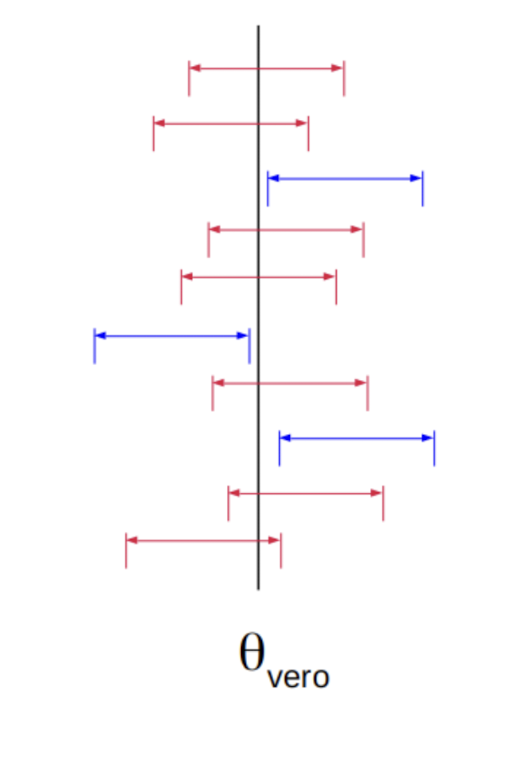
\includegraphics[width = 0.4 \textwidth]{interval}	

\end{wrapfigure}
In generale il risultato della stima \`{e} un intervallo [a,b], poich\`{e} \`{e} una variabile aleatoria si ha che gli estremanti sono variabili aleatorie e dunque per diversi campioni si hanno diversi intervalli di confidenza. A ciascun intervallo viene associata una probabilit\`{a} (\textbf{livello di confidenza}) che misura quanto \`{e} buona la stima del valore vero.

\begin{equation*}
	P(\theta_t \in [a,b])
\end{equation*}
dove essa rappresenta la frazione delle volte in cui ripetendo l'esperimento, la stima restituisce un intervallo che contiene il valore vero.\newline

In generale si vuole trovare un metodo che individui un intervallo [a,b] tale per cui la probabilit\`{a} che $\theta_t \in [a,b]$ sia pari a un certo valore $\beta$ detto \textbf{livello di confidenza}. Un intervallo di confidenza cos\`{i} definito prende il nome di \textbf{intervallo di condifenza di Neyman}. Un intervallo particolare \`{e} quello dato da $[\hat{\theta}^* - \sigma, \hat{\theta}^* + \sigma]$ e si definisce \textbf{intervallo centrale}.


\section{Metodo dei minimi quadrati}
Si parte da un modello $y = f(x,\underline{\theta})$ che definisce una relazione tra due grandezze fisiche x ed y e che dipende da N parametri $\underline{\theta}$, ipotizziamo di avere un campione di misure formato da punti $\{(x_i,y_i)\}_{i}^N$ ciascuno di essi segue una pdf(x) e una pdf(y) di conseguenza sono variabili aleatorie che hanno una loro incertezza $\sigma_x$ e $\sigma_y$. Vogliamo trovare un metodo che ci permetta di stimare i parametri ignoti partendo dai dati sperimentali. Tale metodo prende il nome di \textbf{interpolazione} o \textbf{fit} dei dati. Per semplicit\`{a} consideriamo il caso il cui l'incertezza sulle misure x sia trascurabile.

\subsection{Funzionale $Q^2$}

\noindent Partiamo considerando solo la variabile aleatoria x  e ci domandiamo per 
\begin{wrapfigure}{r}{0.5 \textwidth}
\vspace{-10pt}
\centering
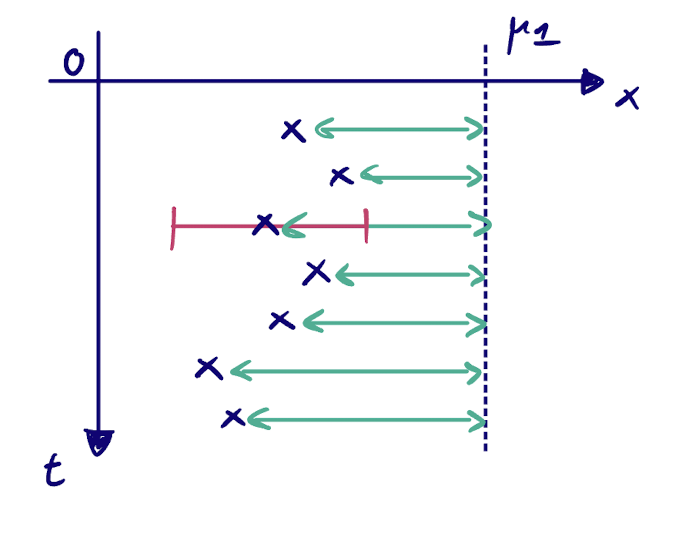
\includegraphics[width = 0.4 \textwidth]{q2}	
\end{wrapfigure}
quali valori del campione, si minimizza la distanza dalla media della popolazione $E[x] = \mu$; per rispondere a tale domanda definiamo la misura della distanza definendo un funzionale:
\newline

\begin{equation}
	Q^2\Big(\{x_i\}_1^N,\mu \Big) = \dfrac{1}{N}\sum_{i=1}^N\dfrac{(x_i - \mu)^2}{\sigma_i^2}
\end{equation}
\newline
Dunque ciascuna distanza \`{e} normalizzata alla larghezza della $pdf(x_i)$ e quindi tiene conto delle fluttuazioni statistiche di quel determinato campionamento.\newline
 Per determinare il  parametro cerchiamo quel valore $\hat{\mu}_{MQ}$ per cui $Q^2$ ammette un minimo assoluto nello spazio dei parametri (che nel nostro caso ha dimensione 1):

\begin{equation}
	\dfrac{d}{d\mu}Q^2 \Big(\{x_i\}_1^N, \mu \Big) = 0
\end{equation}
 

\subsection{Valore di aspettazione di $\hat{\mu}_{MQ}$}

Derivando la funzione di $Q^2$ si ha:

\begin{equation*}
	\dfrac{d}{d\mu}Q^2 = -2 \sum_{i=1}^N \dfrac{(x-\hat{\mu}_{MQ})}{\sigma_i^2} = 0 \iff  \hat{\mu}_{MQ} = \dfrac{\sum_{i=1}^N \frac{x_i}{\sigma_i^2}}{\sum_{i=1}^N \frac{1}{\sigma^2_i}}= \overline{x}
\end{equation*}

\noindent dunque per un campione di N misure la stima del valore atteso della popolazione coincide con la media aritmetica pesata del campione.

\subsection{Varianza dello stimatore $\hat{\mu}_{MQ}$}

Consideriamo $\hat{\mu}_{MQ} = \phi(x_1,....,x_N)$ e che il campione sia costituito da misure statisticamente indipendenti rispetto la variabile aleatoria x, la varianza dello stimatore sar\'{a} data da:

\begin{equation*}
	V[\hat{\mu}_{MQ}] = \sum_{i=1}^{N} \Big (\dfrac{\partial \phi}{\partial x_{i}} \Big)^2 \sigma_i^2 = \Big [\sum_{i=1}^N \frac{1}{\sigma^2_i} \Big ]^{-2} \sum_{i=1}^N \Big(\dfrac{1}{\sigma^2}\Big)^2 \sigma_i^2 = \dfrac{1}{\sum_{i=1}^N \frac{1}{\sigma^2_i}} < \sigma_i^2 \quad \forall i  
\end{equation*}
L'incertezza \`{e} dominata dalle misure con le $\sigma_{i}$ pi\`{u} piccole.

\section{Varianza di un stimatore usando i MQ - Metodo grafico}

Con il metodo di maximum likelihood si sono cercati i valori dei parametri che rendevano massima la probabilit\`{a}, dato un modello, di osservare i dati campionati. Con il metodo dei minimi quadrati invece si ceca il valore dei parametri che rende minima la distanza tra i dati campionati e il modello. Quando le $pdf(x_i)$ sono Gaussiane i due stimatori coincidono.

\begin{equation*}
	L(\hat{\theta}) = \prod_{i=1}^N \dfrac{1}{\sqrt{2\pi}\sigma_i}\exp{\Big [-\frac{ (x_i-\hat{\theta})^2}{2 \sigma_i^2} \Big]} = cost \cdot e^{-\frac{Q^2}{2}}
\end{equation*}
se passiamo alla loglikelihood

\begin{equation*}
	\log(L(\hat{\theta})) = \log(\text{cost}) - \dfrac{Q^2(\hat{\theta)}}{2}
\end{equation*}
Stimando $\hat{\theta}$ con il metodo di Maximum Likelihood si ha

\begin{equation}
	\dfrac{\partial \log(L(\hat{\theta}))}{\partial \hat{\theta}} = - \dfrac{1}{2}\dfrac{\partial Q^2(\hat{\theta})}{\partial \hat{\theta}}
\end{equation}
Quandole misure seguono una pdf Gaussiana e lo stimatore $\hat{\theta}$ \`{e} efficiente e non distorto sappiamo che il MVB coincide con la varianza dello stimatore ottenuto con il metodo di ML.

\begin{equation}
	V[\hat{\theta}_{ML}] = - \dfrac{1}{\dfrac{\partial^2 \log(L(\theta))}{\partial \theta^2} \Big \vert_{\theta = \hat{\theta}_{ML}}} 
\end{equation}
Dalla relazione (5.12) possiamo riscrivere l'uguaglianza (5.13) come:

\begin{equation}
	V[\hat{\theta}_{MQ}] = \dfrac{2}{\dfrac{\partial^2Q^2(\theta)}{\partial \theta^2} \Big \vert_{\theta = \hat{\theta}_{MQ}}}
\end{equation}
Sviluppando con Taylor al secondo ordine la funzione $Q^2$ in un intorno di $\hat{\theta}_{MQ}$ si ha:

\begin{equation*}
	Q^2(\theta) \approx Q^2(\hat{\theta}_{MQ}) + \dfrac{1}{2}\dfrac{d^2 Q^2(\theta)}{d\theta^2}\Big \vert_{\theta = \hat{\theta}_{MQ}}(\theta - \hat{\theta}_{MQ})^2 = Q^2(\hat{\theta}_{MQ}) + \dfrac{(\theta - \hat{\theta}_{MQ})^2}{V[\theta]}
\end{equation*}
Effettuando un cambio di coordinate $\theta = \hat{\theta}_{MQ} \pm \sigma_{\hat{\theta}}$ si ha:
\begin{equation*}
	Q^2(\hat{\theta}_{MQ} \pm \sigma_{\hat{\theta}}) = Q^2(\hat{\theta}_{MQ}) + 1
\end{equation*}
\begin{wrapfigure}[8]{r}{0.5 \textwidth}
\centering
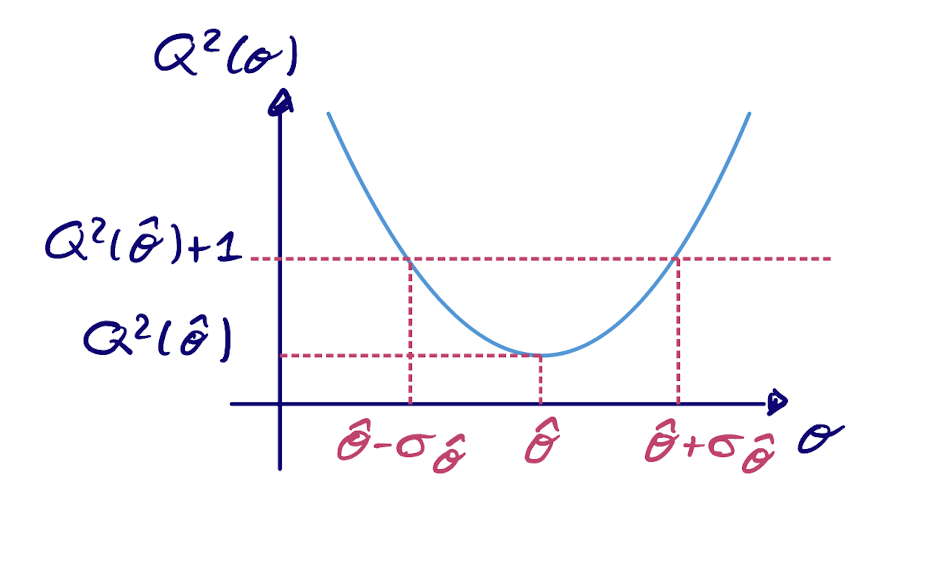
\includegraphics[width = 0.6 \textwidth]{graph}	

\end{wrapfigure}
\newline
Dunque considerando graficamente l'intersezione con $Q^2(\theta)$ si determinano $\hat{\theta}_{MQ} \pm \sigma_{\hat{\theta}}$. Poich\`{e} per ipotesi le misure $\{x_i\}_i^N$ seguono una distribuzione di probabilit\`{a} Gaussiana e sono IID si ha che $Q^2(\theta)$ segue la distribuzione di probabilit\`{a} del chi quadro $\chi^1(N-k)$ per E[$Q^2$] = N-k gradi di libert\`{a}. Se questo non avviene \`{e} perch\`{e}:
\begin{itemize}
	\item si \`{e} avuta una fluttuazione statistica sfavorevole
	\item il modello non descrive i dati
	\item il modello \`{e} corretto, ma i dati sono stati raccolti in modo errato
	\item il modello \`{e} corretto, ma le incertezze attribuite ai dati sono sbagliate (sono sopra o sottovalutate).
\end{itemize}

\section{Modelli lineari nei parametri}

Un modello si definisce \textbf{lineare} se due grandezza fisiche x ed y sono legate da una relazione lineare rispetto a parametr $\underline{\theta}$.

\begin{equation}
	y_{0}^{i} = \sum_{j = 1}^N \theta_{j}h_{j}(x_i)
\end{equation}
Assumiamo che l'incerteza sulla variabile x sia ininfluente, mentre y \`{e} una variabile aleatoria le cui misure sono IID con varianza $V[y_i] = \sigma_i^2$. Definiamo una variabile aleatoria asuiliaria $\epsilon$ che possiede la stessa distribuzione di probabilit\`{a} di y. Riscriviamo (5.15) come:

\begin{equation}
	y_i = \sum_{j = 1}^N \theta_{j}h_{j}(x_i) + \epsilon_i
\end{equation}
Assumiamo che per le $\epsilon$ valgano le seguenti propriet\'{a}:

\begin{equation*}
	E[\epsilon_i] = 0 \quad \quad V[\epsilon_i]= V[y_i] = \sigma_i^2
\end{equation*}
In questo modo la pdf(y) coincide con la pdf($\epsilon$). La variabile $\epsilon$ rappresenta l'errore statistico sulla misura, mentre le $y_0$ sono il valore vero della misura restituito dal modello.
\newline
Applichiamo il metodo dei minimi quadrati, andando a stimare quei valori dei parametri $\underline{\theta}$ che minimizzano la distanza tra il valore vero restituito dal modello lineare e i dati campionati sperimentalmente, pesando gli scarti quadratici rispetto la varianza delle distribuzioni di probabilit\`{a} delle singole $y_i$.

\newpage

 
\begin{figure}[ht]
\vspace{0.2in}
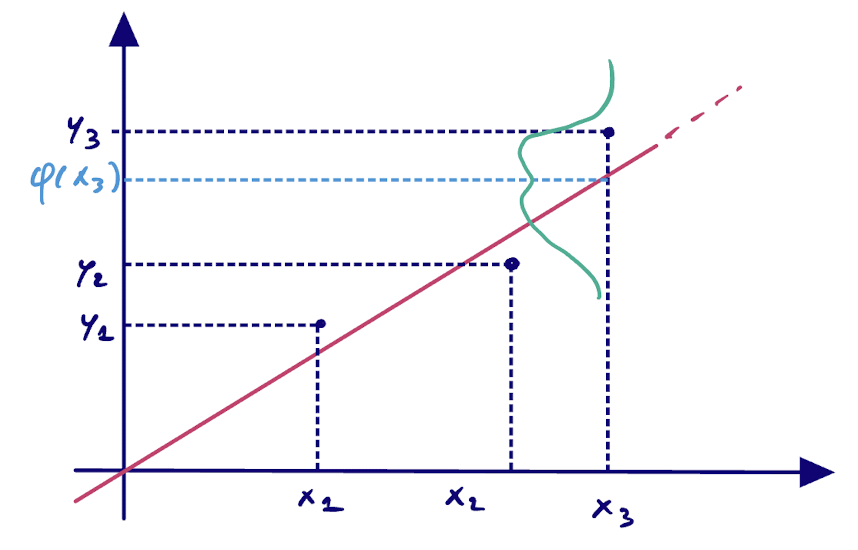
\includegraphics[scale = 0.5]{linear}	
\centering
\vspace{0.2in}
\caption{$\psi(x_3)$ rappresenta il valore vero della misura rispetto al modello, mentre $y_3$ il dato campionato su cui \`{e} presente un errore statistico.}
\end{figure}

\noindent Per farlo utilizziamo il funzionale $Q^2$ riscrivendolo come:

\begin{equation}
	Q^2 = \sum_{i=1}^N \dfrac{(y_i - y_0(x_i, \theta))^2}{\sigma_i^2} = \sum_{i=1}^N \dfrac{(y_i - \sum_{j=1}^N \theta_j h_j(x_i))^2}{\sigma_i^2} = \sum_{i=1}^N \dfrac{\epsilon_i}{\sigma^2_i} 
\end{equation}

\subsection{Stime dei parametri}

Per un vettore di parametri $\underline{\theta}$ di dimensione N, avremo un sistema di K equazioni:
\begin{align}
 \nabla Q^2(\underline{x},\underline{\theta}) =
	\begin{cases}
		\dfrac{\partial Q^{2}}{\partial \theta_{1}} = 0 \\
		\quad \vdots \\
		\dfrac{\partial Q^{2}}{\partial \theta_{n}} = 0 \\
	\end{cases} 
\end{align}
Per una singola riga si ha:
\begin{equation}
	\dfrac{\partial Q^{2}}{\partial\theta_{j}} = \sum_{i=1}^N \dfrac{-2}{\sigma^2_{j}} \Big ( \dfrac{y_i - \sum_{j=1}^N \theta_j h_j(x_i)}{\sigma_i} \Big )^2h_j(x_i) = 0 \quad \forall i = 1,...,N
\end{equation}
\newline
\noindent Per comodit\`{a} di esposizione riscriviamo l'espressione (5.16) in forma vettoriale:
\begin{equation}
	\underline{y} = H \underline{\theta} + \underline{\epsilon}
\end{equation}
ed essendo una modello a pi\`{u} parametri si ha la matrice di covarianza $V[\epsilon]$, possiamo considerare la matrice in funzione di $\epsilon$ poich\`{e} V[y] e $V[\epsilon]$ sono legate da una traslazione rigida e dunque risultano essere identiche. In generale tale matrice non \`{e} diagonale, ma poich\`{e} si \`{e} assunto che le misure siano IID la matrice \`{e} diagonale.
\begin{align*}
V[\epsilon] = 
\begin{bmatrix}
	\sigma_i^2 & \cdots\cdots & 0 \\
	\vdots & \ddots & \vdots \\
	0 & \cdots & \sigma_n^2
	\end{bmatrix}
\end{align*}
Riscrivendo $Q^2 = \underline{\epsilon}^TV^{-1}\underline{\epsilon}$ in forma matriciale e risolvendo il sistema (5.19) si stimano i parametri come:
\begin{equation}
	\underline{\hat{\theta }}_{MQ} = (H^TV^{-1}H)^{-1}\cdot H^TV^{-1}\underline{y}
\end{equation}
dove $V(\underline{\hat{\theta}}) = (H^TV^{-1}H)^{-1}$ dove nella matrice H \`{e} contenuta l'informazione delle misure.\newline
\noindent Resta da verificare che lo stimatore sia non distorto ovvero $E(\underline{\hat{\theta}}) = \underline{\theta}_t$:
\begin{equation*}
	E[\hat{\underline{\theta}}_{MQ}] = (H^TV^{-1}H)^{-1}\cdot H^TV^{-1}E[\underline{y}] = (H^TV^{-1}H)^{-1}\cdot (H^TV^{-1}H) \underline{\theta_t}
\end{equation*}
dove:
\begin{equation*}
	E[\underline{y}] = E[H \hat{\underline{\theta}} + \underline{\epsilon}] = E[H \hat{\underline{\theta}}] + E[\underline{\epsilon}] = H E[\hat{\underline{\theta}}] = H\underline{\theta}_t
\end{equation*}
duque lo stimatore ottenuto \`{e} non distorto.
\newline
A differenza del metodo di ML che gode di buone propriet\`{a} asintoticamente si ha che quello dei MQ le ha per un numero finito di misure.

\section{Sovrastima degli errori}

Ipotizziamo che le incertezze siano sovrastimate di un fatto $\alpha$ ovvero $\sigma_i^* = \alpha \cdot \sigma_i$, di conseguenza possiamo riscrivere la matrice di covarianza come:
\begin{align*}
W[y^*] = \alpha^2 \cdot  
\begin{bmatrix}
	\sigma_i^2 & \cdots\cdots & 0 \\
	\vdots & \ddots & \vdots \\
	0 & \cdots & \sigma_n^2
	\end{bmatrix}
	=\alpha^2 \cdot V[y]
\end{align*}
Se sostituiamo tale ipotesi all'interno dell'equazione (5.21) si ha:

\begin{equation}
	\underline{\hat{\theta }} = (H^TW^{-1}H)^{-1}\cdot H^TW^{-1}\underline{y} = \alpha^2 \cdot \dfrac{1}{\alpha^2} \cdot (H^TV^{-1}H)^{-1}\cdot H^TV^{-1}\underline{y} =  
\end{equation}
\begin{equation*}
	=(H^TV^{-1}H)^{-1}\cdot H^TV^{-1}\underline{y}
\end{equation*}
dunque la stima del parametro $\hat{\underline{\theta}}_{MQ}$ rimane invariata anche se si sono sovrastimate le incertezze. Quella che cambia \`{e} la varianza del parametro stimato infatti:
\begin{equation}
	V[\hat{\underline{\theta}}_{MQ}] = (H^{T}W^{-1}H)^{-1} = \alpha^2(H^{T}V^{-1}H)^{-1}
\end{equation}
e dunque viene sovrastimata di un fattore $\alpha^2$.

\subsection{Relazione tra il numero di parametri e il campione}

Se si hanno K parametri e campione di dimensione N dove K=N  si ha che:

\begin{itemize}
	\item il sistema ammette soluzione, e si ha una curva che passa per tutti i punti;
	\item se il sistema non ammette soluzione allora i dati falsificano il modello.
\end{itemize}

\subsection{Incertezze sulla variabile indipendente}

Nel caso in cui il modello sia lineare rispetto ai parametri, per esempio una retta $y(x,a,b) = a +bx$ e siano presenti delle incertezze sulla variabile indipendente x, si propaga l'errore sulle $y_i$ l'errore di $\sigma_{x_{i}}$ ottenendo un errore complessivo $\sigma_{i}^2 = \sigma_{y_{i}}^2 + b \sigma_{x_{i}}^2$ e dunque il funzionale $Q^2$ si riscrive come:
\begin{equation}
	Q^2 = \dfrac{1}{N}\sum_{i=1}^N\dfrac{(y_i - y)^2}{\sigma_{y_{i}}^2 + b \sigma_{x_{i}}^2}
\end{equation}
\subsection{Stima del fattore di sovrastima $\alpha$}

Ipotizziamo che gli $\underline{\epsilon}$ seguano una distribuzione di probabilit\`{a} Gaussiana e di avere N misure indipendenti allora il funzione $Q^2$ definito come l'ultima uguaglianza della (5.17) \`{e} segue la distribuzione di $\chi^2(N-K)$ per N-K gradi di libert\`{a} dove K \`{e} il numero di parametri da stimare. In forma matriciale possiamo riscriverlo rispetto alla matrice di sovrastima W come:

\begin{equation}
	\hat{Q^{2}} = \epsilon^TW^{-1}\epsilon = \dfrac{1}{\alpha^2} \cdot \epsilon^TW^{-1}\epsilon = \alpha ^{-2}\cdot Q^2
\end{equation}
Vogliamo determinare $\alpha^2$ affinch\`{e} $\hat{Q}_{min}^{2} = E[\hat{Q^2}] = N-K$ e dunque:

\begin{equation}
	\alpha^2 = \dfrac{\hat{Q}_{min}^{2}}{N-K}
\end{equation}

\begin{wrapfigure}{r}{0.\textwidth}
\centering

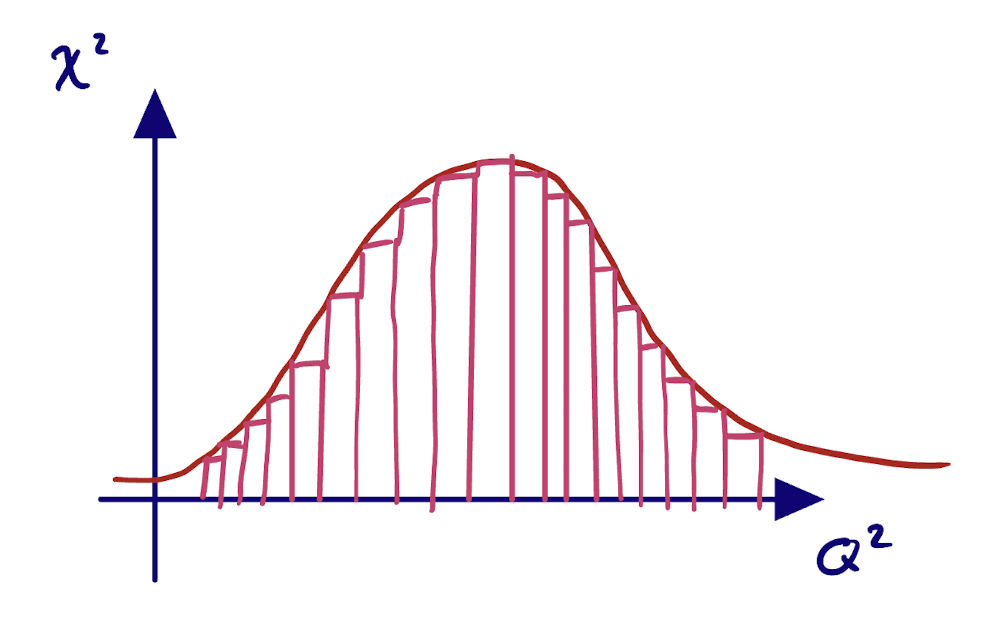
\includegraphics[scale = 0.36]{alpha}	

\end{wrapfigure}

\noindent Il fattore di scala cos\`{i} determinato non costituisce la sovrastima "reale" di cui si sono sbagliate le misure, poich\`{e} $\hat{Q^2}_{min}(\underline{x},\underline{\hat{\theta}}_{MQ})$ per $\underline{\hat{\theta}}_{MQ}$ fissato \`{e} anch'esso una variabile aleatoria  che segue la distribuzione di $\chi^2(N-K)$ di conseguenza la (5.26) stima un solo valore rispetto al campione a disposizione, ma $\alpha^2$ \`{e} una variabile aleatoria che segue la medesima distribuzione di $\hat{Q^2}_{min}(\underline{x},\underline{\hat{\theta}}_{MQ})$ e dunque per determinarlo bisogna ricostruire la distribuzione del $\chi^2$.

\section{Teorema di Gauss-Markov}
Si consideri un insieme di variabili aleatorie statisticamente indipendenti $\{(x_i,y_i)\}_i^N$ tali che sono legate tra loro da una relazione lineare rispetto ai parametri $y_i = \psi(x_i ,\underline{\theta}) + \epsilon_i$ dove $E[\epsilon_i] = 0$ e $V[\epsilon_i] $ finita $\forall i$ (propriet\`{a} di \textbf{omoschedasticit\`{a}}) ed inoltre $y_i$ indipendenti dai parametri $\underline{\theta} \Rightarrow$ si ha che lo stimatore $\underline{\hat{\theta}}$ ottenuto con il metodo dei minimi quadrati \`{e} non distorto e ha varianza minima fra tutti gli stimatori lineari.

\subsubsection{Osservazioni}

\begin{itemize}
	\item $\epsilon_{i}$ non \`{e} necessario che siano distribuite secondo una Gaussiana
	\item il teorema non ci dice che si \`{e} trovato lo stimatore pi\`{u} \textbf{efficiente} fra tutti gli stimatori possibili, ma sicuramente quello pi`{u} efficiente tra quelli lineari.
\end{itemize}  
\`{E} possibile trovare uno stimatore pi\`{u} efficiente per i parametri $\underline{\theta}$ per\`{o} dovremmo determinarlo con una funzione non lineare e ammesso che questa esista non \`{e} garantito che lo stimatore ottenuto sia non distorto.\newline
Gli stimatori descritti dal teorema di Gauss-Markov vengono definiti \textbf{B.L.U.E ( Best Linear Unbiased Estimator)}. 

\section{Interpolazione ed Estrapolazione}

\begin{wrapfigure}{l}{0.\textwidth}
\centering
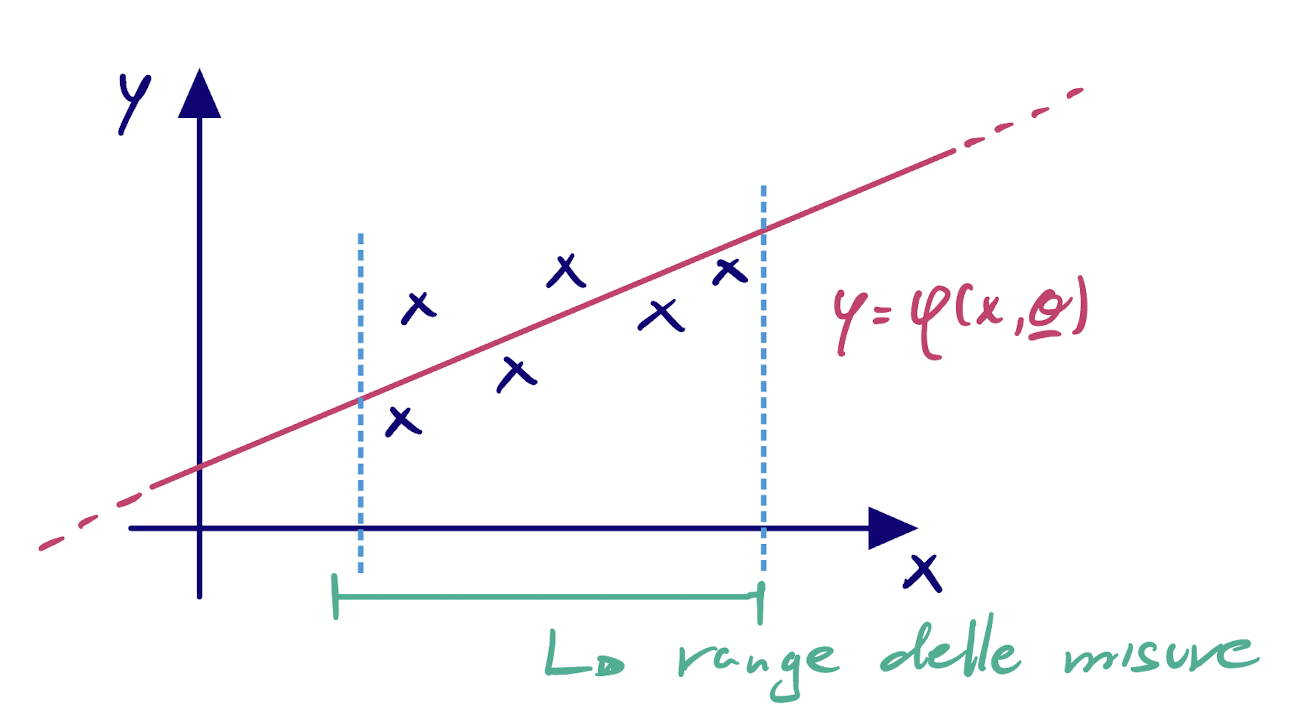
\includegraphics[scale = 0.35]{Estrapolazione}	
\end{wrapfigure}
Assumendo che i parametri $\underline{\theta}$ siano gi\`{a} stati determinati. \textbf{L'interpolazione} \`{e} la determinazione del valore di y mediante la funzione $\psi(x,\underline{\theta})$ per una misura x contenuta all'interno del range delle misure, ovvero l'intervallo contente i dati del campione. Si definisce \textbf{estrapolazione} il valore di y per qualsiasi altro valore di x non compreso all'interno del range delle misure definito sperimentalmente. Per una valore ottenuto da una retta di regressione lineare, l'errore \`{e} legato all'incertezza nella stima dei parametri di $\underline{\theta}$. Di conseguenza:

\begin{equation}
	V[y]_{i} = \nabla \psi(x,\underline{\theta})^T \cdot Cov[\underline{\hat{\theta}}_{MQ}] \cdot \nabla \psi(x,\underline{\theta}) 
\end{equation} 
Per esempio in un caso a due parametri si avr\`{a}:
\begin{align*}
V[y]_{i} = 
	\begin{bmatrix}
		\dfrac{\partial \psi}{\partial \theta_{1}} & & \dfrac{\partial \psi}{\partial \theta_{2}}  \\ 
	\end{bmatrix}
	\cdot 
	\begin{bmatrix}
		\sigma_{\theta_{1}}^2 & Cov(\theta_1,\theta_2) \\
		\\ 
		Cov(\theta_2,\theta_1) & \sigma_{\theta_{2}}^2 \\
	\end{bmatrix}
	\cdot 
	\begin{bmatrix}
		\dfrac{\partial \psi}{\partial \theta_{1}} \\
		\\
		\dfrac{\partial \psi}{\partial \theta_{2}} \\
	\end{bmatrix}
\end{align*}
che coincide con la formula di propagazione degli errori presente al capitolo 3. In generale l'errore aumenta allontanandosi dalla regione di campionamento ( quindi quando si passa dall'interpolazione all'estrapolazione).

\subsubsection{Esempio di fit lineare}

Consideriamo di avere un set di misure $\{(x_i,y_i) \}_{i}^N$ IID con incertezza $\sigma_{y_{i}}$ sulla variabile aleatoria y, e che il modello \`{e} quello di una retta y = a+bx, stimiamo i parametri a e b usando il metodo dei minimi quadrati. Avremo che:
\begin{align*}
\vec{\theta} =
	\begin{bmatrix}
		a \\
		b \\ 
	\end{bmatrix}
	\quad \quad \quad\vec{h}=
	\begin{bmatrix}
		1 \\
		x \\
	\end{bmatrix}
\end{align*}
e poich\`{e} le misure sono indipendenti tra loro, la matrice di covarianza \`{e} diagonale. Applicando il metodo dei MQ si stimano:
\begin{equation*}
	\hat{a} = \dfrac{1}{\sum_{i=1}^n \frac{1}{\sigma_i^2}}\sum_{i=1}^N \dfrac{y_i -\hat{b}x_i}{\sigma_i^2} = \overline{y} - \hat{b} \overline{x}
\end{equation*}

\begin{equation*}
	\hat{b} = \dfrac{1}{\sum_{i=1}^N \big (\frac{x_i}{\sigma_i} \big )^2}\sum_{i=1}^N \dfrac{y_ix_i -\hat{a}x_i}{\sigma_i^2} = \dfrac{\overline xy -\overline{x}\overline{y}}{\overline{x^2} - \overline{x}^2}
\end{equation*}
\newline
e le incertezze associate alle stime sono date dalla matrice di covarianza associate ai parametri:

\begin{align*}
V[\underline{\hat{\theta}}]=
	\begin{bmatrix}
		\sigma^2_{a} & Cov[a,b] \\
		Cov[b,a] & \sigma^2_{b} \\
	\end{bmatrix}
	= \textcolor{cyan}{\dfrac{\sigma^2}{N(\overline{x^2} - \overline{x}^2 )}} \cdot 
	\begin{bmatrix}
		\overline{x^2} & - \overline{x} \\
		- \overline{x} & 1 \\
	\end{bmatrix}
\end{align*} 

I termini in $\colorbox{cyan}{\phantom{b = \,}}$ viene definito \textbf{dispersione delle misure}. Si osserva che non necessariamente i parametri sono scorrelati tra loro. Pi\`{u} le msiure sono sparpagliate meigliore \`{e} la precisione con cui si stimano i parametri, poich\`{e} la banda che definisce le possibili rette che fittano i dati diventa pi\`{u} sottile, inoltre anche il numero di misure fornisce un contributo alla precisione con cui si determinano gli stimatori. \newline

\noindent Se calcoliamo il valore assunto dalla funzione in punto $x_0$ rispetto ai parametri $\hat{a}$ e $\hat{b}$ si ricava che l'errore su $y_0$ \`{e} dato da:

\begin{equation*}
	V[y_0] = \dfrac{\sigma^2}{N} \Big[ 1 + \dfrac{(x_0 - \overline{x})^2}{(\overline{x^2} - \overline{x}^2 )^2} \Big ]
\end{equation*}
Pi\`{u} $x_0$ si allontana da $\overline{x}$ pi\`{u} \`{e} grande la varianza su $y_0$.

\section{Fit d'istogrammi}

\begin{wrapfigure}{l}{0.\textwidth}
\centering
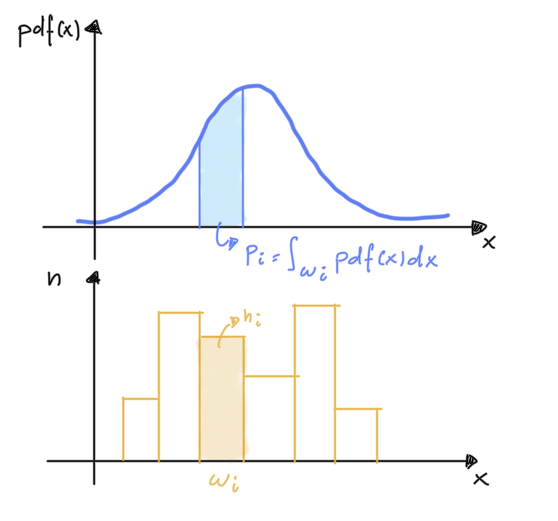
\includegraphics[scale = 0.34]{BinnedData}	
\end{wrapfigure}
Consideriamo un insieme di N misure $\{x_{i}\}_i^N$ IID che seguono la pdf $f(x_i,\vec{\theta}): \Omega \subseteq \mathbb{R} \rightarrow \mathbb{R}$, raccogliamo i dati in modo da dividere l'asse reale in k intervalli $\omega_j = [x_i,x_{i+1})$. tali che $\omega_j \cap \omega_i = \varnothing \quad \forall i,j$ e $\bigcup_{j=1}^k \omega_j = \Omega$. Tali intervalli vengono defini 'bin', per ciascuno di essi contiamo il numero di misure $n_j$ che cadono all'interno dell'intervallo. Complessivamente avremo che $\sum_{j=1}^N n_j = N$ numero totale di misure. Poich\`{e} le misure sono IID a ciascuna bin associamo una probabilit\`{a}:
\begin{equation*}
	p_j = \int_{\omega_j}pdf(x,\vec{\theta})dx \quad \forall j =1,...k
\end{equation*} 

\begin{wrapfigure}{r}{0.\textwidth}
\centering
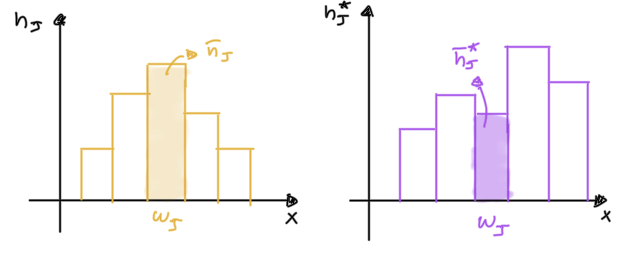
\includegraphics[scale = 0.32]{expbin}	
\end{wrapfigure}
\noindent Partendo dalla probabilit\`{a} associata a ciascun bin $\omega_j$ costruiamo un istogramma i cui conteggi attesi sono dati da i $ E[n_{j}] = N \cdot p_j(\vec{\theta})$. Le misure di conteggio dell'istogramma definito dai dati del campione seguono una joint-pdf $pdf(n_1,...,n_k,p_1,...p_k)$ che definisce una distribuzione multinomiale. Per $p \rightarrow 0 $ le misure di conteggio sono statisticamente indipendenti tra loro di conseguenza la multinomiale pu\`{o} essere riscritta come prodotto di distribuzioni di probabilit\`{a} binomiali.
\begin{equation*}
	pdf(n_1,...,n_k,p_1,...,p_k) = \prod_{i=1}^kpdf(n_i,p_i)
\end{equation*}
Nel caso in cui il valore di aspettano del conteggio dei bin sia costante possiamo approssimare le singole pdf binomiali come delle Poissoniane dove $\lambda_{i}(\vec{\theta}) = N * p_i(\vec{\theta})$ rappresenta la frequenza media di eventi della distribuzione di Poisson di conseguenza la joint-pdf diventa :
\begin{equation*}
	\prod_{i=1}^kpdf(n_i,p_i) = \prod_{i=1}^k \dfrac{\lambda_i(\vec{\theta})^{n_{i}}}{n_{i}!}e^{-\lambda_{i}} = L(n_1,...,n_k,\theta)
\end{equation*}
Che coincide con la extended likelihood.\newline
Non solo si conosce la pdf associata ai dati ma anche il loro valore di aspettazione e varianza di conseguenza \`{e} possibile applicare il metodo di ML e dei MQ.

\subsubsection{Osservazioni}

Utilizzare le misure binnate ci permette di ridurre le dimensioni dei dati con cui si lavora, anche se si ha una perdita d'informazione questa viene bilanciata da una maggiore semplicit\`{a} e dalla possibilit\`{a} di usare differenti tecniche per la stima dei parametri, come per esempio quella di ML che per campioni molto grandi risulta essere da un punto di vista computazionale dispendiosa.

\subsection{Binned Data - Minimi Quadrati}

Applichiamo il metodo dei minimi quadrati confrontando i conteggi dell'istogramma dei dati con l'istogramma dei valori attesi. Dato un campione $\{x_i\}_i^N$ IID dopo averli rappresentati in un istogramma, associamo al valore atteso di conteggi per ciascun bin l'espressione:
\begin{equation*}
	\mu_i = E[n_j] = N \cdot \int_{\omega_j}pdf(x, \vec{\theta})dx = N \cdot p_j(\vec{\theta}) 
\end{equation*}
Scrivendo il funzionale $Q^2$ come:
\begin{equation*}
Q^2 = \sum_{i=1}^N\dfrac{(n_i - E[n_i])^2)}{V[n_i]}	 = \sum_{i=1}^N\dfrac{(n_i - Np_i(\vec{\theta}))^2)}{Np_i(\vec{\theta})} 
\end{equation*}
Assumendo che i conteggi $n_i$ seguano una pdf Poiss$(n_i,\mu_i)$ (la discussione che segue risulterebbe verificata ugualmente anche se le pdf fossero binomiali). Per $n_i \rightarrow \infty$ possiamo approssimare la poissoniana a una gaussiana con valore atteso e varianza pari a $\mu_i$ di conseguenza $Q^2$ dipendendo da variabili aleatorie distribuite secondo una gaussiana, ed essendo lui stesso una variabile casuale si ha che segue la distribuzioni di $\chi^2(k-s)$ dove s \`{e} il numero di parametri. Definiamo dunque il $\chi^2$ nella forma di \textbf{Neyman}:
\begin{equation}
	\chi^2_{Neyman} = \sum_{i=1}^N\dfrac{(n_i - \mu_i(\vec{\theta})^2)}{n_i} = \sum_{i=1}^N\dfrac{(O_i - E_i)^2}{O_i}
\end{equation} 
Dove per $n_i$ grande si \`{e} approssima $V[n_i] \approx n_i$. La necessit\`{a} di approssimare i dati a una Gaussiana e la varianza al numero di conteggi di un bin, \`{e} determinata dal fatto che cos\`{i} facendo il teorema di Gauss-Markov risulta soddisfatto poich\`{e} tra le ipotesi \`{e} necessario che i momenti non dipendano dai parametri. In conclusione di procede a minimizzare il $\chi^2_{Neyman}$ per determinare i parametri $\vec{\theta}$.

\subsubsection{Procedura di fit di un istogramma}
La procedura di fit di un istogramma con il metodo del $\chi^2$ di Neyman prevede quindi di:

\begin{itemize}
	\item verificare che sia rispetta l'ipotesi pdf($n_i$) gaussiana;
	\item associare a $n_i$ un errore $\sqrt{n_i}$
	\item calcolare per ogni valore del parametro $\theta_i$ i valori attesi $\mu_i$ dei conteggi in ciascun bin;
	\item minimizzare il $\chi^2_{Neyman}$ trovando il valore di $\theta$ per cui l'accordo valori misurati - valori attesi \`{e} il migliore;
	\item all'occorrenza effettuare un test del $\chi^2$
	\end{itemize}
	
	\subsection{Binned Data - Maximum Likelihood}
	Fare il fit di un'istogramma quando non vale l'approssimazione Gaussiana prevede necessariamente l'utilizzo della binned Maximum Likelihood. Analogamente a quanto discusso a inizio sezione si procede a passare discretizzare il modello. Dove la funzione di likelihood associata al campione \`{e} data da
	
	\begin{equation*}
		L(n_1,...,n_k,\vec{\theta}) = \prod_{i}^k Bin(n_i,p_i(\vec{\theta},N)
	\end{equation*}
e si procede a massimizzare la funzione di likelihood:
\begin{equation*}
	\dfrac{\partial L(\vec{n},\vec{\theta})}{\partial \theta_j}= 0 \quad \quad \forall j=1,...,k
\end{equation*}
Ad un bin-size deve essere associata una probabilit\`{a} $p_{i}(\vec{\theta})$ piccola. Non \`{e} necessario che i bin abbiano tutti la stessa dimensione, possiamo sceglierle in modo che $N \cdot p_i$ sia grande e quindi valga l'approssimazione Gaussiana.\newline

L'operazione di binning, fa perdere informazione, questo si pu\`{o} riflettere sull'incertezza del parametro stimato , ma anche sulla capacit\`{a} di verificare che i dati siano ben descritti dal modello. In questi casi \`{e} utili studiare la dipendenza del risultato dal binning.




\setcounter{chapter}{5}
\chapter{Test d'ipotesi}

\section{Test del $\chi^2$}

Consideriamo un campione di N misure $\{(x_i,y_i)\}_i^N$ IID legate tra loro da una funzione $y =\psi(x,\vec{\theta})$ avremo che le misure campionate rispetto alla variabile aleatoria y, possono essere riscritte come $y_i = \psi(x,\vec{\theta}) + \epsilon_i$ dove $\epsilon$ ipotizziamo essere una variabile aleatoria la cui $pdf(\epsilon)$ segue una distribuzione di probabilit\`{a} Gaussiana. Nell'ipotesi in cui valga il TCL per le $\epsilon_i$, si ha che il $Q^2$ associato alle misure e il modello segue la distribuzione di $\chi^2(N-k)$.

 
\begin{figure}[ht]
\vspace{0.2in}
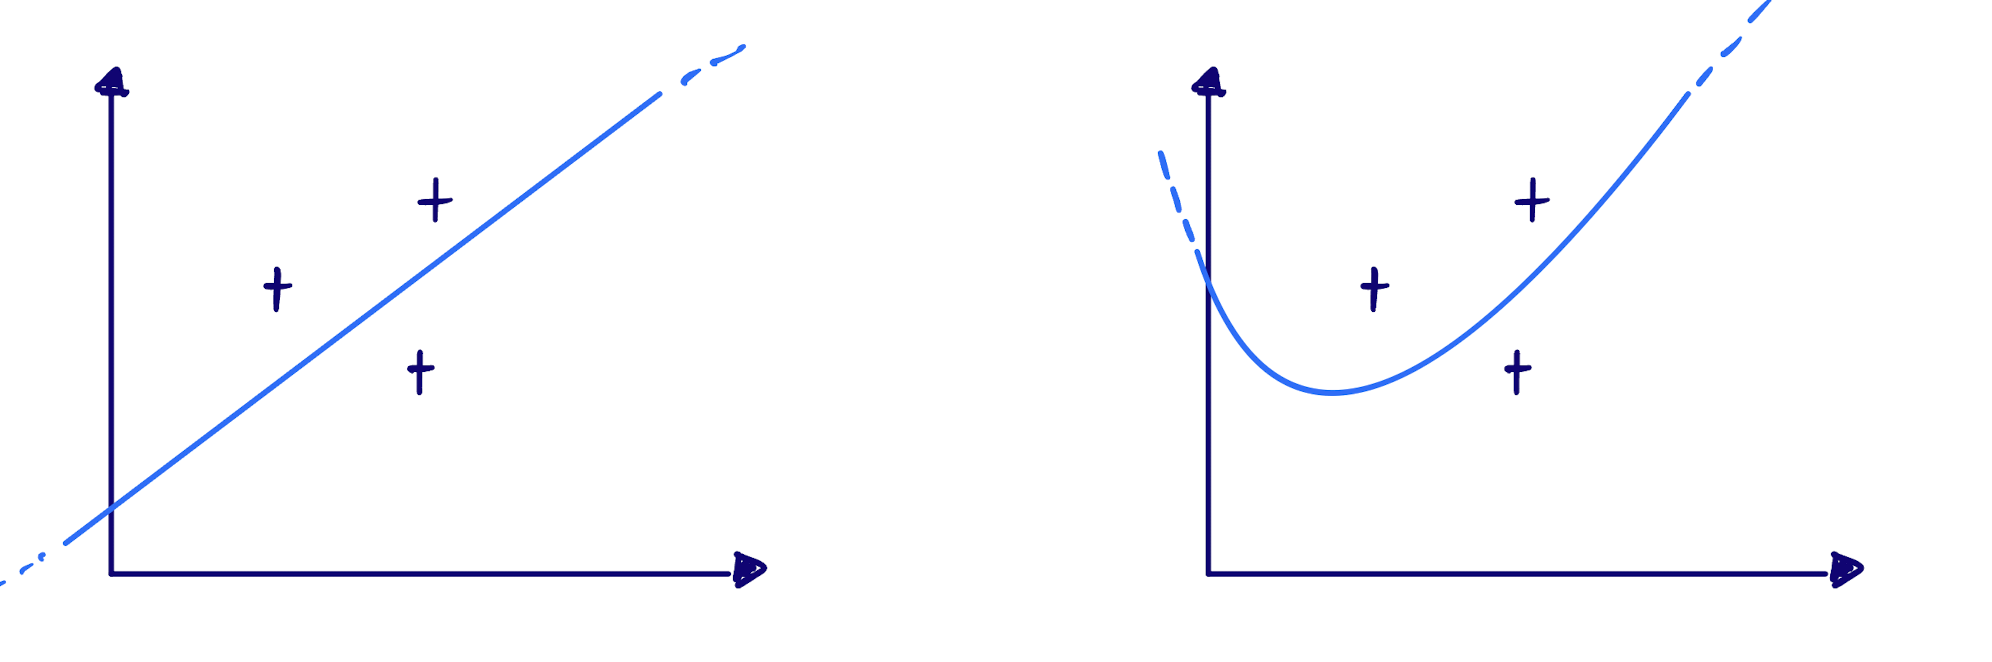
\includegraphics[scale = 0.35]{compa}	
\centering
\vspace{0.1in}
\caption{Due modelli differenti che interpolano lo stesso campione di dati.}
\end{figure} 
\noindent Nel caso di destra in figura 6.1 gli scarti quadratici sono minori, mentre in quello di destra sono pi\`{u} grandi, di conseguenza possiamo aspettarci che il valore di aspettazione della distribuzione di $\chi^2$ del modello di sinistra sia pi\`{u} grande di quello di destra. Definiamo il modello non corretto (quello di sinistra) $H_1$ e il modello corretto (quello di destra) $H_0$, la domanda che possiamo porci \`{e}: " Se partiamo da due ipotesi $H_1$ e $H_0$ e non sappiamo quale delle due sia corretta, come facciamo a determinare quella che descrive meglio la realt\`{a} sperimentale? ". \newline
Introduciamo una nuova quantit\`{a} definita \textbf{p-value} che ha la seguente espressione :
\vspace{0.2in}

\begin{minipage}{.4\textwidth}
	\begin{equation}
		\text{p-value} = \int_{\overline{Q}^2}^{\infty}\chi^2(N-k)d\chi^2 
	\end{equation}
  \end{minipage}
  \begin{minipage}{.4\textwidth}
    \centering
    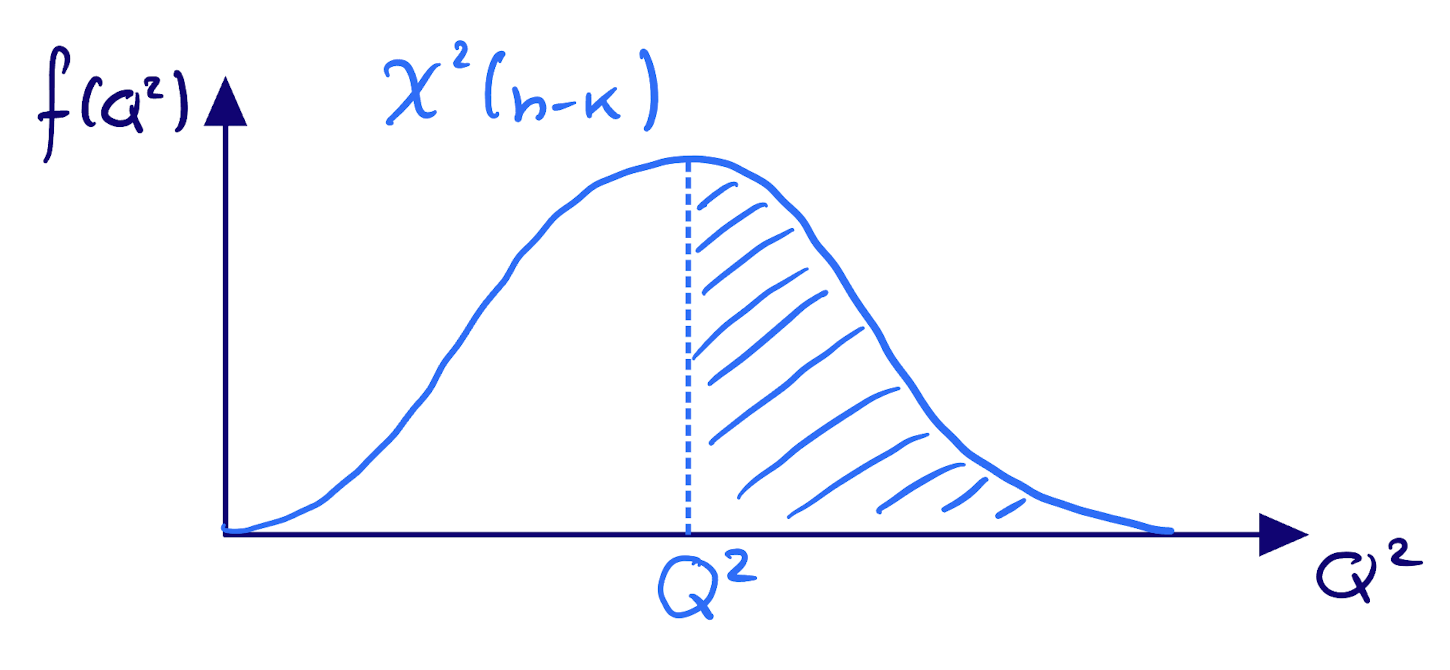
\includegraphics[scale = 0.3]{pvalue}	
  \end{minipage}
\vspace{0.2in}

\noindent la quantit\`{a} cos\`{i} definita risulta essere una misura di probabilit\`{a}. Per rispondere alla domanda precedente fissiamo una soglia di tolleranza del p-value oltre alla quale i valori ottenuti risultano essere dei \textbf{falsi negativi}. Riprendendo i modelli $H_0$ e $H_1$ che definiamo rispettivamente \textbf{null hypothesis} e \textbf{alternative hypothesis}, fissata una soglia del p-value, e definita una statistica x associata (come per esempio il $Q^2$) al $\chi^2(x \vert N-k)$ avremo che:
\begin{itemize}
	\item H0 \`{e} rigettata se x cade nella regione in azzurro $\omega_\alpha^* $ in figura 6.2
	\item H0 \`{e} accettata se x cade nella regione in verde $\omega_\alpha$ nella figura sottostante.
\end{itemize}
\begin{figure}[ht]
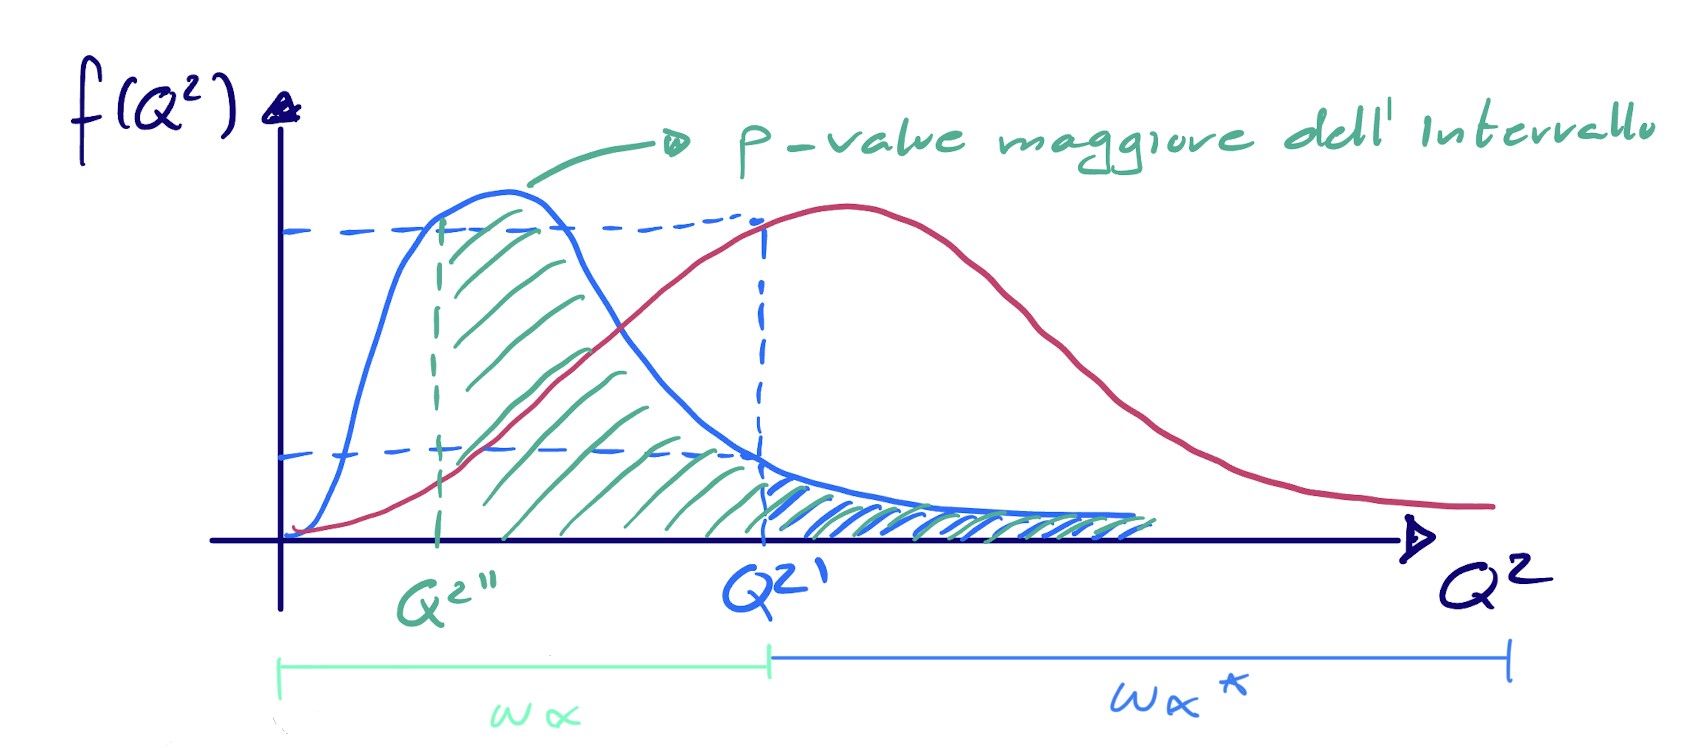
\includegraphics[scale = 0.4]{hypo}	
\centering
\end{figure}
Dunque date due ipotesi $H_0$ e $H_1$ decidiamo di considerare affermativa quella che restituisce il valore del p-value pi\'{u} alto (ovvero quella con probabilit\'{a} maggiore) rispetto al valore $p_0$ di soglia considerato, apparentemente sembrerebbe sufficiente per concludere quale delle due ipotesi sia verifica, ma in realt\'{a} come si vedr\'{a} nelle sezioni succesive la realt\'{a} sperimentale \'{e} pi\'{u} complicata e posso esserci casi di falso positivi.

\noindent Su quanto discusso fino ad ora possiamo fare le seguenti osservazioni:
\begin{itemize}
	\item I minimi quadrati permettono di calcolare il $Q^2$ (e anche il metodo di ML calcola i parametri $\hat{\theta}$ da cui si può calcolare il $Q^2$);
	\item Il test del $\chi^2$ \'{e} applicabile se sappiamo calcolare il valore del $Q^2 \Rightarrow \sigma^2$  deve essere nota e ben stimata;
	\item Test del $\chi^2$ \`{e} un test integrale $\Rightarrow$ Somma gli scarti su tutti gli eventi, e dunque pu\'{o} presentare delle limitazioni (esempio sotto).
\end{itemize}

\subsubsection{Esempio}

\begin{wrapfigure}[18]{l}{0.\textwidth}
\centering
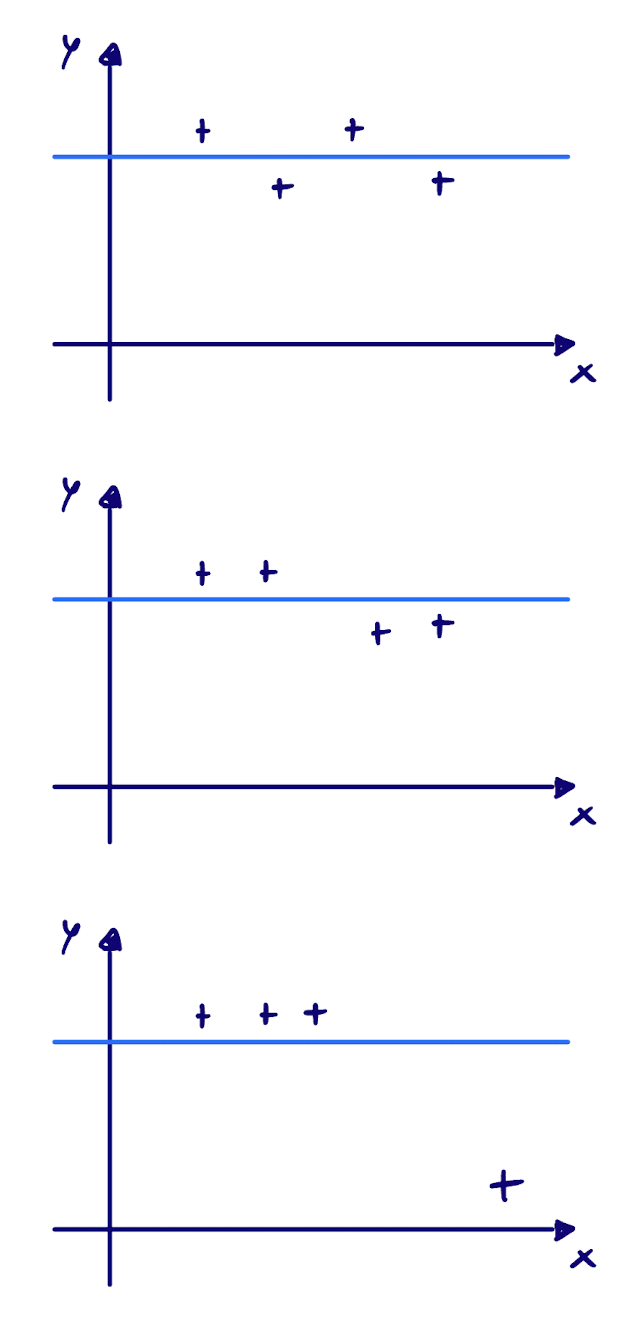
\includegraphics[scale = 0.5]{esempio}	
\end{wrapfigure}

Assumiamo che il p-value sia accettabile ovvero maggiore
dell'intervallo di confidenza. Consideriamo gli stessi punti 
riorganizzati in un modo diverso, ma con stesso scarto quadratico.
I due set di dati con y differenti hanno lo stesso p-value.

Essendo che il test del $\chi^2$ ha una forma integrale, se
graficamente si osserva una distribuzione differente delle
misure, il test non lo tiene in considerazione.

Se consideriamo una dispersione delle misure come nella terza figura e
assumiamo che abbia il medesimo p-value delle altre due, si ha
che il test non considera che i dati diminuiscono di valore lungo l'asse delle ordinate e dunque si ottiene un \textbf{falso positivo}, ovvero p-value \`{e} verificato, ma il modello non descrive adeguatamente il comportamento dei dati sperimentali.
Il fatto che il test del $\chi^2$ abbia forma integrale limita la generalit\`{a} con cui possiamo decidere se il risultato ottenuto sia affidabile o meno.
\newline
\newline
\textbf{Definizione di Overfitting}

\begin{wrapfigure}{r}{0.\textwidth}
\centering
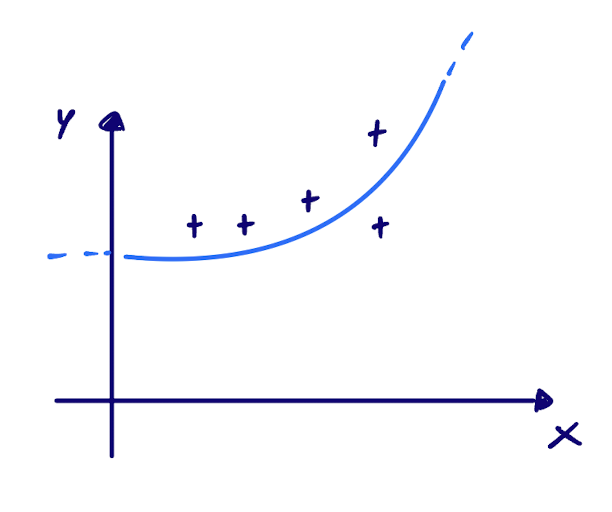
\includegraphics[scale = 0.5]{overfit}	
\end{wrapfigure}
\vspace{0.05in}

\noindent Ipotizziamo di avere un fit che ha $Q^2$ = 0 e p-value-1,
ovvero i dati vengono interpolati perfettamente , questo non \`{e}
un buon risultato. Si ha un caso di overfitting, dove si sono introdotti così tanti parametri che
il risultato del fit si \`{e} completamente adattato alle misure, perdendo qualsiasi
capacit\`{a} di generalizzare il modello. 

\subsection{Applicazione del test di $\chi^2$}

Se il modello \`{e} corretto $y = \psi(x,\vec{\theta})$, allora il metodo dei MQ fornisce una stima dei parametri $\vec{\theta}$ che lo descrivono. Il valore stimato dei parametri rappresenta il punto di minimo del funzione di $Q^2_{min} = Q^2(x,\vec{\theta}_{MQ})$ rispetto al campione sperimentale, tale punto di minimo coincide anche con il massimo della distribuzione di $\chi^2$ se pdf($\epsilon$) seguono una distribuzione gaussiana, che \`{e} dato da $E[Q^2] = N-k$ e quindi $Q^2_{min} = N-k$. \newline
Il $\chi^2$ ridotto \`{e} definito come $\chi^2_{0} = \frac{\chi^2}{N-k}$ ci\`{o} implica che per $\chi^2 = Q^2_{min}$ il ridotto \`{e} $\chi^2_0 \sim 1$. \newline
Se il valore del $\chi^2$ \`{e} lontano dal suo valore di aspettazione N-k (o 1 nel caso si usi quello ridotto), possiamo concludere che alcune delle ipotesi precedenti non sia corrette e dunque \textbf{i dati non confermano il modello}. 

\noindent Le regioni a bassi valori di $\chi^2$ corrispondono a scarti tra modello e dati molto piccoli, quindi a casi di overfitting. Tali risultati sono altamente improbabili e possono essere dovuti a sovrastime degli errori, la loro pdf non \'{e} Gaussiana o se le incertezze considerate non sono solo di natura sistematica. 

\begin{figure}[ht]
\vspace{0.1in}
\includegraphics[scale =0.4]{testchi}	
\centering
\caption{Overfitting}
\end{figure}

\subsection{Distribuzione di probabilit\'{a} del p-value}
Poich\'{e} $Q^2$ \'{e} una variabile aleatoria anche il p-value lo \'{e} e dunque possiede una sua distribuzione di probabilit\'{a}, per determinarla consideriamo un cambio di variabili:
\begin{equation*}
	x: f(x) \text { se } u^{-1}(y)=v(y) \quad \Rightarrow \quad y: a(x) \rightarrow g(y)=f(v(y)) \cdot\left|v'(y)\right|
\end{equation*}
Posto $x = Q^2$, $y=p$ e f = $\chi^2$ si ha che :
\begin{equation*}
	u(x) \rightarrow 1-X \quad X(x)=\int_{-\infty}^{x} \chi^2(t, n) d t \quad e \quad v(y)=(1-X)^{-1}
\end{equation*}
e quindi:
\begin{equation*}
	g(y)=\chi^2\left(Q^2\right)\left|\frac{1}{(1-X)^{\prime}\left(Q^2\right)}\right|=\frac{\chi^2\left(Q^2\right)}{\chi^2\left(Q^2\right)}=1
\end{equation*}
\newline
\noindent di conseguenza  il p-value segue una \textbf{distribuzione uniforme}. 
\newline

\noindent Un test che \'{e} possibile fare per verificare se le condizioni iniziali affinch\'{e} il test del $\chi^2$ sia applicabile \'{e} quello di verificare che ripetendo le misure il p-value segua una distribuzione uniforme.
\section{Errori di test statistici}

Quanto discusso in questa sezione fa riferimento al test del $\chi^2$, ma generalizzabile a qualsiasi statistica $\beta$ per cui \'{e} possibile definire due distribzioni di probabilit\'{a}:

\begin{itemize}
	\item $pdf(\beta \vert H_0)$ = \textbf{Null Hypothesis 
	\item $pdf(\beta \vert H_1)$ = \textbf{Alternative Hyp}othesis}
\end{itemize}
\subsection{Errori del $I^{\circ}$ tipo}

Un errore del primo tipo rappresenta il numero di casi veri per la null hypothesis Ho che scartiamo fissata una soglia del p-value.

\vspace{0.3in}
\begin{minipage}{.4\textwidth}
	\begin{equation}
		\alpha = \int_{\overline{Q}^2}^{\infty}\chi^2(N-k)d\chi^2 
	\end{equation}
  \end{minipage}
  \begin{minipage}{.4\textwidth}
    \centering
    \includegraphics[scale = 0.4]{size}	
  \end{minipage}
\vspace{0.2in}

Il termine $\alpha $ prende il nome di \textbf{size del test}. 

\subsection{Errori del $II^{\circ}$ tipo}

 Un errore del secondo tipo rappresenta la probabilit\`{a} di accettare H0 quando \`{e} vera H1, in questo caso si parla di \textbf{falsi positivi}. 
 \vspace{0.2in}
 
\begin{minipage}{.4\textwidth}
	\begin{equation}
		\beta = \int_{Q^2}^{\overline{Q}^2}\chi^2(N-k)d\chi^2 
	\end{equation}
  \end{minipage}
  \begin{minipage}{.4\textwidth}
    \centering
    \includegraphics[scale = 0.3]{powertest}	
  \end{minipage}
\vspace{0.2in}

Si sta commettendo un errore poich\`{e} se H1 \`{e} la forma funzionale sbagliata il fit dei dati supera ugualmente il test del $\chi^2$. 

\noindent Il termine $1-\beta$ prendere il nome di \textbf{power del test} e restituisce la probabilit\`{a} di rifiutare $H_0$ quando $H_1$ \`{e} vera.
\newline

\noindent Fissate le due ipotesi alternative e definiti gli intervalli di confidenza, se si assume che l'errore di tipo uno sia quello pi\`{u} grave si procede scegliendo la percentuale di falsi negativi che si reputa accettabile e si cerca di definire gli intervalli $\omega_\alpha$ e $\omega_\alpha^*$ in modo tale che $\beta$ sia il minore possibile (minor caso di falsi positivi). Il test cos\`{i} descritto viene definito il pi\`{u} potente per un determinato valore di soglia del p-value.

\section{Test di Kolgomorov-Smirnov}

Consideriamo un insieme di N misure della stessa grandezza fisica X vogliamo testare la null hypothesis $H_0$ che siano campionamenti di una determinata pdf che prendiamo come riferimento. Una possibilit\`{a} \`{e} di usare il test del $\chi^2$ applicandolo agli istogrammi costruiti con le misure raccolte e la pdf-modello. Tale procedura \`{e} corretta, ma richiedere di binnare i dati e dunque si ha una perdita d'informazione, inoltre l'esito del test pu\`{o} dipendere dal binning scelto per la costruzione degli istogrammi.

L'alternativa \`{e} data dal test di \textbf{Kolgomorv-Smirnof} che confronta le due distribuzioni cumulative (dati - pdf-modello) e in questo modo sfrutta tuta l'informazione contenuta nei dati. Tale test \`{e} di tipo non parametrico ovvero non richiede la costruzione di stimatori rispetto ai dati raccolti sperimentalmente e viene utilizzato per variabili aleatorie continue. 


\subsection{Costruzione del test}

Date N misure ordinate in senso crescente, ricostruiamo la distribuzione cumulativa della pdf-modello, definendo una funzione a gradini $S_n (x)$ rispetto ai dati del campione, tale funzione prende il nome di \textbf{EDF (Empirical Distribution Function)}, la scelta ricade su una funzione di questo tipo poich\`{e} sono presenti dei buchi nell'informazione (campione) raccolta. La forma dell'EDF \`{e} data:

\begin{equation}
	S_n(x) = \sum_{i=1}^nI(x_i \leq x)  
\end{equation}
dove la funzione $I(x_i \leq x)$ prende il nome di \textbf{indicator function} ed \'{e} espressa come:

\vspace{0.2in}

\begin{minipage}{.4\textwidth}
	\begin{align*}
I(x) = 
	\begin{cases}
	1 \quad x \leq x_{i+1} \\
	0 \quad \quad \quad \text{altrimenti}\\
	\end{cases}
\end{align*}
  \end{minipage}
  \begin{minipage}{.4\textwidth}
    \centering
    \includegraphics[scale = 0.3]{step}	
  \end{minipage}
\vspace{0.2in}

Ci si domanda quanto bene $S_n$ approssimi la cumulativa F(x), la risposta \`{e} che dipende dal numero di misure contate prima del gradino successivo e quindi da come si scelgono gli intervalli. Per valutare l'approssimazione per ogni punto distinto che costituisce un estremante degli intervalli $\tilde{x}$ valutiamo l'estremo superiore della differenza tra la EDF e la pdf con cui vogliamo confrontarla:
\begin{equation*}
	D_n = \sup_{x} \vert S_n(x) -F(x) \vert 
\end{equation*}
 la distanza $d_n \equiv \sqrt{n}D_n$ definisce il valore di riferimento per il test di KS che consiste nel confrontare tale numero con una grandezza di riferimento $d_0$, che costituisce la quantit\'{a} di soglia rispetto alla quale rigettare la null hypothesis $H_0$. Se $d > d_0$ l'ipotesi di compatibilit\`{a} viene rigettata. Il valore di $d_0$ \`{e} scelto in base alla probabilit\`{a} che la variabile casuale $d$ sia maggiore di $d_0$ quando il modello \`{e} corretto.
 \begin{equation*}
 	P( d > d_0 \vert H_0) = \alpha
 \end{equation*}
Tale metodo non parametrico \`{e} anche utile per confrontare due campioni di dati al fine di determinare se provengono dalla stessa popolazione. Si noti anche che la \textbf{EDF(x)} costruita \`{e} anch'essa una distribuzione cumulativa di probabilit\'{a}.
 
 \section{Confronto di una misura con il valore di riferimento}
 
 \subsection{Distribuzione t-student}
 Si consideri un campione di N misure di cui si \`{e} calcolata la media campionaria $\overline{x} = \frac{1}{N} \sum x_i$ e si supponga di conoscere $\sigma_i$ delle singole misure e $E[x] = \mu$, allora la media aritmetica $\overline{x}$ \`{e} per il TCL \`{e} distribuita come una gaussian G($\overline{x}$,$\mu$, $\frac{\sigma}{\sqrt{N}}$). Come facciamo a dire che $\overline{x}$ e ${\mu}$ sono sufficientemente vicine tra loro rispetto alle incertezze ?
 \newline
 Per determinare la distanza tra le grandezze definiamo la distribuzione t-student data dalla variabile aleatoria:
 
 \begin{equation*}
 	t = \dfrac{\vert \overline{x} - \mu\vert }{\frac{\sigma}{\sqrt{N}}}
 \end{equation*}
 definita rispetto al caso descritto nelle righe precedenti. In generale la t-student per un parametro \`{e} data da:
 \begin{equation}
 	t = \dfrac{\vert \hat{\theta}^* - \theta_t \vert}{\sigma_{\theta^*}}
 \end{equation}
 
 Notare che nel caso in cui si conoscano a priori l'incertezza della misura che si sta confrontando, dunque non si \`{e} ottenuta mediante un processo statistico si ha che la pdf(t) \'{e} Gaussiana.
 Se $\overline{x}$ segue una pdf Gaussiana e $Q^2 \sim \chi^2(N-1)$ la distibuzione di t-student ha la seguente forma funzionale.
 
 \begin{equation}
 	f(t,\nu = N-1) = \dfrac{1}{\sqrt{n\nu}} \cdot \dfrac{\Gamma({\frac{\nu+1}{2}})}{\Gamma(\frac{\nu}{2})} \cdot \Big (1 + \frac{t^2}{\nu} \Big) ^{-(\frac{\nu+1}{2})}
 \end{equation}
 
 \subsubsection{Propriet\`{a} della distribuzione}
 \begin{align*}
 	\begin{matrix}
 		\mu = E[t] = 0 & \quad \quad & \gamma_1 = 0 \\
 		\\
 		\sigma^2 = V[t] = \frac{\nu}{\nu-2} \quad \nu > 2 & \quad \quad & \gamma_2 = \frac{6}{\nu-4} \quad \nu > 4
 	\end{matrix}	
 \end{align*}
 \newline
 Per $\nu = g.d.l. \rightarrow \infty$ la distribuzione diventa Gaussiana. Si osserva che la pdf della t-student \`{e} un po' pi\`{u} larga della distribuzione Gaussiana (fig 6.2).
 
  
\begin{figure}[ht]
\vspace{0.1in}
\includegraphics[scale = 0.4]{student}	
\centering
\vspace{0.1in}
\caption{Confronto distribuzioe di Gauss e t-student}
\end{figure}
In generale possiamo vedere la distribuzione della t-student come il rapporto tra una Gaussiana normalizzata e la radice di  $\frac{\chi^2}{N-1}$.
\begin{equation*}
	t = \dfrac{\vert \overline{x} - \mu \vert}{\Big [{\dfrac{\hat{\sigma}^2}{N}} \Big ]^{\frac{1}{2}}} = \textcolor{cyan}{\dfrac{\vert \overline{x} - \mu \vert}{\Big [{\dfrac{\sigma^2}{N}} \Big ]^{\frac{1}{2}}}} \cdot \textcolor{red}{\dfrac{\Big [ \dfrac{\sigma^2}{N} \Big]^{\frac{1}{2}}}{\Big [ \dfrac{\hat{\sigma}^2}{N} \Big]^{\frac{1}{2}}}} = \textcolor{cyan}{\dfrac{\vert \overline{x} - \mu \vert}{\Big [{\dfrac{\sigma^2}{N}} \Big ]^{\frac{1}{2}}}} \cdot \textcolor{red}{\Big [ \dfrac{\chi^2}{N-1} \Big ]^{\frac{1}{2}}}  
\end{equation*}
la parte in azzurro segue la pdf di una Gaussiana normalizzata N(0,1), mentre la parte in rosso segue $\frac{\chi^2}{N-1}$. Dove:
\begin{equation*}
	\textcolor{red}{\dfrac{1}{\Big [ \dfrac{\sigma^2}{\hat{\sigma}^2} \Big ]^{\frac{1}{2}}} = \dfrac{1}{\Big[  \frac{N-1}{\chi^2} \Big ]^{\frac{1}{2}} } = \Big [ \dfrac{\chi^2}{N-1} \Big ]^{\frac{1}{2}}  } 
\end{equation*}
\begin{wrapfigure}{r}{0.\textwidth}
\includegraphics[scale = 0.3]{Bellcurve}	
\centering
\end{wrapfigure}
Per la t-student fissato un valore di soglia $t_0$, ci permette di determinare la compatibilit\`{a} tra il valore stimato e quello atteso, se $t>t_0$ allora le due misure risultano essere non compatibili tra loro. Dove gli intervalli di compatibilit\`{a} risultano essere in multipli di deviazioni standard.

\subsubsection{Confronto tra la stima di due parametri}

La distribuzione di t-student pu\`{o} essere utilizzata non solo per confrontare una misura con un valore atteso, ma anche due stime del medesimo parametro tra loro.

\begin{equation}
	z = \dfrac{\vert \theta^*_1 - \theta^*_2 \vert }{ \Big [\dfrac{\hat{\sigma_1}}{N} +\dfrac{\hat{\sigma_2}}{N} \Big ]^{\frac{1}{2}}}
\end{equation}
dove la pdf(z) \`{e} Gaussiana se $\sigma_1$ e $\sigma_2$ sono senza errore, mentre altrimenti segue una distribuzione di t-student con N-M-2 gradi di libert\`{a}.

\section{Intervalli di confidenza}

Ipotizziamo che lo stimatore $\hat{\theta}$ segue una distribuzione gaussiana G($\hat{\theta},\theta_t,\sigma$) determinato il suo valore $\theta^*$ ci domandiamo quale sia la probabilit\`{a} che tale valore disti $\sigma$ dal valore vero $\theta_t$, ovvero $P[\theta^* \in (\theta_t - \sigma, \theta_t + \sigma)]$ = 0,68. Essendo $\theta^*$ una variabile aleatoria dipendente dal campione mentre $\theta_t$ no, l'affermazione precedente non \`{e} corretta, in quanto $\theta_t$ non \`{e} una variabile aleatoria, per questo motivo riscriviamo l'intervallo di confidenza in $ \theta_t \in (\theta^* - \sigma,\theta^* + \sigma)$ e la probabilit\`{a} come $P[\theta_t \in (\theta^* - \sigma, \theta^* + \sigma)]$ = 0,68, determinando un 68 \% di confidenza nell'intercettare $\theta_t$ ripetendo l'esperimento.
\begin{figure}[ht]
\vspace{0.1in}
\includegraphics[scale = 0.44]{intervaltheta}	
\centering
\end{figure}

\subsection{Metodo della cintura di confidenza}

Definiamo uno stimatore $\hat{\theta} \equiv \hat{\theta}(x)$, di un parametro $\theta$ rispetto ad un campione di N variabili aleatorie IID di una grandezza x, poich\`{e} lo stimatore dipende da variabili aleatorie anch'esso \`{e} una r.v. di conseguenza seguir\`{a} una distribuzione di probabilit\`{a} $f(\hat{\theta} \;\vert \; \theta)$. Per ciascun campione raccolto $\hat{\theta}$ definir\`{a} una stima $\theta^*$ del parametro, costruendo la pdf associata. Ripetendo l'esperimento con diversi campionamenti ciascuna distribuzione relativa  avr\`{a} un valore atteso $E[\hat{\theta}] = \theta_{t}^{i}$ e una varianza $V[\hat{\theta}] = \sigma_{\theta_{t}^i}^2$.
\begin{wrapfigure}{r}{0.\textwidth}
\centering
\includegraphics[scale = 0.4]{confidence}	
\end{wrapfigure}
Per ciascun esperimento non conosciamo la forma analitica della pdf oppure non siamo in grado di definirla di conseguenza per stimare l'intervallo di confidenza di un certo valore di $\theta^*$ stimato usiamo il seguente metodo:
\newline
$\bullet$ Per ogni valore di $\theta_{t}^i$ definiamo $pdf_i(\hat{\theta} \vert \theta_t$);\newline

\noindent $\bullet$ Si determinano i punti della pdf($\hat{\theta} \vert \theta_t$) che definiscono un intervallo di confidenza per il $\theta_t$ corrispettivo;\newline

\noindent $\bullet$ Si tracciano due rette parallele che attraversano ciascuna i punti estremanti di ciascun intervallo di confidenza, definendo una banda nel piano $(\theta_t,\theta^*)$ che prende il nome di \textbf{Confidence Band}.
\begin{figure}[ht]
\vspace{0.2in}
\includegraphics[scale = 0.4]{confidenceband}	
\centering
\caption{Banda di confidenza ed intervallo di confiedenza}
\end{figure}

\noindent Quando si effettua una misura si trova $\theta^*$ e dove tale valore interseca la confidence band, punti
d'intersezione determinano l'intervallo di confidenza di $\theta_t$. Si dimostra che l'intervallo trovato ha copertura uguale a quello scelto per le singole p.d.f.


\section{Discovery Significance}

Consideriamo di rilevare un numero di eventi $n_0$ in un intervallo di tempo, e che tale numero di eventi pu\`{o} essere distinto in due sotto categorie date da $n_s$ che \`{e} il numero di eventi dovuto a un processo fisico e $n_b$ numero di eventi che definiscono il "rumore di fondo" ( e rappresenta fenomeni non legati al processo fisico osservato) dove $n_0 = n_s + n_b$. A priori non abbiamo modo di sapere nel conteggio quanti fenomeni fisici e non compongano $n_0$. In compenso conosciamo il numero medio di eventi di entrambi i conteggi $E[n_s] = \nu_s$ e $E[n_b] = \nu_b$. \newline
Costruiamo la nostra null hypothesis $H_0$ assumendo che del numero complessivo di fenomeni buona parte siano dati dal rumore di fondo; per confutare tale ipotesi utilizzando il p-value \`{e} necessario che questo sia pi\`{u} piccolo del valore di soglia $p_0$, in fisica delle particelle si sceglie $p_0 = 3 \times 10^-7$ per il segnale che una particella sia stata rilevata. La Poissoniana che  descrive la probabilit\`{a} di $n_b$ \`{e} data da:
\begin{equation*}
	Poiss(n_b,\nu_b) = \dfrac{\nu^n}{n!}e^{-\nu}
\end{equation*} 

\noindent la probabilit\`{a} di misurare un valore $n_b$ di quello misurato \`{e} data da:
\begin{equation}
	\beta = P(n > n_b^{0}) = \sum_{k =n_0+1}^{\infty}\dfrac{\nu^k}{k!}e^{-\nu} = 1- \sum_{k =0}^{n}\dfrac{\nu^k}{k!}e^{-\nu}  	
\end{equation}
Possiamo riscrivere l'equazione (6.7) come:

\begin{equation}
	1-\beta = \sum_{k =0}^{n}\dfrac{\nu^k}{k!}e^{-\nu} \approx \int_{2n_{b}^0}^{\infty}\chi^2(2n+2)d\chi^2
\end{equation} 
\newline
approssimabile alla distribuzione del $\chi^2(2n+2)$ con 2(n+1) g.d.l., ovvero l'espressione di sinistra della 6.8 coincide con la sua c.d.f. Di conseguenza avremo che il:
\begin{equation*}
	\text{p-value} = 1- \beta
\end{equation*}
Per $\beta \approx 1$ il p-value \`{e} molto piccolo e quindi possiamo rigettare la null hypothesis $H_0$ formulata all'inizio e quindi il segnale osservato \`{e} effettivamente un processo fisico. Un valore grande di $\beta$ ci dice che si ha un alta probabilit\`{a} che per valori pi\`{u} grandi di $n_b^0$ i fenomeni osservati siano composti per la maggior parte da rumore di fondo. Mentre per $1-\beta$ molto piccolo si ha una bassa probabilit\`{a} che quanto osservato sia dato da rumore di fondo.

\section{Studio dei Residui e Pulls}

\vspace{0.05cm}
\par\noindent\rule{\textwidth}{2pt}

\section{Capitolo 6 - Guida allo studio}

\begin{enumerate}
	\item Come funziona il test del chi quadrato per decidere la bont\`{a} di un fit?
	\item Entro quali ipotesi il test funziona?
	\item Che cosa \`{e} il p-value associato al test?
	\item Quali sono le informazioni minime necessarie per poterlo calcolare?
	\item Quali sono le limitazioni del test del chi2?
	\item Che cosa sono gli errori di primo e di secondo tipo e come sono associati al test del chi2?
	\item Che distribuzione attesa ha il p-value ottenuto dal test del chi2?
	\item In quali circostanze si utilizza la distribuzione di t-Student per l'analisi dei dati?
	\item In che cosa consiste il test di Kolmogorov?
	\item In che cosa consiste il test di t-Student?
	\item Che caratteristiche ha la distribuzione di t-Student e come si comporta al limite per il  numero di gradi di libert\`{a} che tende all'infinito?
	\item Come si fa operativamente a disegnare la distribuzione di Kolmogorov?
	\item Come si costruisce una confidence belt?
	\item Come si può determinare la significativit\`{a} di scoperta di un segnale sovrapposto a rumore di fondo?

\end{enumerate}


\begin{thebibliography}{4}

\bibitem{Slide del corso} Slide del corso di Laboratorio di calcolo e statistica del secondo anno di Fisica, universit\`{a} di Milano Bicocca, Maura Pavan, 2022/2023

\bibitem{Appunti} Appunti manoscritti presi durante le lezioni frontali tenute dal prof. Pietro Govoni per il corso di Laboratorio di calcolo e statica del secondo anno di Fisica, Universit\`{a} di Milano Bicocca
\bibitem{Pr} Data Analysis Technique for Physical Scientist, Pruneau, Cambridge Univeristy Press, 2017
\bibitem{ox} Statistical Data Analysis, Glen Cowan, Clarendon Press, 1998
\bibitem{mt} Statistical Methods in Data Analytics, Metzger
\end{thebibliography}

\end{document}